\documentclass[twoside]{book}

% Packages required by doxygen
\usepackage{fixltx2e}
\usepackage{calc}
\usepackage{doxygen}
\usepackage[export]{adjustbox} % also loads graphicx
\usepackage{graphicx}
\usepackage[utf8]{inputenc}
\usepackage{makeidx}
\usepackage{multicol}
\usepackage{multirow}
\PassOptionsToPackage{warn}{textcomp}
\usepackage{textcomp}
\usepackage[nointegrals]{wasysym}
\usepackage[table]{xcolor}

% Font selection
\usepackage[T1]{fontenc}
\usepackage[scaled=.90]{helvet}
\usepackage{courier}
\usepackage{amssymb}
\usepackage{sectsty}
\renewcommand{\familydefault}{\sfdefault}
\allsectionsfont{%
  \fontseries{bc}\selectfont%
  \color{darkgray}%
}
\renewcommand{\DoxyLabelFont}{%
  \fontseries{bc}\selectfont%
  \color{darkgray}%
}
\newcommand{\+}{\discretionary{\mbox{\scriptsize$\hookleftarrow$}}{}{}}

% Page & text layout
\usepackage{geometry}
\geometry{%
  a4paper,%
  top=2.5cm,%
  bottom=2.5cm,%
  left=2.5cm,%
  right=2.5cm%
}
\tolerance=750
\hfuzz=15pt
\hbadness=750
\setlength{\emergencystretch}{15pt}
\setlength{\parindent}{0cm}
\setlength{\parskip}{3ex plus 2ex minus 2ex}
\makeatletter
\renewcommand{\paragraph}{%
  \@startsection{paragraph}{4}{0ex}{-1.0ex}{1.0ex}{%
    \normalfont\normalsize\bfseries\SS@parafont%
  }%
}
\renewcommand{\subparagraph}{%
  \@startsection{subparagraph}{5}{0ex}{-1.0ex}{1.0ex}{%
    \normalfont\normalsize\bfseries\SS@subparafont%
  }%
}
\makeatother

% Headers & footers
\usepackage{fancyhdr}
\pagestyle{fancyplain}
\fancyhead[LE]{\fancyplain{}{\bfseries\thepage}}
\fancyhead[CE]{\fancyplain{}{}}
\fancyhead[RE]{\fancyplain{}{\bfseries\leftmark}}
\fancyhead[LO]{\fancyplain{}{\bfseries\rightmark}}
\fancyhead[CO]{\fancyplain{}{}}
\fancyhead[RO]{\fancyplain{}{\bfseries\thepage}}
\fancyfoot[LE]{\fancyplain{}{}}
\fancyfoot[CE]{\fancyplain{}{}}
\fancyfoot[RE]{\fancyplain{}{\bfseries\scriptsize Generated by Doxygen }}
\fancyfoot[LO]{\fancyplain{}{\bfseries\scriptsize Generated by Doxygen }}
\fancyfoot[CO]{\fancyplain{}{}}
\fancyfoot[RO]{\fancyplain{}{}}
\renewcommand{\footrulewidth}{0.4pt}
\renewcommand{\chaptermark}[1]{%
  \markboth{#1}{}%
}
\renewcommand{\sectionmark}[1]{%
  \markright{\thesection\ #1}%
}

% Indices & bibliography
\usepackage{natbib}
\usepackage[titles]{tocloft}
\setcounter{tocdepth}{3}
\setcounter{secnumdepth}{5}
\makeindex

% Hyperlinks (required, but should be loaded last)
\usepackage{ifpdf}
\ifpdf
  \usepackage[pdftex,pagebackref=true]{hyperref}
\else
  \usepackage[ps2pdf,pagebackref=true]{hyperref}
\fi
\hypersetup{%
  colorlinks=true,%
  linkcolor=blue,%
  citecolor=blue,%
  unicode%
}

% Custom commands
\newcommand{\clearemptydoublepage}{%
  \newpage{\pagestyle{empty}\cleardoublepage}%
}

\usepackage{caption}
\captionsetup{labelsep=space,justification=centering,font={bf},singlelinecheck=off,skip=4pt,position=top}

%===== C O N T E N T S =====

\begin{document}

% Titlepage & ToC
\hypersetup{pageanchor=false,
             bookmarksnumbered=true,
             pdfencoding=unicode
            }
\pagenumbering{alph}
\begin{titlepage}
\vspace*{7cm}
\begin{center}%
{\Large N\+PC }\\
\vspace*{1cm}
{\large Generated by Doxygen 1.8.13}\\
\end{center}
\end{titlepage}
\clearemptydoublepage
\pagenumbering{roman}
\tableofcontents
\clearemptydoublepage
\pagenumbering{arabic}
\hypersetup{pageanchor=true}

%--- Begin generated contents ---
\chapter{Module Index}
\section{Modules}
Here is a list of all modules\+:\begin{DoxyCompactList}
\item \contentsline{section}{N\+PC}{\pageref{group___n_p_c}}{}
\begin{DoxyCompactList}
\item \contentsline{section}{Audio}{\pageref{group___audio}}{}
\begin{DoxyCompactList}
\item \contentsline{section}{Constant}{\pageref{group___constant}}{}
\item \contentsline{section}{Configuration functions}{\pageref{group___audio___init}}{}
\item \contentsline{section}{Play audio functions}{\pageref{group___audio___play}}{}
\end{DoxyCompactList}
\item \contentsline{section}{Bluetooth}{\pageref{group___bluetooth}}{}
\begin{DoxyCompactList}
\item \contentsline{section}{Initialization and transmission handler functions}{\pageref{group___bluetooth___init}}{}
\item \contentsline{section}{Transmission functions}{\pageref{group___bluetooth___trans}}{}
\end{DoxyCompactList}
\item \contentsline{section}{Clock}{\pageref{group___clock}}{}
\begin{DoxyCompactList}
\item \contentsline{section}{R\+T\+C\+\_\+\+P\+R\+E\+D\+I\+V\+\_\+\+Definitions}{\pageref{group___r_t_c___p_r_e_d_i_v___definitions}}{}
\item \contentsline{section}{C\+L\+O\+C\+K\+\_\+\+Choice}{\pageref{group___c_l_o_c_k___choice}}{}
\item \contentsline{section}{C\+L\+O\+C\+K\+\_\+\+Format}{\pageref{group___c_l_o_c_k___format}}{}
\item \contentsline{section}{C\+L\+O\+C\+K\+\_\+\+Value}{\pageref{group___c_l_o_c_k___value}}{}
\item \contentsline{section}{R\+E\+P\+E\+A\+T\+\_\+\+Definitions}{\pageref{group___r_e_p_e_a_t___definitions}}{}
\item \contentsline{section}{Initialisation functions}{\pageref{group___clock___init}}{}
\item \contentsline{section}{Time and Date Configuration functions}{\pageref{group___clock___time___date}}{}
\item \contentsline{section}{Alarms configuration functions}{\pageref{group___clock___alarms}}{}
\end{DoxyCompactList}
\item \contentsline{section}{Configuration}{\pageref{group___configuration}}{}
\item \contentsline{section}{Eeprom}{\pageref{group___eeprom}}{}
\begin{DoxyCompactList}
\item \contentsline{section}{Instructions}{\pageref{group___instructions}}{}
\item \contentsline{section}{Utilities}{\pageref{group___utilities}}{}
\item \contentsline{section}{Initialisation functions}{\pageref{group___eeprom___init}}{}
\item \contentsline{section}{Transmission functions}{\pageref{group___eeprom___trans}}{}
\end{DoxyCompactList}
\item \contentsline{section}{Neo\+Pixel}{\pageref{group___neo_pixel}}{}
\begin{DoxyCompactList}
\item \contentsline{section}{Constant}{\pageref{group___constant}}{}
\item \contentsline{section}{Initialisation functions}{\pageref{group___neo_pixel___init}}{}
\item \contentsline{section}{State alteration functions}{\pageref{group___neo_pixel___state}}{}
\item \contentsline{section}{Colour generation functions}{\pageref{group___neo_pixel___colour}}{}
\item \contentsline{section}{colour display functions}{\pageref{group___neo_pixel___display}}{}
\end{DoxyCompactList}
\item \contentsline{section}{Utils}{\pageref{group___utils}}{}
\end{DoxyCompactList}
\end{DoxyCompactList}

\chapter{File Index}
\section{File List}
Here is a list of all documented files with brief descriptions\+:\begin{DoxyCompactList}
\item\contentsline{section}{Libraries/\+N\+P\+C/inc/\hyperlink{_n_p_c__bluetooth_8h}{N\+P\+C\+\_\+bluetooth.\+h} \\*This file contains all the configuration prototypes used by the bluetooth firmware }{\pageref{_n_p_c__bluetooth_8h}}{}
\item\contentsline{section}{Libraries/\+N\+P\+C/inc/\hyperlink{_n_p_c__clock_8h}{N\+P\+C\+\_\+clock.\+h} \\*This file contains all the functions prototypes for the clock firmware library used for the N\+PC }{\pageref{_n_p_c__clock_8h}}{}
\item\contentsline{section}{Libraries/\+N\+P\+C/inc/\hyperlink{_n_p_c__configuration_8h}{N\+P\+C\+\_\+configuration.\+h} \\*This file contains all the main initialization prototypes used by the N\+PC }{\pageref{_n_p_c__configuration_8h}}{}
\item\contentsline{section}{Libraries/\+N\+P\+C/inc/\hyperlink{_n_p_c__neopixel_8h}{N\+P\+C\+\_\+neopixel.\+h} \\*This file contains all the configuration prototypes used by the neopixel firmware }{\pageref{_n_p_c__neopixel_8h}}{}
\item\contentsline{section}{Libraries/\+N\+P\+C/inc/\hyperlink{_n_p_c__utils_8h}{N\+P\+C\+\_\+utils.\+h} \\*This file contains all the utility functions prototypes used by the N\+PC }{\pageref{_n_p_c__utils_8h}}{}
\item\contentsline{section}{Libraries/\+N\+P\+C/src/\hyperlink{_n_p_c__configuration_8c}{N\+P\+C\+\_\+configuration.\+c} \\*This file contains all the main initialization functions used by the N\+PC }{\pageref{_n_p_c__configuration_8c}}{}
\item\contentsline{section}{Libraries/\+N\+P\+C/src/\hyperlink{_n_p_c__neopixel_8c}{N\+P\+C\+\_\+neopixel.\+c} \\*This file provides firmware functions to manage the neopixels }{\pageref{_n_p_c__neopixel_8c}}{}
\item\contentsline{section}{Libraries/\+N\+P\+C/src/\hyperlink{_n_p_c__utils_8c}{N\+P\+C\+\_\+utils.\+c} \\*This file provides utility functions to the N\+PC clock }{\pageref{_n_p_c__utils_8c}}{}
\end{DoxyCompactList}

\chapter{Module Documentation}
\hypertarget{group___constant}{}\section{Constant}
\label{group___constant}\index{Constant@{Constant}}


Define audio frequency and D\+MA frequency.  


\subsection*{Macros}
\begin{DoxyCompactItemize}
\item 
\mbox{\Hypertarget{group___constant_gaae969438a57a86fddf0cf53106c9b6b4}\label{group___constant_gaae969438a57a86fddf0cf53106c9b6b4}} 
\#define {\bfseries A\+U\+D\+I\+O\+\_\+\+F\+R\+E\+Q\+U\+E\+N\+CY}~11000
\item 
\mbox{\Hypertarget{group___constant_ga644d7863b10926e5fb77205f294e1964}\label{group___constant_ga644d7863b10926e5fb77205f294e1964}} 
\#define {\bfseries D\+M\+A\+\_\+\+F\+R\+E\+Q\+U\+E\+N\+CY}~(86000000/(2$\ast$A\+U\+D\+I\+O\+\_\+\+F\+R\+E\+Q\+U\+E\+N\+CY))
\item 
\mbox{\Hypertarget{group___constant_ga857df980c46f31dbe009560d826413a8}\label{group___constant_ga857df980c46f31dbe009560d826413a8}} 
\#define {\bfseries W\+S2812\+\_\+\+F\+R\+EQ}~(8\+E5)
\item 
\mbox{\Hypertarget{group___constant_ga5f1fac9f0aaabad0683c04e44a1aefe9}\label{group___constant_ga5f1fac9f0aaabad0683c04e44a1aefe9}} 
\#define {\bfseries T\+I\+M\+E\+R\+\_\+\+C\+L\+O\+C\+K\+\_\+\+F\+R\+EQ}~(84\+E6)
\item 
\mbox{\Hypertarget{group___constant_gad888acf7c13a4bedd6541ceb5cf9bf6d}\label{group___constant_gad888acf7c13a4bedd6541ceb5cf9bf6d}} 
\#define {\bfseries T\+I\+M\+E\+R\+\_\+\+P\+E\+R\+I\+OD}~(T\+I\+M\+E\+R\+\_\+\+C\+L\+O\+C\+K\+\_\+\+F\+R\+EQ / W\+S2812\+\_\+\+F\+R\+EQ)
\item 
\mbox{\Hypertarget{group___constant_ga306db1a2fccc9c26ad114b50a88940d3}\label{group___constant_ga306db1a2fccc9c26ad114b50a88940d3}} 
\#define {\bfseries L\+E\+D\+\_\+\+N\+U\+M\+B\+ER}~(4)
\item 
\mbox{\Hypertarget{group___constant_ga7af472c9efcf021651c589bb54d103fa}\label{group___constant_ga7af472c9efcf021651c589bb54d103fa}} 
\#define {\bfseries L\+E\+D\+\_\+\+D\+A\+T\+A\+\_\+\+S\+I\+ZE}~(L\+E\+D\+\_\+\+N\+U\+M\+B\+ER $\ast$ 24)
\item 
\mbox{\Hypertarget{group___constant_ga38b56d14857b32e86b876a32957a2b63}\label{group___constant_ga38b56d14857b32e86b876a32957a2b63}} 
\#define {\bfseries R\+E\+S\+E\+T\+\_\+\+S\+L\+O\+T\+S\+\_\+\+B\+E\+G\+IN}~(50)
\item 
\mbox{\Hypertarget{group___constant_ga91e46b7f75ff75a4719a9d7f589df5a3}\label{group___constant_ga91e46b7f75ff75a4719a9d7f589df5a3}} 
\#define {\bfseries R\+E\+S\+E\+T\+\_\+\+S\+L\+O\+T\+S\+\_\+\+E\+ND}~(50)
\item 
\mbox{\Hypertarget{group___constant_gacbccf04b27120fd8ba0a8eae7866291f}\label{group___constant_gacbccf04b27120fd8ba0a8eae7866291f}} 
\#define {\bfseries W\+S2812\+\_\+\+L\+A\+S\+T\+\_\+\+S\+L\+OT}~(1)
\item 
\mbox{\Hypertarget{group___constant_ga398165d967d8a2c8ff57ddd0a081a5ff}\label{group___constant_ga398165d967d8a2c8ff57ddd0a081a5ff}} 
\#define {\bfseries L\+E\+D\+\_\+\+B\+U\+F\+F\+E\+R\+\_\+\+S\+I\+ZE}~(R\+E\+S\+E\+T\+\_\+\+S\+L\+O\+T\+S\+\_\+\+B\+E\+G\+IN + L\+E\+D\+\_\+\+D\+A\+T\+A\+\_\+\+S\+I\+ZE + W\+S2812\+\_\+\+L\+A\+S\+T\+\_\+\+S\+L\+OT + R\+E\+S\+E\+T\+\_\+\+S\+L\+O\+T\+S\+\_\+\+E\+ND)
\item 
\mbox{\Hypertarget{group___constant_ga3c67cd1a76ba7e85676da5f023f42430}\label{group___constant_ga3c67cd1a76ba7e85676da5f023f42430}} 
\#define {\bfseries W\+S2812\+\_\+0}~(T\+I\+M\+E\+R\+\_\+\+P\+E\+R\+I\+OD / 3)
\item 
\mbox{\Hypertarget{group___constant_gad4cec7bff3f072ffe9ec1e11324c7418}\label{group___constant_gad4cec7bff3f072ffe9ec1e11324c7418}} 
\#define {\bfseries W\+S2812\+\_\+1}~(T\+I\+M\+E\+R\+\_\+\+P\+E\+R\+I\+OD $\ast$ 2 / 3)
\item 
\mbox{\Hypertarget{group___constant_gaef8a90792d52a7085de6c0affec15557}\label{group___constant_gaef8a90792d52a7085de6c0affec15557}} 
\#define {\bfseries W\+S2812\+\_\+\+R\+E\+S\+ET}~(0)
\item 
\mbox{\Hypertarget{group___constant_gaaf645a2813f2274619a70855afb92aca}\label{group___constant_gaaf645a2813f2274619a70855afb92aca}} 
\#define {\bfseries M\+A\+X\+\_\+8\+B\+IT}~(255)
\end{DoxyCompactItemize}


\subsection{Detailed Description}
Define audio frequency and D\+MA frequency. 

Defines constants.
\hypertarget{group___r_t_c___p_r_e_d_i_v___definitions}{}\section{R\+T\+C\+\_\+\+P\+R\+E\+D\+I\+V\+\_\+\+Definitions}
\label{group___r_t_c___p_r_e_d_i_v___definitions}\index{R\+T\+C\+\_\+\+P\+R\+E\+D\+I\+V\+\_\+\+Definitions@{R\+T\+C\+\_\+\+P\+R\+E\+D\+I\+V\+\_\+\+Definitions}}


definition of prescaler for Asynchronous and Synchronous  


Collaboration diagram for R\+T\+C\+\_\+\+P\+R\+E\+D\+I\+V\+\_\+\+Definitions\+:
% FIG 0
\subsection*{Macros}
\begin{DoxyCompactItemize}
\item 
\mbox{\Hypertarget{group___r_t_c___p_r_e_d_i_v___definitions_ga7d28a18fc36cff684ad43ffd31ca45fc}\label{group___r_t_c___p_r_e_d_i_v___definitions_ga7d28a18fc36cff684ad43ffd31ca45fc}} 
\#define {\bfseries R\+T\+C\+\_\+\+P\+R\+E\+D\+I\+V\+\_\+A}~0x7C
\item 
\mbox{\Hypertarget{group___r_t_c___p_r_e_d_i_v___definitions_ga3578b56bdfe76014a3af7e276fe6a6e4}\label{group___r_t_c___p_r_e_d_i_v___definitions_ga3578b56bdfe76014a3af7e276fe6a6e4}} 
\#define {\bfseries R\+T\+C\+\_\+\+P\+R\+E\+D\+I\+V\+\_\+S}~0\+X1\+F3F
\end{DoxyCompactItemize}


\subsection{Detailed Description}
definition of prescaler for Asynchronous and Synchronous 


\hypertarget{group___c_l_o_c_k___choice}{}\section{C\+L\+O\+C\+K\+\_\+\+Choice}
\label{group___c_l_o_c_k___choice}\index{C\+L\+O\+C\+K\+\_\+\+Choice@{C\+L\+O\+C\+K\+\_\+\+Choice}}


Clock A or B.  


\subsection*{Macros}
\begin{DoxyCompactItemize}
\item 
\mbox{\Hypertarget{group___c_l_o_c_k___choice_gaa6850d52f4718938783dcc4b932f78ac}\label{group___c_l_o_c_k___choice_gaa6850d52f4718938783dcc4b932f78ac}} 
\#define {\bfseries C\+L\+O\+C\+K\+\_\+A}~R\+T\+C\+\_\+\+Alarm\+\_\+A
\item 
\mbox{\Hypertarget{group___c_l_o_c_k___choice_gaa955d6afa2e3fcc5dc68064b9cd5161f}\label{group___c_l_o_c_k___choice_gaa955d6afa2e3fcc5dc68064b9cd5161f}} 
\#define {\bfseries C\+L\+O\+C\+K\+\_\+B}~R\+T\+C\+\_\+\+Alarm\+\_\+B
\end{DoxyCompactItemize}


\subsection{Detailed Description}
Clock A or B. 


\hypertarget{group___c_l_o_c_k___format}{}\section{C\+L\+O\+C\+K\+\_\+\+Format}
\label{group___c_l_o_c_k___format}\index{C\+L\+O\+C\+K\+\_\+\+Format@{C\+L\+O\+C\+K\+\_\+\+Format}}


AM or PM.  


Collaboration diagram for C\+L\+O\+C\+K\+\_\+\+Format\+:
% FIG 0
\subsection*{Macros}
\begin{DoxyCompactItemize}
\item 
\mbox{\Hypertarget{group___c_l_o_c_k___format_gae4cd6ada23b2e1749a2fd828cba94f5a}\label{group___c_l_o_c_k___format_gae4cd6ada23b2e1749a2fd828cba94f5a}} 
\#define {\bfseries C\+L\+O\+C\+K\+\_\+\+AM}~R\+T\+C\+\_\+\+H12\+\_\+\+AM
\item 
\mbox{\Hypertarget{group___c_l_o_c_k___format_ga8978739eedb215b454cc9615031685d9}\label{group___c_l_o_c_k___format_ga8978739eedb215b454cc9615031685d9}} 
\#define {\bfseries C\+L\+O\+C\+K\+\_\+\+PM}~R\+T\+C\+\_\+\+H12\+\_\+\+PM
\end{DoxyCompactItemize}


\subsection{Detailed Description}
AM or PM. 


\hypertarget{group___c_l_o_c_k___value}{}\section{C\+L\+O\+C\+K\+\_\+\+Value}
\label{group___c_l_o_c_k___value}\index{C\+L\+O\+C\+K\+\_\+\+Value@{C\+L\+O\+C\+K\+\_\+\+Value}}


Access time or date parameters.  


Collaboration diagram for C\+L\+O\+C\+K\+\_\+\+Value\+:
% FIG 0
\subsection*{Macros}
\begin{DoxyCompactItemize}
\item 
\mbox{\Hypertarget{group___c_l_o_c_k___value_ga41cab09c59fe3cc9a25719ec3be3fd4d}\label{group___c_l_o_c_k___value_ga41cab09c59fe3cc9a25719ec3be3fd4d}} 
\#define {\bfseries C\+L\+O\+C\+K\+\_\+\+Week\+Day}~(uint8\+\_\+t) (\hyperlink{group___clock___time___date_gabb4d72928cb3d131d40067fb141003aa}{clock\+\_\+get\+Date}() $>$$>$ 24)
\item 
\mbox{\Hypertarget{group___c_l_o_c_k___value_gabd717170aa836b16355413e2c5ca0ad8}\label{group___c_l_o_c_k___value_gabd717170aa836b16355413e2c5ca0ad8}} 
\#define {\bfseries C\+L\+O\+C\+K\+\_\+\+Month}~(uint8\+\_\+t) (\hyperlink{group___clock___time___date_gabb4d72928cb3d131d40067fb141003aa}{clock\+\_\+get\+Date}() $>$$>$ 16)
\item 
\mbox{\Hypertarget{group___c_l_o_c_k___value_gaad5816af032bcc19c84bc93e03f42236}\label{group___c_l_o_c_k___value_gaad5816af032bcc19c84bc93e03f42236}} 
\#define {\bfseries C\+L\+O\+C\+K\+\_\+date}~(uint8\+\_\+t) (\hyperlink{group___clock___time___date_gabb4d72928cb3d131d40067fb141003aa}{clock\+\_\+get\+Date}() $>$$>$ 8)
\item 
\mbox{\Hypertarget{group___c_l_o_c_k___value_ga35866274a21e8d3c0223c465209f3d74}\label{group___c_l_o_c_k___value_ga35866274a21e8d3c0223c465209f3d74}} 
\#define {\bfseries C\+L\+O\+C\+K\+\_\+\+Year}~(uint8\+\_\+t) \hyperlink{group___clock___time___date_gabb4d72928cb3d131d40067fb141003aa}{clock\+\_\+get\+Date}()
\item 
\mbox{\Hypertarget{group___c_l_o_c_k___value_ga49ea807900604714bab70a531081ac6a}\label{group___c_l_o_c_k___value_ga49ea807900604714bab70a531081ac6a}} 
\#define {\bfseries C\+L\+O\+C\+K\+\_\+\+Hours}~(uint8\+\_\+t) (\hyperlink{group___clock___time___date_ga03ae6948083c259f6edc0b146f40dc62}{clock\+\_\+get\+Time}() $>$$>$ 24)
\item 
\mbox{\Hypertarget{group___c_l_o_c_k___value_ga302d9ee9e79c96969e558b9ffdba3212}\label{group___c_l_o_c_k___value_ga302d9ee9e79c96969e558b9ffdba3212}} 
\#define {\bfseries C\+L\+O\+C\+K\+\_\+\+Minutes}~(uint8\+\_\+t) (\hyperlink{group___clock___time___date_ga03ae6948083c259f6edc0b146f40dc62}{clock\+\_\+get\+Time}() $>$$>$ 16)
\item 
\mbox{\Hypertarget{group___c_l_o_c_k___value_gaa6d6eb65ec4fce5bfef7fb6edf5d2620}\label{group___c_l_o_c_k___value_gaa6d6eb65ec4fce5bfef7fb6edf5d2620}} 
\#define {\bfseries C\+L\+O\+C\+K\+\_\+seconds}~(uint8\+\_\+t) (\hyperlink{group___clock___time___date_ga03ae6948083c259f6edc0b146f40dc62}{clock\+\_\+get\+Time}() $>$$>$ 8)
\item 
\mbox{\Hypertarget{group___c_l_o_c_k___value_gafec8368ed05e06cadccc3becf2cd0ead}\label{group___c_l_o_c_k___value_gafec8368ed05e06cadccc3becf2cd0ead}} 
\#define {\bfseries C\+L\+O\+C\+K\+\_\+\+Format}~(uint8\+\_\+t) \hyperlink{group___clock___time___date_ga03ae6948083c259f6edc0b146f40dc62}{clock\+\_\+get\+Time}()
\end{DoxyCompactItemize}


\subsection{Detailed Description}
Access time or date parameters. 


\hypertarget{group___r_e_p_e_a_t___definitions}{}\section{R\+E\+P\+E\+A\+T\+\_\+\+Definitions}
\label{group___r_e_p_e_a_t___definitions}\index{R\+E\+P\+E\+A\+T\+\_\+\+Definitions@{R\+E\+P\+E\+A\+T\+\_\+\+Definitions}}


Alarm repeat options.  


Collaboration diagram for R\+E\+P\+E\+A\+T\+\_\+\+Definitions\+:
% FIG 0
\subsection*{Macros}
\begin{DoxyCompactItemize}
\item 
\mbox{\Hypertarget{group___r_e_p_e_a_t___definitions_ga9f2fcc8488db26c77b5ffd8f6c10c5d0}\label{group___r_e_p_e_a_t___definitions_ga9f2fcc8488db26c77b5ffd8f6c10c5d0}} 
\#define {\bfseries R\+E\+P\+E\+A\+T\+\_\+\+Date\+Week\+Day}~(uint32\+\_\+t) R\+T\+C\+\_\+\+Alarm\+Mask\+\_\+\+Date\+Week\+Day
\item 
\mbox{\Hypertarget{group___r_e_p_e_a_t___definitions_gaa31a39c1b2a1d619db0901cc7c8d4592}\label{group___r_e_p_e_a_t___definitions_gaa31a39c1b2a1d619db0901cc7c8d4592}} 
\#define {\bfseries R\+E\+P\+E\+A\+T\+\_\+\+Hours}~(uint32\+\_\+t) R\+T\+C\+\_\+\+Alarm\+Mask\+\_\+\+Hours
\item 
\mbox{\Hypertarget{group___r_e_p_e_a_t___definitions_gac80fc7d65b83128ca58e210922020d37}\label{group___r_e_p_e_a_t___definitions_gac80fc7d65b83128ca58e210922020d37}} 
\#define {\bfseries R\+E\+P\+E\+A\+T\+\_\+\+Minutes}~(uint32\+\_\+t) R\+T\+C\+\_\+\+Alarm\+Mask\+\_\+\+Minutes
\item 
\mbox{\Hypertarget{group___r_e_p_e_a_t___definitions_ga12d07c13f393b5b12efad9cd892de472}\label{group___r_e_p_e_a_t___definitions_ga12d07c13f393b5b12efad9cd892de472}} 
\#define {\bfseries R\+E\+P\+E\+A\+T\+\_\+\+Seconds}~(uint32\+\_\+t) R\+T\+C\+\_\+\+Alarm\+Mask\+\_\+\+Seconds
\item 
\mbox{\Hypertarget{group___r_e_p_e_a_t___definitions_ga473d162f72a4680e7e14043dfaf092c0}\label{group___r_e_p_e_a_t___definitions_ga473d162f72a4680e7e14043dfaf092c0}} 
\#define {\bfseries R\+E\+P\+E\+A\+T\+\_\+\+None}~(uint32\+\_\+t) R\+T\+C\+\_\+\+Alarm\+Mask\+\_\+\+None
\end{DoxyCompactItemize}


\subsection{Detailed Description}
Alarm repeat options. 


\hypertarget{group___instructions}{}\section{Instructions}
\label{group___instructions}\index{Instructions@{Instructions}}


25\+L\+C640A instruction set  


Collaboration diagram for Instructions\+:
% FIG 0
\subsection*{Macros}
\begin{DoxyCompactItemize}
\item 
\mbox{\Hypertarget{group___instructions_ga53dec1d28a7c7b24b2d56c058f7e140a}\label{group___instructions_ga53dec1d28a7c7b24b2d56c058f7e140a}} 
\#define {\bfseries W\+R\+EN}~0b00000110
\item 
\mbox{\Hypertarget{group___instructions_gacb229428140f30a6f8b6fa2ebb3fb6f0}\label{group___instructions_gacb229428140f30a6f8b6fa2ebb3fb6f0}} 
\#define {\bfseries W\+R\+DI}~0b00000100
\item 
\mbox{\Hypertarget{group___instructions_ga899f71cf1ab9be6e8c8482e443558450}\label{group___instructions_ga899f71cf1ab9be6e8c8482e443558450}} 
\#define {\bfseries R\+D\+SR}~0b00000101
\item 
\mbox{\Hypertarget{group___instructions_ga29d01dca16eb0a060d2efd567b58b47a}\label{group___instructions_ga29d01dca16eb0a060d2efd567b58b47a}} 
\#define {\bfseries W\+R\+SR}~0b00000001
\item 
\mbox{\Hypertarget{group___instructions_gada74e7db007a68e763f20c17f2985356}\label{group___instructions_gada74e7db007a68e763f20c17f2985356}} 
\#define {\bfseries R\+E\+AD}~0b00000011
\item 
\mbox{\Hypertarget{group___instructions_gaa10f470e996d0f51210d24f442d25e1e}\label{group___instructions_gaa10f470e996d0f51210d24f442d25e1e}} 
\#define {\bfseries W\+R\+I\+TE}~0b00000010
\end{DoxyCompactItemize}


\subsection{Detailed Description}
25\+L\+C640A instruction set 


\hypertarget{group___utilities}{}\section{Utilities}
\label{group___utilities}\index{Utilities@{Utilities}}
\subsection*{Macros}
\begin{DoxyCompactItemize}
\item 
\mbox{\Hypertarget{group___utilities_gaa583f25d8bd438def94d50dff97b468d}\label{group___utilities_gaa583f25d8bd438def94d50dff97b468d}} 
\#define {\bfseries P\+A\+G\+E\+\_\+\+L\+E\+N\+G\+TH}~32
\end{DoxyCompactItemize}


\subsection{Detailed Description}

\hypertarget{group___audio}{}\section{Audio}
\label{group___audio}\index{Audio@{Audio}}


Manage audio configuration and play audio.  


Collaboration diagram for Audio\+:
% FIG 0
\subsection*{Modules}
\begin{DoxyCompactItemize}
\item 
\hyperlink{group___constant}{Constant}
\begin{DoxyCompactList}\small\item\em Define audio frequency and D\+MA frequency. \end{DoxyCompactList}\item 
\hyperlink{group___audio___init}{Configuration functions}
\begin{DoxyCompactList}\small\item\em Audio configuration functions. \end{DoxyCompactList}\item 
\hyperlink{group___audio___play}{Play audio functions}
\begin{DoxyCompactList}\small\item\em Audio functions. \end{DoxyCompactList}\end{DoxyCompactItemize}
\subsection*{Functions}
\begin{DoxyCompactItemize}
\item 
void \hyperlink{group___audio_gafff6cd7f4332d078ce0114143cd30998}{audio\+\_\+disable} (void)
\begin{DoxyCompactList}\small\item\em Disable the D\+MA. \end{DoxyCompactList}\item 
void \hyperlink{group___audio_ga6a621a84280fa05373990982dacce11b}{audio\+\_\+init} (uint16\+\_\+t $\ast$, uint16\+\_\+t)
\begin{DoxyCompactList}\small\item\em Perform audio initialization. \end{DoxyCompactList}\item 
void \hyperlink{group___audio_ga286b07d3729ae2bfdf88bcd777dd93cf}{audio\+\_\+play} (uint16\+\_\+t $\ast$, uint16\+\_\+t)
\begin{DoxyCompactList}\small\item\em Play a sample. \end{DoxyCompactList}\end{DoxyCompactItemize}


\subsection{Detailed Description}
Manage audio configuration and play audio. 



\subsection{Function Documentation}
\mbox{\Hypertarget{group___audio_gafff6cd7f4332d078ce0114143cd30998}\label{group___audio_gafff6cd7f4332d078ce0114143cd30998}} 
\index{Audio@{Audio}!audio\+\_\+disable@{audio\+\_\+disable}}
\index{audio\+\_\+disable@{audio\+\_\+disable}!Audio@{Audio}}
\subsubsection{\texorpdfstring{audio\+\_\+disable()}{audio\_disable()}}
{\footnotesize\ttfamily void audio\+\_\+disable (\begin{DoxyParamCaption}\item[{void}]{ }\end{DoxyParamCaption})}



Disable the D\+MA. 


\begin{DoxyParams}{Parameters}
{\em None} & \\
\hline
\end{DoxyParams}

\begin{DoxyRetVals}{Return values}
{\em None} & \\
\hline
\end{DoxyRetVals}
\mbox{\Hypertarget{group___audio_ga6a621a84280fa05373990982dacce11b}\label{group___audio_ga6a621a84280fa05373990982dacce11b}} 
\index{Audio@{Audio}!audio\+\_\+init@{audio\+\_\+init}}
\index{audio\+\_\+init@{audio\+\_\+init}!Audio@{Audio}}
\subsubsection{\texorpdfstring{audio\+\_\+init()}{audio\_init()}}
{\footnotesize\ttfamily void audio\+\_\+init (\begin{DoxyParamCaption}\item[{uint16\+\_\+t $\ast$}]{D\+A\+C\+Buffer,  }\item[{uint16\+\_\+t}]{Size }\end{DoxyParamCaption})}



Perform audio initialization. 


\begin{DoxyParams}{Parameters}
{\em D\+A\+C\+Buffer} & Array to be pushed to the D\+MA \\
\hline
{\em Mode} & D\+MA Mode (default\+:D\+M\+A\+\_\+\+Mode\+\_\+\+Normal) \\
\hline
{\em Size} & sample size (default\+:S\+A\+M\+P\+L\+E\+\_\+\+S\+I\+ZE) \\
\hline
\end{DoxyParams}

\begin{DoxyRetVals}{Return values}
{\em None} & \\
\hline
\end{DoxyRetVals}
\mbox{\Hypertarget{group___audio_ga286b07d3729ae2bfdf88bcd777dd93cf}\label{group___audio_ga286b07d3729ae2bfdf88bcd777dd93cf}} 
\index{Audio@{Audio}!audio\+\_\+play@{audio\+\_\+play}}
\index{audio\+\_\+play@{audio\+\_\+play}!Audio@{Audio}}
\subsubsection{\texorpdfstring{audio\+\_\+play()}{audio\_play()}}
{\footnotesize\ttfamily void audio\+\_\+play (\begin{DoxyParamCaption}\item[{uint16\+\_\+t $\ast$}]{D\+A\+C\+Buffer,  }\item[{uint16\+\_\+t}]{Size }\end{DoxyParamCaption})}



Play a sample. 


\begin{DoxyParams}{Parameters}
{\em D\+A\+C\+Buffer} & Array to be pushed to the D\+MA \\
\hline
{\em Size} & sample size (default\+:S\+A\+M\+P\+L\+E\+\_\+\+S\+I\+ZE) \\
\hline
\end{DoxyParams}
\begin{DoxyReturn}{Returns}
None 
\end{DoxyReturn}

\hypertarget{group___audio___init}{}\section{Configuration functions}
\label{group___audio___init}\index{Configuration functions@{Configuration functions}}


Audio configuration functions.  


Collaboration diagram for Configuration functions\+:\nopagebreak
\begin{figure}[H]
\begin{center}
\leavevmode
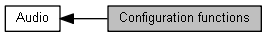
\includegraphics[width=274pt]{d0/df3/group___audio___init}
\end{center}
\end{figure}
\subsection*{Functions}
\begin{DoxyCompactItemize}
\item 
void \hyperlink{group___audio___init_gafff6cd7f4332d078ce0114143cd30998}{audio\+\_\+disable} (void)
\begin{DoxyCompactList}\small\item\em Disable the D\+MA. \end{DoxyCompactList}\item 
void \hyperlink{group___audio___init_gabcda20e7d4baa315d151230fcc81ec1d}{audio\+\_\+init} (uint16\+\_\+t $\ast$D\+A\+C\+Buffer, uint16\+\_\+t Size)
\begin{DoxyCompactList}\small\item\em Perform audio initialization. \end{DoxyCompactList}\end{DoxyCompactItemize}


\subsection{Detailed Description}
Audio configuration functions. 



\subsection{Function Documentation}
\index{Configuration functions@{Configuration functions}!audio\+\_\+disable@{audio\+\_\+disable}}
\index{audio\+\_\+disable@{audio\+\_\+disable}!Configuration functions@{Configuration functions}}
\subsubsection[{\texorpdfstring{audio\+\_\+disable(void)}{audio_disable(void)}}]{\setlength{\rightskip}{0pt plus 5cm}void audio\+\_\+disable (
\begin{DoxyParamCaption}
\item[{void}]{}
\end{DoxyParamCaption}
)}\hypertarget{group___audio___init_gafff6cd7f4332d078ce0114143cd30998}{}\label{group___audio___init_gafff6cd7f4332d078ce0114143cd30998}


Disable the D\+MA. 


\begin{DoxyParams}{Parameters}
{\em None} & \\
\hline
\end{DoxyParams}

\begin{DoxyRetVals}{Return values}
{\em None} & \\
\hline
\end{DoxyRetVals}


Definition at line 48 of file N\+P\+C\+\_\+audio.\+c.



Here is the caller graph for this function\+:\nopagebreak
\begin{figure}[H]
\begin{center}
\leavevmode
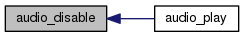
\includegraphics[width=255pt]{d0/df3/group___audio___init_gafff6cd7f4332d078ce0114143cd30998_icgraph}
\end{center}
\end{figure}


\index{Configuration functions@{Configuration functions}!audio\+\_\+init@{audio\+\_\+init}}
\index{audio\+\_\+init@{audio\+\_\+init}!Configuration functions@{Configuration functions}}
\subsubsection[{\texorpdfstring{audio\+\_\+init(uint16\+\_\+t $\ast$\+D\+A\+C\+Buffer, uint16\+\_\+t Size)}{audio_init(uint16_t *DACBuffer, uint16_t Size)}}]{\setlength{\rightskip}{0pt plus 5cm}void audio\+\_\+init (
\begin{DoxyParamCaption}
\item[{uint16\+\_\+t $\ast$}]{D\+A\+C\+Buffer, }
\item[{uint16\+\_\+t}]{Size}
\end{DoxyParamCaption}
)}\hypertarget{group___audio___init_gabcda20e7d4baa315d151230fcc81ec1d}{}\label{group___audio___init_gabcda20e7d4baa315d151230fcc81ec1d}


Perform audio initialization. 


\begin{DoxyParams}{Parameters}
{\em D\+A\+C\+Buffer} & Array to be pushed to the D\+MA \\
\hline
{\em Mode} & D\+MA Mode (default\+:D\+M\+A\+\_\+\+Mode\+\_\+\+Normal) \\
\hline
{\em Size} & sample size (default\+:S\+A\+M\+P\+L\+E\+\_\+\+S\+I\+ZE) \\
\hline
\end{DoxyParams}

\begin{DoxyRetVals}{Return values}
{\em None} & \\
\hline
\end{DoxyRetVals}


Definition at line 61 of file N\+P\+C\+\_\+audio.\+c.



Here is the caller graph for this function\+:\nopagebreak
\begin{figure}[H]
\begin{center}
\leavevmode
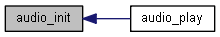
\includegraphics[width=237pt]{d0/df3/group___audio___init_gabcda20e7d4baa315d151230fcc81ec1d_icgraph}
\end{center}
\end{figure}



\hypertarget{group___audio___play}{}\section{Play audio functions}
\label{group___audio___play}\index{Play audio functions@{Play audio functions}}


Audio functions.  


Collaboration diagram for Play audio functions\+:\nopagebreak
\begin{figure}[H]
\begin{center}
\leavevmode
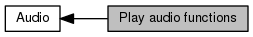
\includegraphics[width=262pt]{de/d72/group___audio___play}
\end{center}
\end{figure}
\subsection*{Functions}
\begin{DoxyCompactItemize}
\item 
void \hyperlink{group___audio___play_gaf73a37418a80bbb39f75abe8b60b0afb}{audio\+\_\+play} (uint16\+\_\+t $\ast$D\+A\+C\+Buffer, uint16\+\_\+t Size)
\begin{DoxyCompactList}\small\item\em Play a sample. \end{DoxyCompactList}\end{DoxyCompactItemize}


\subsection{Detailed Description}
Audio functions. 



\subsection{Function Documentation}
\index{Play audio functions@{Play audio functions}!audio\+\_\+play@{audio\+\_\+play}}
\index{audio\+\_\+play@{audio\+\_\+play}!Play audio functions@{Play audio functions}}
\subsubsection[{\texorpdfstring{audio\+\_\+play(uint16\+\_\+t $\ast$\+D\+A\+C\+Buffer, uint16\+\_\+t Size)}{audio_play(uint16_t *DACBuffer, uint16_t Size)}}]{\setlength{\rightskip}{0pt plus 5cm}void audio\+\_\+play (
\begin{DoxyParamCaption}
\item[{uint16\+\_\+t $\ast$}]{D\+A\+C\+Buffer, }
\item[{uint16\+\_\+t}]{Size}
\end{DoxyParamCaption}
)}\hypertarget{group___audio___play_gaf73a37418a80bbb39f75abe8b60b0afb}{}\label{group___audio___play_gaf73a37418a80bbb39f75abe8b60b0afb}


Play a sample. 


\begin{DoxyParams}{Parameters}
{\em D\+A\+C\+Buffer} & Array to be pushed to the D\+MA \\
\hline
{\em Size} & sample size (default\+:S\+A\+M\+P\+L\+E\+\_\+\+S\+I\+ZE) \\
\hline
\end{DoxyParams}
\begin{DoxyReturn}{Returns}
None 
\end{DoxyReturn}


Definition at line 136 of file N\+P\+C\+\_\+audio.\+c.



Here is the call graph for this function\+:\nopagebreak
\begin{figure}[H]
\begin{center}
\leavevmode
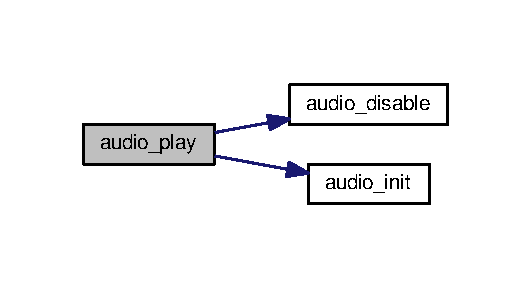
\includegraphics[width=255pt]{de/d72/group___audio___play_gaf73a37418a80bbb39f75abe8b60b0afb_cgraph}
\end{center}
\end{figure}



\hypertarget{group___bluetooth}{}\section{Bluetooth}
\label{group___bluetooth}\index{Bluetooth@{Bluetooth}}


Bluetooth driver modules.  


\subsection*{Modules}
\begin{DoxyCompactItemize}
\item 
\hyperlink{group___bluetooth___init}{Initialization and transmission handler functions}
\begin{DoxyCompactList}\small\item\em Bluetooth initialization functions. \end{DoxyCompactList}\item 
\hyperlink{group___bluetooth___trans}{Transmission functions}
\begin{DoxyCompactList}\small\item\em Bluetooth transmission functions. \end{DoxyCompactList}\end{DoxyCompactItemize}
\subsection*{Functions}
\begin{DoxyCompactItemize}
\item 
void \hyperlink{group___bluetooth_gaaa60810e0857e9e1e5b2cba80b8db3ff}{bluetooth\+\_\+init} (void)
\begin{DoxyCompactList}\small\item\em Initialize the bluetooth and set baudrate to 9600. \end{DoxyCompactList}\item 
void \hyperlink{group___bluetooth_ga7139cd4baabbbcbab0c1fe6d7d4ae1cc}{U\+S\+A\+R\+T1\+\_\+\+I\+R\+Q\+Handler} (void)
\begin{DoxyCompactList}\small\item\em U\+S\+A\+R\+T1 Interrupt Handler. \end{DoxyCompactList}\item 
void \hyperlink{group___bluetooth_ga31d829d5658369ee2c90b9c3cdbedfe1}{bluetooth\+\_\+send} (uint8\+\_\+t $\ast$data)
\begin{DoxyCompactList}\small\item\em send string to the hc-\/06 \end{DoxyCompactList}\item 
uint8\+\_\+t \hyperlink{group___bluetooth_gab7ad1e1b94cf1cedc8a8e5151b0e25cb}{bluetooth\+\_\+receive} (void)
\begin{DoxyCompactList}\small\item\em receive a byte from hc-\/06 \end{DoxyCompactList}\end{DoxyCompactItemize}


\subsection{Detailed Description}
Bluetooth driver modules. 



\subsection{Function Documentation}
\mbox{\Hypertarget{group___bluetooth_gaaa60810e0857e9e1e5b2cba80b8db3ff}\label{group___bluetooth_gaaa60810e0857e9e1e5b2cba80b8db3ff}} 
\index{Bluetooth@{Bluetooth}!bluetooth\+\_\+init@{bluetooth\+\_\+init}}
\index{bluetooth\+\_\+init@{bluetooth\+\_\+init}!Bluetooth@{Bluetooth}}
\subsubsection{\texorpdfstring{bluetooth\+\_\+init()}{bluetooth\_init()}}
{\footnotesize\ttfamily void bluetooth\+\_\+init (\begin{DoxyParamCaption}\item[{void}]{ }\end{DoxyParamCaption})}



Initialize the bluetooth and set baudrate to 9600. 


\begin{DoxyParams}{Parameters}
{\em None} & \\
\hline
\end{DoxyParams}

\begin{DoxyRetVals}{Return values}
{\em None} & \\
\hline
\end{DoxyRetVals}
\mbox{\Hypertarget{group___bluetooth_gab7ad1e1b94cf1cedc8a8e5151b0e25cb}\label{group___bluetooth_gab7ad1e1b94cf1cedc8a8e5151b0e25cb}} 
\index{Bluetooth@{Bluetooth}!bluetooth\+\_\+receive@{bluetooth\+\_\+receive}}
\index{bluetooth\+\_\+receive@{bluetooth\+\_\+receive}!Bluetooth@{Bluetooth}}
\subsubsection{\texorpdfstring{bluetooth\+\_\+receive()}{bluetooth\_receive()}}
{\footnotesize\ttfamily uint8\+\_\+t bluetooth\+\_\+receive (\begin{DoxyParamCaption}\item[{void}]{ }\end{DoxyParamCaption})}



receive a byte from hc-\/06 


\begin{DoxyParams}{Parameters}
{\em None} & \\
\hline
\end{DoxyParams}

\begin{DoxyRetVals}{Return values}
{\em An} & uint8\+\_\+t byte of data \\
\hline
\end{DoxyRetVals}
\mbox{\Hypertarget{group___bluetooth_ga31d829d5658369ee2c90b9c3cdbedfe1}\label{group___bluetooth_ga31d829d5658369ee2c90b9c3cdbedfe1}} 
\index{Bluetooth@{Bluetooth}!bluetooth\+\_\+send@{bluetooth\+\_\+send}}
\index{bluetooth\+\_\+send@{bluetooth\+\_\+send}!Bluetooth@{Bluetooth}}
\subsubsection{\texorpdfstring{bluetooth\+\_\+send()}{bluetooth\_send()}}
{\footnotesize\ttfamily void bluetooth\+\_\+send (\begin{DoxyParamCaption}\item[{uint8\+\_\+t $\ast$}]{data }\end{DoxyParamCaption})}



send string to the hc-\/06 


\begin{DoxyParams}{Parameters}
{\em data} & string to be sent \\
\hline
\end{DoxyParams}

\begin{DoxyRetVals}{Return values}
{\em None} & \\
\hline
\end{DoxyRetVals}
\mbox{\Hypertarget{group___bluetooth_ga7139cd4baabbbcbab0c1fe6d7d4ae1cc}\label{group___bluetooth_ga7139cd4baabbbcbab0c1fe6d7d4ae1cc}} 
\index{Bluetooth@{Bluetooth}!U\+S\+A\+R\+T1\+\_\+\+I\+R\+Q\+Handler@{U\+S\+A\+R\+T1\+\_\+\+I\+R\+Q\+Handler}}
\index{U\+S\+A\+R\+T1\+\_\+\+I\+R\+Q\+Handler@{U\+S\+A\+R\+T1\+\_\+\+I\+R\+Q\+Handler}!Bluetooth@{Bluetooth}}
\subsubsection{\texorpdfstring{U\+S\+A\+R\+T1\+\_\+\+I\+R\+Q\+Handler()}{USART1\_IRQHandler()}}
{\footnotesize\ttfamily void U\+S\+A\+R\+T1\+\_\+\+I\+R\+Q\+Handler (\begin{DoxyParamCaption}\item[{void}]{ }\end{DoxyParamCaption})}



U\+S\+A\+R\+T1 Interrupt Handler. 


\begin{DoxyParams}{Parameters}
{\em None} & \\
\hline
\end{DoxyParams}

\begin{DoxyRetVals}{Return values}
{\em none} & \\
\hline
\end{DoxyRetVals}

\hypertarget{group___bluetooth___init}{}\section{Initialization and transmission handler functions}
\label{group___bluetooth___init}\index{Initialization and transmission handler functions@{Initialization and transmission handler functions}}


Bluetooth initialization functions.  


\subsection*{Functions}
\begin{DoxyCompactItemize}
\item 
void \hyperlink{group___bluetooth___init_gaaa60810e0857e9e1e5b2cba80b8db3ff}{bluetooth\+\_\+init} (void)
\begin{DoxyCompactList}\small\item\em Initialize the bluetooth and set baudrate to 9600. \end{DoxyCompactList}\item 
void \hyperlink{group___bluetooth___init_ga7139cd4baabbbcbab0c1fe6d7d4ae1cc}{U\+S\+A\+R\+T1\+\_\+\+I\+R\+Q\+Handler} (void)
\begin{DoxyCompactList}\small\item\em U\+S\+A\+R\+T1 Interrupt Handler. \end{DoxyCompactList}\end{DoxyCompactItemize}


\subsection{Detailed Description}
Bluetooth initialization functions. 



\subsection{Function Documentation}
\mbox{\Hypertarget{group___bluetooth___init_gaaa60810e0857e9e1e5b2cba80b8db3ff}\label{group___bluetooth___init_gaaa60810e0857e9e1e5b2cba80b8db3ff}} 
\index{Initialization and transmission handler functions@{Initialization and transmission handler functions}!bluetooth\+\_\+init@{bluetooth\+\_\+init}}
\index{bluetooth\+\_\+init@{bluetooth\+\_\+init}!Initialization and transmission handler functions@{Initialization and transmission handler functions}}
\subsubsection{\texorpdfstring{bluetooth\+\_\+init()}{bluetooth\_init()}}
{\footnotesize\ttfamily void bluetooth\+\_\+init (\begin{DoxyParamCaption}\item[{void}]{ }\end{DoxyParamCaption})}



Initialize the bluetooth and set baudrate to 9600. 


\begin{DoxyParams}{Parameters}
{\em None} & \\
\hline
\end{DoxyParams}

\begin{DoxyRetVals}{Return values}
{\em None} & \\
\hline
\end{DoxyRetVals}
\mbox{\Hypertarget{group___bluetooth___init_ga7139cd4baabbbcbab0c1fe6d7d4ae1cc}\label{group___bluetooth___init_ga7139cd4baabbbcbab0c1fe6d7d4ae1cc}} 
\index{Initialization and transmission handler functions@{Initialization and transmission handler functions}!U\+S\+A\+R\+T1\+\_\+\+I\+R\+Q\+Handler@{U\+S\+A\+R\+T1\+\_\+\+I\+R\+Q\+Handler}}
\index{U\+S\+A\+R\+T1\+\_\+\+I\+R\+Q\+Handler@{U\+S\+A\+R\+T1\+\_\+\+I\+R\+Q\+Handler}!Initialization and transmission handler functions@{Initialization and transmission handler functions}}
\subsubsection{\texorpdfstring{U\+S\+A\+R\+T1\+\_\+\+I\+R\+Q\+Handler()}{USART1\_IRQHandler()}}
{\footnotesize\ttfamily void U\+S\+A\+R\+T1\+\_\+\+I\+R\+Q\+Handler (\begin{DoxyParamCaption}\item[{void}]{ }\end{DoxyParamCaption})}



U\+S\+A\+R\+T1 Interrupt Handler. 


\begin{DoxyParams}{Parameters}
{\em None} & \\
\hline
\end{DoxyParams}

\begin{DoxyRetVals}{Return values}
{\em none} & \\
\hline
\end{DoxyRetVals}

\hypertarget{group___bluetooth___trans}{}\section{Transmission functions}
\label{group___bluetooth___trans}\index{Transmission functions@{Transmission functions}}


Bluetooth transmission functions.  


Collaboration diagram for Transmission functions\+:
% FIG 0
\subsection*{Functions}
\begin{DoxyCompactItemize}
\item 
void \hyperlink{group___bluetooth___trans_ga31d829d5658369ee2c90b9c3cdbedfe1}{bluetooth\+\_\+send} (uint8\+\_\+t $\ast$data)
\begin{DoxyCompactList}\small\item\em send string to the hc-\/06 \end{DoxyCompactList}\item 
uint8\+\_\+t \hyperlink{group___bluetooth___trans_gab7ad1e1b94cf1cedc8a8e5151b0e25cb}{bluetooth\+\_\+receive} (void)
\begin{DoxyCompactList}\small\item\em receive a byte from hc-\/06 \end{DoxyCompactList}\end{DoxyCompactItemize}


\subsection{Detailed Description}
Bluetooth transmission functions. 



\subsection{Function Documentation}
\mbox{\Hypertarget{group___bluetooth___trans_gab7ad1e1b94cf1cedc8a8e5151b0e25cb}\label{group___bluetooth___trans_gab7ad1e1b94cf1cedc8a8e5151b0e25cb}} 
\index{Transmission functions@{Transmission functions}!bluetooth\+\_\+receive@{bluetooth\+\_\+receive}}
\index{bluetooth\+\_\+receive@{bluetooth\+\_\+receive}!Transmission functions@{Transmission functions}}
\subsubsection{\texorpdfstring{bluetooth\+\_\+receive()}{bluetooth\_receive()}}
{\footnotesize\ttfamily uint8\+\_\+t bluetooth\+\_\+receive (\begin{DoxyParamCaption}\item[{void}]{ }\end{DoxyParamCaption})}



receive a byte from hc-\/06 


\begin{DoxyParams}{Parameters}
{\em None} & \\
\hline
\end{DoxyParams}

\begin{DoxyRetVals}{Return values}
{\em An} & uint8\+\_\+t byte of data \\
\hline
\end{DoxyRetVals}
\mbox{\Hypertarget{group___bluetooth___trans_ga31d829d5658369ee2c90b9c3cdbedfe1}\label{group___bluetooth___trans_ga31d829d5658369ee2c90b9c3cdbedfe1}} 
\index{Transmission functions@{Transmission functions}!bluetooth\+\_\+send@{bluetooth\+\_\+send}}
\index{bluetooth\+\_\+send@{bluetooth\+\_\+send}!Transmission functions@{Transmission functions}}
\subsubsection{\texorpdfstring{bluetooth\+\_\+send()}{bluetooth\_send()}}
{\footnotesize\ttfamily void bluetooth\+\_\+send (\begin{DoxyParamCaption}\item[{uint8\+\_\+t $\ast$}]{data }\end{DoxyParamCaption})}



send string to the hc-\/06 


\begin{DoxyParams}{Parameters}
{\em data} & string to be sent \\
\hline
\end{DoxyParams}

\begin{DoxyRetVals}{Return values}
{\em None} & \\
\hline
\end{DoxyRetVals}

\hypertarget{group___clock}{}\section{Clock}
\label{group___clock}\index{Clock@{Clock}}


Clock driver modules.  


Collaboration diagram for Clock\+:
% FIG 0
\subsection*{Modules}
\begin{DoxyCompactItemize}
\item 
\hyperlink{group___r_t_c___p_r_e_d_i_v___definitions}{R\+T\+C\+\_\+\+P\+R\+E\+D\+I\+V\+\_\+\+Definitions}
\begin{DoxyCompactList}\small\item\em definition of prescaler for Asynchronous and Synchronous \end{DoxyCompactList}\item 
\hyperlink{group___c_l_o_c_k___choice}{C\+L\+O\+C\+K\+\_\+\+Choice}
\begin{DoxyCompactList}\small\item\em Clock A or B. \end{DoxyCompactList}\item 
\hyperlink{group___c_l_o_c_k___format}{C\+L\+O\+C\+K\+\_\+\+Format}
\begin{DoxyCompactList}\small\item\em AM or PM. \end{DoxyCompactList}\item 
\hyperlink{group___c_l_o_c_k___value}{C\+L\+O\+C\+K\+\_\+\+Value}
\begin{DoxyCompactList}\small\item\em Access time or date parameters. \end{DoxyCompactList}\item 
\hyperlink{group___r_e_p_e_a_t___definitions}{R\+E\+P\+E\+A\+T\+\_\+\+Definitions}
\begin{DoxyCompactList}\small\item\em Alarm repeat options. \end{DoxyCompactList}\item 
\hyperlink{group___clock___init}{Initialisation functions}
\begin{DoxyCompactList}\small\item\em Clock initialisation functions. \end{DoxyCompactList}\item 
\hyperlink{group___clock___time___date}{Time and Date Configuration functions}
\begin{DoxyCompactList}\small\item\em Clock time and date configuration functions. \end{DoxyCompactList}\item 
\hyperlink{group___clock___alarms}{Alarms configuration functions}
\begin{DoxyCompactList}\small\item\em Clock alarm configuration functions. \end{DoxyCompactList}\end{DoxyCompactItemize}
\subsection*{Functions}
\begin{DoxyCompactItemize}
\item 
void \hyperlink{group___clock_ga78ab77b57cf2e00089f0a3a22508524c}{clock\+\_\+init} (void)
\begin{DoxyCompactList}\small\item\em Initialise the clock to 1\+Hz and setup peripherals for Alarm. \end{DoxyCompactList}\item 
Error\+Status \hyperlink{group___clock_gaf16498fa2702bfda6b89a3335ccc7ca6}{clock\+\_\+set\+Date} (uint8\+\_\+t week\+Day, uint8\+\_\+t month, uint8\+\_\+t date, uint8\+\_\+t year)
\begin{DoxyCompactList}\small\item\em Set the clock\textquotesingle{}s date. \end{DoxyCompactList}\item 
Error\+Status \hyperlink{group___clock_ga11404197d58ddf6b46230bcde4282ef2}{clock\+\_\+set\+Time} (uint8\+\_\+t am\+\_\+pm, uint8\+\_\+t hours, uint8\+\_\+t minutes, uint8\+\_\+t second)
\begin{DoxyCompactList}\small\item\em Set the clock\textquotesingle{}s time. \end{DoxyCompactList}\item 
uint32\+\_\+t \hyperlink{group___clock_gabb4d72928cb3d131d40067fb141003aa}{clock\+\_\+get\+Date} (void)
\begin{DoxyCompactList}\small\item\em Get the date encoded in a 32b format. \end{DoxyCompactList}\item 
uint32\+\_\+t \hyperlink{group___clock_ga03ae6948083c259f6edc0b146f40dc62}{clock\+\_\+get\+Time} (void)
\begin{DoxyCompactList}\small\item\em Get the time encoded in a 32b format. \end{DoxyCompactList}\item 
R\+T\+C\+\_\+\+Alarm\+Type\+Def \hyperlink{group___clock_ga5e1614dbb1a210106dbade3f133db27e}{clock\+\_\+create\+Alarm} (uint8\+\_\+t am\+\_\+pm, uint8\+\_\+t hours, uint8\+\_\+t minutes, uint8\+\_\+t seconds, uint32\+\_\+t date\+Week\+Day\+Sel, uint8\+\_\+t date\+Week\+Day, uint32\+\_\+t repeat)
\begin{DoxyCompactList}\small\item\em Create an Alarm Structure given all the parameters. \end{DoxyCompactList}\item 
void \hyperlink{group___clock_gab56f512746d4f2638232db28bb7dac2b}{clock\+\_\+setA} (R\+T\+C\+\_\+\+Alarm\+Type\+Def $\ast$Alarm)
\begin{DoxyCompactList}\small\item\em Set an alarm to R\+T\+C\+\_\+\+Alarm\+\_\+A, given a Alarm structure R\+T\+C\+\_\+\+Alarm\+Type\+Def. \end{DoxyCompactList}\item 
void \hyperlink{group___clock_gaea1a099c4ad6de8b99517ac6453e3569}{clock\+\_\+set\+Alarm} (uint8\+\_\+t am\+\_\+pm, uint8\+\_\+t hours, uint8\+\_\+t minutes, uint8\+\_\+t seconds, uint32\+\_\+t date\+Week\+Day\+Sel, uint8\+\_\+t date\+Week\+Day, uint32\+\_\+t repeat)
\begin{DoxyCompactList}\small\item\em Set an alarm to R\+T\+C\+\_\+\+Alarm\+\_\+A, given all the alarm parameters. \end{DoxyCompactList}\item 
void \hyperlink{group___clock_ga4da4fb52ec579671d337938e78f9a207}{R\+T\+C\+\_\+\+Alarm\+\_\+\+I\+R\+Q\+Handler} (void)
\begin{DoxyCompactList}\small\item\em Alarm Handler. \end{DoxyCompactList}\end{DoxyCompactItemize}
\subsection*{Variables}
\begin{DoxyCompactItemize}
\item 
\mbox{\Hypertarget{group___clock_gab350523f036d8469fd207d7144f7e385}\label{group___clock_gab350523f036d8469fd207d7144f7e385}} 
R\+T\+C\+\_\+\+Time\+Type\+Def {\bfseries R\+T\+C\+\_\+\+Time\+Struct}
\item 
\mbox{\Hypertarget{group___clock_gabd73cfb4bb5c20ec4524dd5fe244842b}\label{group___clock_gabd73cfb4bb5c20ec4524dd5fe244842b}} 
R\+T\+C\+\_\+\+Init\+Type\+Def {\bfseries R\+T\+C\+\_\+\+Init\+Struct}
\item 
\mbox{\Hypertarget{group___clock_gaa57dd593e8f26c6f126fd0f694a1facc}\label{group___clock_gaa57dd593e8f26c6f126fd0f694a1facc}} 
R\+T\+C\+\_\+\+Date\+Type\+Def {\bfseries R\+T\+C\+\_\+\+Date\+Strcut}
\item 
\mbox{\Hypertarget{group___clock_ga64d4fe2aa4668079f349f9eb97a48e35}\label{group___clock_ga64d4fe2aa4668079f349f9eb97a48e35}} 
R\+T\+C\+\_\+\+Alarm\+Type\+Def {\bfseries R\+T\+C\+\_\+\+Alarm\+Struct}
\item 
\mbox{\Hypertarget{group___clock_gaf0f09eb6c46f0a7cc5f7736c709a8c77}\label{group___clock_gaf0f09eb6c46f0a7cc5f7736c709a8c77}} 
E\+X\+T\+I\+\_\+\+Init\+Type\+Def {\bfseries E\+X\+T\+I\+\_\+\+Init\+Struct}
\end{DoxyCompactItemize}


\subsection{Detailed Description}
Clock driver modules. 



\subsection{Function Documentation}
\mbox{\Hypertarget{group___clock_ga5e1614dbb1a210106dbade3f133db27e}\label{group___clock_ga5e1614dbb1a210106dbade3f133db27e}} 
\index{Clock@{Clock}!clock\+\_\+create\+Alarm@{clock\+\_\+create\+Alarm}}
\index{clock\+\_\+create\+Alarm@{clock\+\_\+create\+Alarm}!Clock@{Clock}}
\subsubsection{\texorpdfstring{clock\+\_\+create\+Alarm()}{clock\_createAlarm()}}
{\footnotesize\ttfamily R\+T\+C\+\_\+\+Alarm\+Type\+Def clock\+\_\+create\+Alarm (\begin{DoxyParamCaption}\item[{uint8\+\_\+t}]{am\+\_\+pm,  }\item[{uint8\+\_\+t}]{hours,  }\item[{uint8\+\_\+t}]{minutes,  }\item[{uint8\+\_\+t}]{seconds,  }\item[{uint32\+\_\+t}]{date\+Week\+Day\+Sel,  }\item[{uint8\+\_\+t}]{date\+Week\+Day,  }\item[{uint32\+\_\+t}]{repeat }\end{DoxyParamCaption})}



Create an Alarm Structure given all the parameters. 


\begin{DoxyParams}{Parameters}
{\em am\+\_\+pm} & AM PM format (C\+L\+O\+C\+K\+\_\+\+AM) \\
\hline
{\em hours} & Alarm hours \\
\hline
{\em minutes} & Alarm minutes \\
\hline
{\em seconds} & Alarm seconds \\
\hline
{\em date\+Week\+Day\+Sel} & Date of Week\+Day selection R\+T\+C\+\_\+\+Alarm\+Date\+Week\+Day\+\_\+\+Definitions \\
\hline
{\em date\+Week\+Day} & Specify Alarm Date/\+Weekday if Date then value range from 1-\/31, else R\+T\+C\+\_\+\+Week\+Day\+\_\+\+Definitions \\
\hline
{\em repeat} & Specify the repetition of the Alarm \\
\hline
\end{DoxyParams}

\begin{DoxyRetVals}{Return values}
{\em An} & R\+T\+C\+\_\+\+Alarm\+Type\+Def containing all the parameters above \\
\hline
\end{DoxyRetVals}
\mbox{\Hypertarget{group___clock_gabb4d72928cb3d131d40067fb141003aa}\label{group___clock_gabb4d72928cb3d131d40067fb141003aa}} 
\index{Clock@{Clock}!clock\+\_\+get\+Date@{clock\+\_\+get\+Date}}
\index{clock\+\_\+get\+Date@{clock\+\_\+get\+Date}!Clock@{Clock}}
\subsubsection{\texorpdfstring{clock\+\_\+get\+Date()}{clock\_getDate()}}
{\footnotesize\ttfamily uint32\+\_\+t clock\+\_\+get\+Date (\begin{DoxyParamCaption}\item[{void}]{ }\end{DoxyParamCaption})}



Get the date encoded in a 32b format. 


\begin{DoxyParams}{Parameters}
{\em None} & \\
\hline
\end{DoxyParams}

\begin{DoxyRetVals}{Return values}
{\em An} & uint32\+\_\+t containing the week\+Day as its M\+B3, date \+: M\+B2, month \+: M\+B1, year \+: M\+B0 \\
\hline
\end{DoxyRetVals}
\mbox{\Hypertarget{group___clock_ga03ae6948083c259f6edc0b146f40dc62}\label{group___clock_ga03ae6948083c259f6edc0b146f40dc62}} 
\index{Clock@{Clock}!clock\+\_\+get\+Time@{clock\+\_\+get\+Time}}
\index{clock\+\_\+get\+Time@{clock\+\_\+get\+Time}!Clock@{Clock}}
\subsubsection{\texorpdfstring{clock\+\_\+get\+Time()}{clock\_getTime()}}
{\footnotesize\ttfamily uint32\+\_\+t clock\+\_\+get\+Time (\begin{DoxyParamCaption}\item[{void}]{ }\end{DoxyParamCaption})}



Get the time encoded in a 32b format. 


\begin{DoxyParams}{Parameters}
{\em None} & \\
\hline
\end{DoxyParams}

\begin{DoxyRetVals}{Return values}
{\em An} & uint32\+\_\+t containing the hour as its M\+B3, minutes \+: M\+B2, Seconds \+: M\+B1, format \+: M\+B0 \\
\hline
\end{DoxyRetVals}
\mbox{\Hypertarget{group___clock_ga78ab77b57cf2e00089f0a3a22508524c}\label{group___clock_ga78ab77b57cf2e00089f0a3a22508524c}} 
\index{Clock@{Clock}!clock\+\_\+init@{clock\+\_\+init}}
\index{clock\+\_\+init@{clock\+\_\+init}!Clock@{Clock}}
\subsubsection{\texorpdfstring{clock\+\_\+init()}{clock\_init()}}
{\footnotesize\ttfamily void clock\+\_\+init (\begin{DoxyParamCaption}\item[{void}]{ }\end{DoxyParamCaption})}



Initialise the clock to 1\+Hz and setup peripherals for Alarm. 


\begin{DoxyParams}{Parameters}
{\em None} & \\
\hline
\end{DoxyParams}

\begin{DoxyRetVals}{Return values}
{\em None} & \\
\hline
\end{DoxyRetVals}
\mbox{\Hypertarget{group___clock_gab56f512746d4f2638232db28bb7dac2b}\label{group___clock_gab56f512746d4f2638232db28bb7dac2b}} 
\index{Clock@{Clock}!clock\+\_\+setA@{clock\+\_\+setA}}
\index{clock\+\_\+setA@{clock\+\_\+setA}!Clock@{Clock}}
\subsubsection{\texorpdfstring{clock\+\_\+set\+A()}{clock\_setA()}}
{\footnotesize\ttfamily void clock\+\_\+setA (\begin{DoxyParamCaption}\item[{R\+T\+C\+\_\+\+Alarm\+Type\+Def $\ast$}]{Alarm }\end{DoxyParamCaption})}



Set an alarm to R\+T\+C\+\_\+\+Alarm\+\_\+A, given a Alarm structure R\+T\+C\+\_\+\+Alarm\+Type\+Def. 


\begin{DoxyParams}{Parameters}
{\em Alarm} & A pointer to the R\+T\+C\+\_\+\+Alarm\+Type\+Def \\
\hline
\end{DoxyParams}

\begin{DoxyRetVals}{Return values}
{\em None} & \\
\hline
\end{DoxyRetVals}
\mbox{\Hypertarget{group___clock_gaea1a099c4ad6de8b99517ac6453e3569}\label{group___clock_gaea1a099c4ad6de8b99517ac6453e3569}} 
\index{Clock@{Clock}!clock\+\_\+set\+Alarm@{clock\+\_\+set\+Alarm}}
\index{clock\+\_\+set\+Alarm@{clock\+\_\+set\+Alarm}!Clock@{Clock}}
\subsubsection{\texorpdfstring{clock\+\_\+set\+Alarm()}{clock\_setAlarm()}}
{\footnotesize\ttfamily void clock\+\_\+set\+Alarm (\begin{DoxyParamCaption}\item[{uint8\+\_\+t}]{am\+\_\+pm,  }\item[{uint8\+\_\+t}]{hours,  }\item[{uint8\+\_\+t}]{minutes,  }\item[{uint8\+\_\+t}]{seconds,  }\item[{uint32\+\_\+t}]{date\+Week\+Day\+Sel,  }\item[{uint8\+\_\+t}]{date\+Week\+Day,  }\item[{uint32\+\_\+t}]{repeat }\end{DoxyParamCaption})}



Set an alarm to R\+T\+C\+\_\+\+Alarm\+\_\+A, given all the alarm parameters. 


\begin{DoxyParams}{Parameters}
{\em am\+\_\+pm} & AM PM format (C\+L\+O\+C\+K\+\_\+\+AM) \\
\hline
{\em hours} & Alarm hours \\
\hline
{\em minutes} & Alarm minutes \\
\hline
{\em seconds} & Alarm seconds \\
\hline
{\em date\+Week\+Day\+Sel} & Date of Week\+Day selection R\+T\+C\+\_\+\+Alarm\+Date\+Week\+Day\+\_\+\+Definitions \\
\hline
{\em date\+Week\+Day} & Specify Alarm Date/\+Weekday if Date then value range from 1-\/31, else R\+T\+C\+\_\+\+Week\+Day\+\_\+\+Definitions \\
\hline
{\em repeat} & Specify the repetition of the Alarm \\
\hline
\end{DoxyParams}

\begin{DoxyRetVals}{Return values}
{\em None} & \\
\hline
\end{DoxyRetVals}
\mbox{\Hypertarget{group___clock_gaf16498fa2702bfda6b89a3335ccc7ca6}\label{group___clock_gaf16498fa2702bfda6b89a3335ccc7ca6}} 
\index{Clock@{Clock}!clock\+\_\+set\+Date@{clock\+\_\+set\+Date}}
\index{clock\+\_\+set\+Date@{clock\+\_\+set\+Date}!Clock@{Clock}}
\subsubsection{\texorpdfstring{clock\+\_\+set\+Date()}{clock\_setDate()}}
{\footnotesize\ttfamily Error\+Status clock\+\_\+set\+Date (\begin{DoxyParamCaption}\item[{uint8\+\_\+t}]{week\+Day,  }\item[{uint8\+\_\+t}]{month,  }\item[{uint8\+\_\+t}]{date,  }\item[{uint8\+\_\+t}]{year }\end{DoxyParamCaption})}



Set the clock\textquotesingle{}s date. 


\begin{DoxyParams}{Parameters}
{\em None} & \\
\hline
\end{DoxyParams}

\begin{DoxyRetVals}{Return values}
{\em Error\+Status} & representing the outcome of the operation
\begin{DoxyItemize}
\item S\+U\+C\+C\+E\+SS\+: R\+TC Shift registers are configured
\item E\+R\+R\+OR\+: R\+TC Shift registers are not configured 
\end{DoxyItemize}\\
\hline
\end{DoxyRetVals}
\mbox{\Hypertarget{group___clock_ga11404197d58ddf6b46230bcde4282ef2}\label{group___clock_ga11404197d58ddf6b46230bcde4282ef2}} 
\index{Clock@{Clock}!clock\+\_\+set\+Time@{clock\+\_\+set\+Time}}
\index{clock\+\_\+set\+Time@{clock\+\_\+set\+Time}!Clock@{Clock}}
\subsubsection{\texorpdfstring{clock\+\_\+set\+Time()}{clock\_setTime()}}
{\footnotesize\ttfamily Error\+Status clock\+\_\+set\+Time (\begin{DoxyParamCaption}\item[{uint8\+\_\+t}]{am\+\_\+pm,  }\item[{uint8\+\_\+t}]{hours,  }\item[{uint8\+\_\+t}]{minutes,  }\item[{uint8\+\_\+t}]{second }\end{DoxyParamCaption})}



Set the clock\textquotesingle{}s time. 


\begin{DoxyParams}{Parameters}
{\em None} & \\
\hline
\end{DoxyParams}

\begin{DoxyRetVals}{Return values}
{\em Error\+Status} & representing the outcome of the operation
\begin{DoxyItemize}
\item S\+U\+C\+C\+E\+SS\+: R\+TC Shift registers are configured
\item E\+R\+R\+OR\+: R\+TC Shift registers are not configured 
\end{DoxyItemize}\\
\hline
\end{DoxyRetVals}
\mbox{\Hypertarget{group___clock_ga4da4fb52ec579671d337938e78f9a207}\label{group___clock_ga4da4fb52ec579671d337938e78f9a207}} 
\index{Clock@{Clock}!R\+T\+C\+\_\+\+Alarm\+\_\+\+I\+R\+Q\+Handler@{R\+T\+C\+\_\+\+Alarm\+\_\+\+I\+R\+Q\+Handler}}
\index{R\+T\+C\+\_\+\+Alarm\+\_\+\+I\+R\+Q\+Handler@{R\+T\+C\+\_\+\+Alarm\+\_\+\+I\+R\+Q\+Handler}!Clock@{Clock}}
\subsubsection{\texorpdfstring{R\+T\+C\+\_\+\+Alarm\+\_\+\+I\+R\+Q\+Handler()}{RTC\_Alarm\_IRQHandler()}}
{\footnotesize\ttfamily void R\+T\+C\+\_\+\+Alarm\+\_\+\+I\+R\+Q\+Handler (\begin{DoxyParamCaption}\item[{void}]{ }\end{DoxyParamCaption})}



Alarm Handler. 


\begin{DoxyParams}{Parameters}
{\em None} & \\
\hline
\end{DoxyParams}

\begin{DoxyRetVals}{Return values}
{\em None} & \\
\hline
\end{DoxyRetVals}

\hypertarget{group___clock___init}{}\section{Initialisation functions}
\label{group___clock___init}\index{Initialisation functions@{Initialisation functions}}


Clock initialisation functions.  


Collaboration diagram for Initialisation functions\+:\nopagebreak
\begin{figure}[H]
\begin{center}
\leavevmode
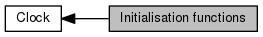
\includegraphics[width=269pt]{dd/d06/group___clock___init}
\end{center}
\end{figure}
\subsection*{Functions}
\begin{DoxyCompactItemize}
\item 
void \hyperlink{group___clock___init_ga78ab77b57cf2e00089f0a3a22508524c}{clock\+\_\+init} (void)
\begin{DoxyCompactList}\small\item\em Initialise the clock to 1\+Hz and setup peripherals for Alarm. \end{DoxyCompactList}\end{DoxyCompactItemize}


\subsection{Detailed Description}
Clock initialisation functions. 



\subsection{Function Documentation}
\index{Initialisation functions@{Initialisation functions}!clock\+\_\+init@{clock\+\_\+init}}
\index{clock\+\_\+init@{clock\+\_\+init}!Initialisation functions@{Initialisation functions}}
\subsubsection[{\texorpdfstring{clock\+\_\+init(void)}{clock_init(void)}}]{\setlength{\rightskip}{0pt plus 5cm}void clock\+\_\+init (
\begin{DoxyParamCaption}
\item[{void}]{}
\end{DoxyParamCaption}
)}\hypertarget{group___clock___init_ga78ab77b57cf2e00089f0a3a22508524c}{}\label{group___clock___init_ga78ab77b57cf2e00089f0a3a22508524c}


Initialise the clock to 1\+Hz and setup peripherals for Alarm. 


\begin{DoxyParams}{Parameters}
{\em None} & \\
\hline
\end{DoxyParams}

\begin{DoxyRetVals}{Return values}
{\em None} & \\
\hline
\end{DoxyRetVals}


Definition at line 74 of file N\+P\+C\+\_\+clock.\+c.



Here is the caller graph for this function\+:\nopagebreak
\begin{figure}[H]
\begin{center}
\leavevmode
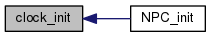
\includegraphics[width=230pt]{dd/d06/group___clock___init_ga78ab77b57cf2e00089f0a3a22508524c_icgraph}
\end{center}
\end{figure}



\hypertarget{group___clock___time___date}{}\section{Time and Date Configuration functions}
\label{group___clock___time___date}\index{Time and Date Configuration functions@{Time and Date Configuration functions}}


Clock time and date configuration functions.  


\subsection*{Functions}
\begin{DoxyCompactItemize}
\item 
Error\+Status \hyperlink{group___clock___time___date_gaf16498fa2702bfda6b89a3335ccc7ca6}{clock\+\_\+set\+Date} (uint8\+\_\+t week\+Day, uint8\+\_\+t month, uint8\+\_\+t date, uint8\+\_\+t year)
\begin{DoxyCompactList}\small\item\em Set the clock\textquotesingle{}s date. \end{DoxyCompactList}\item 
Error\+Status \hyperlink{group___clock___time___date_ga11404197d58ddf6b46230bcde4282ef2}{clock\+\_\+set\+Time} (uint8\+\_\+t am\+\_\+pm, uint8\+\_\+t hours, uint8\+\_\+t minutes, uint8\+\_\+t second)
\begin{DoxyCompactList}\small\item\em Set the clock\textquotesingle{}s time. \end{DoxyCompactList}\item 
uint32\+\_\+t \hyperlink{group___clock___time___date_gabb4d72928cb3d131d40067fb141003aa}{clock\+\_\+get\+Date} (void)
\begin{DoxyCompactList}\small\item\em Get the date encoded in a 32b format. \end{DoxyCompactList}\item 
uint32\+\_\+t \hyperlink{group___clock___time___date_ga03ae6948083c259f6edc0b146f40dc62}{clock\+\_\+get\+Time} (void)
\begin{DoxyCompactList}\small\item\em Get the time encoded in a 32b format. \end{DoxyCompactList}\end{DoxyCompactItemize}


\subsection{Detailed Description}
Clock time and date configuration functions. 



\subsection{Function Documentation}
\mbox{\Hypertarget{group___clock___time___date_gabb4d72928cb3d131d40067fb141003aa}\label{group___clock___time___date_gabb4d72928cb3d131d40067fb141003aa}} 
\index{Time and Date Configuration functions@{Time and Date Configuration functions}!clock\+\_\+get\+Date@{clock\+\_\+get\+Date}}
\index{clock\+\_\+get\+Date@{clock\+\_\+get\+Date}!Time and Date Configuration functions@{Time and Date Configuration functions}}
\subsubsection{\texorpdfstring{clock\+\_\+get\+Date()}{clock\_getDate()}}
{\footnotesize\ttfamily uint32\+\_\+t clock\+\_\+get\+Date (\begin{DoxyParamCaption}\item[{void}]{ }\end{DoxyParamCaption})}



Get the date encoded in a 32b format. 


\begin{DoxyParams}{Parameters}
{\em None} & \\
\hline
\end{DoxyParams}

\begin{DoxyRetVals}{Return values}
{\em An} & uint32\+\_\+t containing the week\+Day as its M\+B3, date \+: M\+B2, month \+: M\+B1, year \+: M\+B0 \\
\hline
\end{DoxyRetVals}
\mbox{\Hypertarget{group___clock___time___date_ga03ae6948083c259f6edc0b146f40dc62}\label{group___clock___time___date_ga03ae6948083c259f6edc0b146f40dc62}} 
\index{Time and Date Configuration functions@{Time and Date Configuration functions}!clock\+\_\+get\+Time@{clock\+\_\+get\+Time}}
\index{clock\+\_\+get\+Time@{clock\+\_\+get\+Time}!Time and Date Configuration functions@{Time and Date Configuration functions}}
\subsubsection{\texorpdfstring{clock\+\_\+get\+Time()}{clock\_getTime()}}
{\footnotesize\ttfamily uint32\+\_\+t clock\+\_\+get\+Time (\begin{DoxyParamCaption}\item[{void}]{ }\end{DoxyParamCaption})}



Get the time encoded in a 32b format. 


\begin{DoxyParams}{Parameters}
{\em None} & \\
\hline
\end{DoxyParams}

\begin{DoxyRetVals}{Return values}
{\em An} & uint32\+\_\+t containing the hour as its M\+B3, minutes \+: M\+B2, Seconds \+: M\+B1, format \+: M\+B0 \\
\hline
\end{DoxyRetVals}
\mbox{\Hypertarget{group___clock___time___date_gaf16498fa2702bfda6b89a3335ccc7ca6}\label{group___clock___time___date_gaf16498fa2702bfda6b89a3335ccc7ca6}} 
\index{Time and Date Configuration functions@{Time and Date Configuration functions}!clock\+\_\+set\+Date@{clock\+\_\+set\+Date}}
\index{clock\+\_\+set\+Date@{clock\+\_\+set\+Date}!Time and Date Configuration functions@{Time and Date Configuration functions}}
\subsubsection{\texorpdfstring{clock\+\_\+set\+Date()}{clock\_setDate()}}
{\footnotesize\ttfamily Error\+Status clock\+\_\+set\+Date (\begin{DoxyParamCaption}\item[{uint8\+\_\+t}]{week\+Day,  }\item[{uint8\+\_\+t}]{month,  }\item[{uint8\+\_\+t}]{date,  }\item[{uint8\+\_\+t}]{year }\end{DoxyParamCaption})}



Set the clock\textquotesingle{}s date. 


\begin{DoxyParams}{Parameters}
{\em None} & \\
\hline
\end{DoxyParams}

\begin{DoxyRetVals}{Return values}
{\em Error\+Status} & representing the outcome of the operation
\begin{DoxyItemize}
\item S\+U\+C\+C\+E\+SS\+: R\+TC Shift registers are configured
\item E\+R\+R\+OR\+: R\+TC Shift registers are not configured 
\end{DoxyItemize}\\
\hline
\end{DoxyRetVals}
\mbox{\Hypertarget{group___clock___time___date_ga11404197d58ddf6b46230bcde4282ef2}\label{group___clock___time___date_ga11404197d58ddf6b46230bcde4282ef2}} 
\index{Time and Date Configuration functions@{Time and Date Configuration functions}!clock\+\_\+set\+Time@{clock\+\_\+set\+Time}}
\index{clock\+\_\+set\+Time@{clock\+\_\+set\+Time}!Time and Date Configuration functions@{Time and Date Configuration functions}}
\subsubsection{\texorpdfstring{clock\+\_\+set\+Time()}{clock\_setTime()}}
{\footnotesize\ttfamily Error\+Status clock\+\_\+set\+Time (\begin{DoxyParamCaption}\item[{uint8\+\_\+t}]{am\+\_\+pm,  }\item[{uint8\+\_\+t}]{hours,  }\item[{uint8\+\_\+t}]{minutes,  }\item[{uint8\+\_\+t}]{second }\end{DoxyParamCaption})}



Set the clock\textquotesingle{}s time. 


\begin{DoxyParams}{Parameters}
{\em None} & \\
\hline
\end{DoxyParams}

\begin{DoxyRetVals}{Return values}
{\em Error\+Status} & representing the outcome of the operation
\begin{DoxyItemize}
\item S\+U\+C\+C\+E\+SS\+: R\+TC Shift registers are configured
\item E\+R\+R\+OR\+: R\+TC Shift registers are not configured 
\end{DoxyItemize}\\
\hline
\end{DoxyRetVals}

\hypertarget{group___clock___alarms}{}\section{Alarms configuration functions}
\label{group___clock___alarms}\index{Alarms configuration functions@{Alarms configuration functions}}


Clock alarm configuration functions.  


\subsection*{Functions}
\begin{DoxyCompactItemize}
\item 
R\+T\+C\+\_\+\+Alarm\+Type\+Def \hyperlink{group___clock___alarms_ga5e1614dbb1a210106dbade3f133db27e}{clock\+\_\+create\+Alarm} (uint8\+\_\+t am\+\_\+pm, uint8\+\_\+t hours, uint8\+\_\+t minutes, uint8\+\_\+t seconds, uint32\+\_\+t date\+Week\+Day\+Sel, uint8\+\_\+t date\+Week\+Day, uint32\+\_\+t repeat)
\begin{DoxyCompactList}\small\item\em Create an Alarm Structure given all the parameters. \end{DoxyCompactList}\item 
void \hyperlink{group___clock___alarms_gab56f512746d4f2638232db28bb7dac2b}{clock\+\_\+setA} (R\+T\+C\+\_\+\+Alarm\+Type\+Def $\ast$Alarm)
\begin{DoxyCompactList}\small\item\em Set an alarm to R\+T\+C\+\_\+\+Alarm\+\_\+A, given a Alarm structure R\+T\+C\+\_\+\+Alarm\+Type\+Def. \end{DoxyCompactList}\item 
void \hyperlink{group___clock___alarms_gaea1a099c4ad6de8b99517ac6453e3569}{clock\+\_\+set\+Alarm} (uint8\+\_\+t am\+\_\+pm, uint8\+\_\+t hours, uint8\+\_\+t minutes, uint8\+\_\+t seconds, uint32\+\_\+t date\+Week\+Day\+Sel, uint8\+\_\+t date\+Week\+Day, uint32\+\_\+t repeat)
\begin{DoxyCompactList}\small\item\em Set an alarm to R\+T\+C\+\_\+\+Alarm\+\_\+A, given all the alarm parameters. \end{DoxyCompactList}\item 
void \hyperlink{group___clock___alarms_ga4da4fb52ec579671d337938e78f9a207}{R\+T\+C\+\_\+\+Alarm\+\_\+\+I\+R\+Q\+Handler} (void)
\begin{DoxyCompactList}\small\item\em Alarm Handler. \end{DoxyCompactList}\end{DoxyCompactItemize}


\subsection{Detailed Description}
Clock alarm configuration functions. 



\subsection{Function Documentation}
\mbox{\Hypertarget{group___clock___alarms_ga5e1614dbb1a210106dbade3f133db27e}\label{group___clock___alarms_ga5e1614dbb1a210106dbade3f133db27e}} 
\index{Alarms configuration functions@{Alarms configuration functions}!clock\+\_\+create\+Alarm@{clock\+\_\+create\+Alarm}}
\index{clock\+\_\+create\+Alarm@{clock\+\_\+create\+Alarm}!Alarms configuration functions@{Alarms configuration functions}}
\subsubsection{\texorpdfstring{clock\+\_\+create\+Alarm()}{clock\_createAlarm()}}
{\footnotesize\ttfamily R\+T\+C\+\_\+\+Alarm\+Type\+Def clock\+\_\+create\+Alarm (\begin{DoxyParamCaption}\item[{uint8\+\_\+t}]{am\+\_\+pm,  }\item[{uint8\+\_\+t}]{hours,  }\item[{uint8\+\_\+t}]{minutes,  }\item[{uint8\+\_\+t}]{seconds,  }\item[{uint32\+\_\+t}]{date\+Week\+Day\+Sel,  }\item[{uint8\+\_\+t}]{date\+Week\+Day,  }\item[{uint32\+\_\+t}]{repeat }\end{DoxyParamCaption})}



Create an Alarm Structure given all the parameters. 


\begin{DoxyParams}{Parameters}
{\em am\+\_\+pm} & AM PM format (C\+L\+O\+C\+K\+\_\+\+AM) \\
\hline
{\em hours} & Alarm hours \\
\hline
{\em minutes} & Alarm minutes \\
\hline
{\em seconds} & Alarm seconds \\
\hline
{\em date\+Week\+Day\+Sel} & Date of Week\+Day selection R\+T\+C\+\_\+\+Alarm\+Date\+Week\+Day\+\_\+\+Definitions \\
\hline
{\em date\+Week\+Day} & Specify Alarm Date/\+Weekday if Date then value range from 1-\/31, else R\+T\+C\+\_\+\+Week\+Day\+\_\+\+Definitions \\
\hline
{\em repeat} & Specify the repetition of the Alarm \\
\hline
\end{DoxyParams}

\begin{DoxyRetVals}{Return values}
{\em An} & R\+T\+C\+\_\+\+Alarm\+Type\+Def containing all the parameters above \\
\hline
\end{DoxyRetVals}
\mbox{\Hypertarget{group___clock___alarms_gab56f512746d4f2638232db28bb7dac2b}\label{group___clock___alarms_gab56f512746d4f2638232db28bb7dac2b}} 
\index{Alarms configuration functions@{Alarms configuration functions}!clock\+\_\+setA@{clock\+\_\+setA}}
\index{clock\+\_\+setA@{clock\+\_\+setA}!Alarms configuration functions@{Alarms configuration functions}}
\subsubsection{\texorpdfstring{clock\+\_\+set\+A()}{clock\_setA()}}
{\footnotesize\ttfamily void clock\+\_\+setA (\begin{DoxyParamCaption}\item[{R\+T\+C\+\_\+\+Alarm\+Type\+Def $\ast$}]{Alarm }\end{DoxyParamCaption})}



Set an alarm to R\+T\+C\+\_\+\+Alarm\+\_\+A, given a Alarm structure R\+T\+C\+\_\+\+Alarm\+Type\+Def. 


\begin{DoxyParams}{Parameters}
{\em Alarm} & A pointer to the R\+T\+C\+\_\+\+Alarm\+Type\+Def \\
\hline
\end{DoxyParams}

\begin{DoxyRetVals}{Return values}
{\em None} & \\
\hline
\end{DoxyRetVals}
\mbox{\Hypertarget{group___clock___alarms_gaea1a099c4ad6de8b99517ac6453e3569}\label{group___clock___alarms_gaea1a099c4ad6de8b99517ac6453e3569}} 
\index{Alarms configuration functions@{Alarms configuration functions}!clock\+\_\+set\+Alarm@{clock\+\_\+set\+Alarm}}
\index{clock\+\_\+set\+Alarm@{clock\+\_\+set\+Alarm}!Alarms configuration functions@{Alarms configuration functions}}
\subsubsection{\texorpdfstring{clock\+\_\+set\+Alarm()}{clock\_setAlarm()}}
{\footnotesize\ttfamily void clock\+\_\+set\+Alarm (\begin{DoxyParamCaption}\item[{uint8\+\_\+t}]{am\+\_\+pm,  }\item[{uint8\+\_\+t}]{hours,  }\item[{uint8\+\_\+t}]{minutes,  }\item[{uint8\+\_\+t}]{seconds,  }\item[{uint32\+\_\+t}]{date\+Week\+Day\+Sel,  }\item[{uint8\+\_\+t}]{date\+Week\+Day,  }\item[{uint32\+\_\+t}]{repeat }\end{DoxyParamCaption})}



Set an alarm to R\+T\+C\+\_\+\+Alarm\+\_\+A, given all the alarm parameters. 


\begin{DoxyParams}{Parameters}
{\em am\+\_\+pm} & AM PM format (C\+L\+O\+C\+K\+\_\+\+AM) \\
\hline
{\em hours} & Alarm hours \\
\hline
{\em minutes} & Alarm minutes \\
\hline
{\em seconds} & Alarm seconds \\
\hline
{\em date\+Week\+Day\+Sel} & Date of Week\+Day selection R\+T\+C\+\_\+\+Alarm\+Date\+Week\+Day\+\_\+\+Definitions \\
\hline
{\em date\+Week\+Day} & Specify Alarm Date/\+Weekday if Date then value range from 1-\/31, else R\+T\+C\+\_\+\+Week\+Day\+\_\+\+Definitions \\
\hline
{\em repeat} & Specify the repetition of the Alarm \\
\hline
\end{DoxyParams}

\begin{DoxyRetVals}{Return values}
{\em None} & \\
\hline
\end{DoxyRetVals}
\mbox{\Hypertarget{group___clock___alarms_ga4da4fb52ec579671d337938e78f9a207}\label{group___clock___alarms_ga4da4fb52ec579671d337938e78f9a207}} 
\index{Alarms configuration functions@{Alarms configuration functions}!R\+T\+C\+\_\+\+Alarm\+\_\+\+I\+R\+Q\+Handler@{R\+T\+C\+\_\+\+Alarm\+\_\+\+I\+R\+Q\+Handler}}
\index{R\+T\+C\+\_\+\+Alarm\+\_\+\+I\+R\+Q\+Handler@{R\+T\+C\+\_\+\+Alarm\+\_\+\+I\+R\+Q\+Handler}!Alarms configuration functions@{Alarms configuration functions}}
\subsubsection{\texorpdfstring{R\+T\+C\+\_\+\+Alarm\+\_\+\+I\+R\+Q\+Handler()}{RTC\_Alarm\_IRQHandler()}}
{\footnotesize\ttfamily void R\+T\+C\+\_\+\+Alarm\+\_\+\+I\+R\+Q\+Handler (\begin{DoxyParamCaption}\item[{void}]{ }\end{DoxyParamCaption})}



Alarm Handler. 


\begin{DoxyParams}{Parameters}
{\em None} & \\
\hline
\end{DoxyParams}

\begin{DoxyRetVals}{Return values}
{\em None} & \\
\hline
\end{DoxyRetVals}

\hypertarget{group___configuration}{}\section{Configuration}
\label{group___configuration}\index{Configuration@{Configuration}}


Configuration driver modules.  


\subsection*{Functions}
\begin{DoxyCompactItemize}
\item 
void \hyperlink{group___configuration_gabe73c51b6f7ce590321d186bef079fe4}{N\+P\+C\+\_\+init} (void)
\begin{DoxyCompactList}\small\item\em Initialize all firmwares used by the N\+PC. \end{DoxyCompactList}\item 
void \hyperlink{group___configuration_ga1730ffe1e560465665eb47d9264826f9}{Error\+\_\+\+Handler} (void)
\begin{DoxyCompactList}\small\item\em This function is executed in case of error occurrence. \end{DoxyCompactList}\end{DoxyCompactItemize}


\subsection{Detailed Description}
Configuration driver modules. 



\subsection{Function Documentation}
\mbox{\Hypertarget{group___configuration_ga1730ffe1e560465665eb47d9264826f9}\label{group___configuration_ga1730ffe1e560465665eb47d9264826f9}} 
\index{Configuration@{Configuration}!Error\+\_\+\+Handler@{Error\+\_\+\+Handler}}
\index{Error\+\_\+\+Handler@{Error\+\_\+\+Handler}!Configuration@{Configuration}}
\subsubsection{\texorpdfstring{Error\+\_\+\+Handler()}{Error\_Handler()}}
{\footnotesize\ttfamily void Error\+\_\+\+Handler (\begin{DoxyParamCaption}\item[{void}]{ }\end{DoxyParamCaption})}



This function is executed in case of error occurrence. 


\begin{DoxyParams}{Parameters}
{\em None} & \\
\hline
\end{DoxyParams}

\begin{DoxyRetVals}{Return values}
{\em None} & \\
\hline
\end{DoxyRetVals}
\mbox{\Hypertarget{group___configuration_gabe73c51b6f7ce590321d186bef079fe4}\label{group___configuration_gabe73c51b6f7ce590321d186bef079fe4}} 
\index{Configuration@{Configuration}!N\+P\+C\+\_\+init@{N\+P\+C\+\_\+init}}
\index{N\+P\+C\+\_\+init@{N\+P\+C\+\_\+init}!Configuration@{Configuration}}
\subsubsection{\texorpdfstring{N\+P\+C\+\_\+init()}{NPC\_init()}}
{\footnotesize\ttfamily void N\+P\+C\+\_\+init (\begin{DoxyParamCaption}\item[{void}]{ }\end{DoxyParamCaption})}



Initialize all firmwares used by the N\+PC. 


\begin{DoxyParams}{Parameters}
{\em None} & \\
\hline
\end{DoxyParams}

\begin{DoxyRetVals}{Return values}
{\em None} & \\
\hline
\end{DoxyRetVals}

\hypertarget{group___eeprom}{}\section{Eeprom}
\label{group___eeprom}\index{Eeprom@{Eeprom}}


Eeprom framework.  


\subsection*{Modules}
\begin{DoxyCompactItemize}
\item 
\hyperlink{group___instructions}{Instructions}
\begin{DoxyCompactList}\small\item\em 25\+L\+C640A instruction set \end{DoxyCompactList}\item 
\hyperlink{group___utilities}{Utilities}
\item 
\hyperlink{group___eeprom___init}{Initialisation functions}
\begin{DoxyCompactList}\small\item\em Eeprom initialisation functions. \end{DoxyCompactList}\item 
\hyperlink{group___eeprom___trans}{Transmission functions}
\begin{DoxyCompactList}\small\item\em Eeprom data transmission functions. \end{DoxyCompactList}\end{DoxyCompactItemize}
\subsection*{Functions}
\begin{DoxyCompactItemize}
\item 
void \hyperlink{group___eeprom_ga4ec7f9d780da432051aa74ec5892a94c}{eeprom\+\_\+init} (void)
\begin{DoxyCompactList}\small\item\em Initialise communication to the eeprom. \end{DoxyCompactList}\item 
void \hyperlink{group___eeprom_ga11e27abf76759a5907ef18d1351aecdb}{eeprom\+\_\+write} (uint16\+\_\+t address, uint8\+\_\+t data)
\begin{DoxyCompactList}\small\item\em Write a byte to the eeprom. \end{DoxyCompactList}\item 
uint8\+\_\+t \hyperlink{group___eeprom_gafaa7cca6f6ad1d9ae49522324c825c2f}{eeprom\+\_\+read} (uint16\+\_\+t address)
\begin{DoxyCompactList}\small\item\em Read a byte from the eeprom. \end{DoxyCompactList}\item 
void \hyperlink{group___eeprom_ga4f1a1c3f7642565b9dbff6bfd2e7ed0d}{eeprom\+\_\+write32\+Bytes} (uint16\+\_\+t base\+Address, uint8\+\_\+t $\ast$data)
\begin{DoxyCompactList}\small\item\em Write a page to the eeprom. \end{DoxyCompactList}\item 
void \hyperlink{group___eeprom_ga7964a5a66da1c4a59a42309a93752217}{eeprom\+\_\+clear} (void)
\begin{DoxyCompactList}\small\item\em Clear eeprom data. \end{DoxyCompactList}\end{DoxyCompactItemize}


\subsection{Detailed Description}
Eeprom framework. 



\subsection{Function Documentation}
\mbox{\Hypertarget{group___eeprom_ga7964a5a66da1c4a59a42309a93752217}\label{group___eeprom_ga7964a5a66da1c4a59a42309a93752217}} 
\index{Eeprom@{Eeprom}!eeprom\+\_\+clear@{eeprom\+\_\+clear}}
\index{eeprom\+\_\+clear@{eeprom\+\_\+clear}!Eeprom@{Eeprom}}
\subsubsection{\texorpdfstring{eeprom\+\_\+clear()}{eeprom\_clear()}}
{\footnotesize\ttfamily void eeprom\+\_\+clear (\begin{DoxyParamCaption}\item[{void}]{ }\end{DoxyParamCaption})}



Clear eeprom data. 


\begin{DoxyParams}{Parameters}
{\em None} & \\
\hline
\end{DoxyParams}

\begin{DoxyRetVals}{Return values}
{\em None} & \\
\hline
\end{DoxyRetVals}
\mbox{\Hypertarget{group___eeprom_ga4ec7f9d780da432051aa74ec5892a94c}\label{group___eeprom_ga4ec7f9d780da432051aa74ec5892a94c}} 
\index{Eeprom@{Eeprom}!eeprom\+\_\+init@{eeprom\+\_\+init}}
\index{eeprom\+\_\+init@{eeprom\+\_\+init}!Eeprom@{Eeprom}}
\subsubsection{\texorpdfstring{eeprom\+\_\+init()}{eeprom\_init()}}
{\footnotesize\ttfamily void eeprom\+\_\+init (\begin{DoxyParamCaption}\item[{void}]{ }\end{DoxyParamCaption})}



Initialise communication to the eeprom. 


\begin{DoxyParams}{Parameters}
{\em None} & \\
\hline
\end{DoxyParams}

\begin{DoxyRetVals}{Return values}
{\em None} & \\
\hline
\end{DoxyRetVals}
\mbox{\Hypertarget{group___eeprom_gafaa7cca6f6ad1d9ae49522324c825c2f}\label{group___eeprom_gafaa7cca6f6ad1d9ae49522324c825c2f}} 
\index{Eeprom@{Eeprom}!eeprom\+\_\+read@{eeprom\+\_\+read}}
\index{eeprom\+\_\+read@{eeprom\+\_\+read}!Eeprom@{Eeprom}}
\subsubsection{\texorpdfstring{eeprom\+\_\+read()}{eeprom\_read()}}
{\footnotesize\ttfamily uint8\+\_\+t eeprom\+\_\+read (\begin{DoxyParamCaption}\item[{uint16\+\_\+t}]{address }\end{DoxyParamCaption})}



Read a byte from the eeprom. 


\begin{DoxyParams}{Parameters}
{\em address} & The address of the memory \\
\hline
\end{DoxyParams}

\begin{DoxyRetVals}{Return values}
{\em uint8\+\_\+t} & data from eeprom \\
\hline
\end{DoxyRetVals}
\mbox{\Hypertarget{group___eeprom_ga11e27abf76759a5907ef18d1351aecdb}\label{group___eeprom_ga11e27abf76759a5907ef18d1351aecdb}} 
\index{Eeprom@{Eeprom}!eeprom\+\_\+write@{eeprom\+\_\+write}}
\index{eeprom\+\_\+write@{eeprom\+\_\+write}!Eeprom@{Eeprom}}
\subsubsection{\texorpdfstring{eeprom\+\_\+write()}{eeprom\_write()}}
{\footnotesize\ttfamily void eeprom\+\_\+write (\begin{DoxyParamCaption}\item[{uint16\+\_\+t}]{address,  }\item[{uint8\+\_\+t}]{data }\end{DoxyParamCaption})}



Write a byte to the eeprom. 


\begin{DoxyParams}{Parameters}
{\em address} & The address of th memory \\
\hline
{\em data} & The data to be written to the memory \\
\hline
\end{DoxyParams}

\begin{DoxyRetVals}{Return values}
{\em None} & \\
\hline
\end{DoxyRetVals}
\mbox{\Hypertarget{group___eeprom_ga4f1a1c3f7642565b9dbff6bfd2e7ed0d}\label{group___eeprom_ga4f1a1c3f7642565b9dbff6bfd2e7ed0d}} 
\index{Eeprom@{Eeprom}!eeprom\+\_\+write32\+Bytes@{eeprom\+\_\+write32\+Bytes}}
\index{eeprom\+\_\+write32\+Bytes@{eeprom\+\_\+write32\+Bytes}!Eeprom@{Eeprom}}
\subsubsection{\texorpdfstring{eeprom\+\_\+write32\+Bytes()}{eeprom\_write32Bytes()}}
{\footnotesize\ttfamily void eeprom\+\_\+write32\+Bytes (\begin{DoxyParamCaption}\item[{uint16\+\_\+t}]{base\+Address,  }\item[{uint8\+\_\+t $\ast$}]{data }\end{DoxyParamCaption})}



Write a page to the eeprom. 


\begin{DoxyParams}{Parameters}
{\em base\+Address} & The base address of the page \\
\hline
{\em data} & An array of data to be send \\
\hline
\end{DoxyParams}

\begin{DoxyRetVals}{Return values}
{\em None} & \\
\hline
\end{DoxyRetVals}

\hypertarget{group___eeprom___init}{}\section{Initialisation functions}
\label{group___eeprom___init}\index{Initialisation functions@{Initialisation functions}}


Eeprom initialisation functions.  


Collaboration diagram for Initialisation functions\+:\nopagebreak
\begin{figure}[H]
\begin{center}
\leavevmode
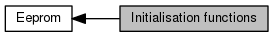
\includegraphics[width=277pt]{d7/d63/group___eeprom___init}
\end{center}
\end{figure}
\subsection*{Functions}
\begin{DoxyCompactItemize}
\item 
void \hyperlink{group___eeprom___init_ga4ec7f9d780da432051aa74ec5892a94c}{eeprom\+\_\+init} (void)
\begin{DoxyCompactList}\small\item\em Initialise communication to the eeprom. \end{DoxyCompactList}\end{DoxyCompactItemize}


\subsection{Detailed Description}
Eeprom initialisation functions. 



\subsection{Function Documentation}
\index{Initialisation functions@{Initialisation functions}!eeprom\+\_\+init@{eeprom\+\_\+init}}
\index{eeprom\+\_\+init@{eeprom\+\_\+init}!Initialisation functions@{Initialisation functions}}
\subsubsection[{\texorpdfstring{eeprom\+\_\+init(void)}{eeprom_init(void)}}]{\setlength{\rightskip}{0pt plus 5cm}void eeprom\+\_\+init (
\begin{DoxyParamCaption}
\item[{void}]{}
\end{DoxyParamCaption}
)}\hypertarget{group___eeprom___init_ga4ec7f9d780da432051aa74ec5892a94c}{}\label{group___eeprom___init_ga4ec7f9d780da432051aa74ec5892a94c}


Initialise communication to the eeprom. 


\begin{DoxyParams}{Parameters}
{\em None} & \\
\hline
\end{DoxyParams}

\begin{DoxyRetVals}{Return values}
{\em None} & \\
\hline
\end{DoxyRetVals}


Definition at line 48 of file N\+P\+C\+\_\+eeprom.\+c.



Here is the caller graph for this function\+:\nopagebreak
\begin{figure}[H]
\begin{center}
\leavevmode
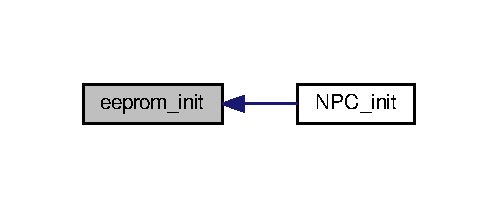
\includegraphics[width=239pt]{d7/d63/group___eeprom___init_ga4ec7f9d780da432051aa74ec5892a94c_icgraph}
\end{center}
\end{figure}



\hypertarget{group___eeprom___trans}{}\section{Transmission functions}
\label{group___eeprom___trans}\index{Transmission functions@{Transmission functions}}


Eeprom data transmission functions.  


Collaboration diagram for Transmission functions\+:\nopagebreak
\begin{figure}[H]
\begin{center}
\leavevmode
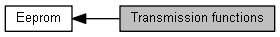
\includegraphics[width=284pt]{d2/de3/group___eeprom___trans}
\end{center}
\end{figure}
\subsection*{Functions}
\begin{DoxyCompactItemize}
\item 
Error\+Status \hyperlink{group___eeprom___trans_ga46c7b6081a89f96d53b6ebc0d0b6f60b}{eeprom\+\_\+write} (uint16\+\_\+t address, uint8\+\_\+t data)
\begin{DoxyCompactList}\small\item\em Write a byte to the eeprom. \end{DoxyCompactList}\item 
uint8\+\_\+t \hyperlink{group___eeprom___trans_gafaa7cca6f6ad1d9ae49522324c825c2f}{eeprom\+\_\+read} (uint16\+\_\+t address)
\begin{DoxyCompactList}\small\item\em Read a byte from the eeprom. \end{DoxyCompactList}\item 
Error\+Status \hyperlink{group___eeprom___trans_ga8c4d6169df1fdb9baeca667b5e9b0058}{eeprom\+\_\+write32\+Bytes} (uint16\+\_\+t base\+Address, uint8\+\_\+t $\ast$data)
\begin{DoxyCompactList}\small\item\em Write a page to the eeprom. \end{DoxyCompactList}\item 
uint32\+\_\+t \hyperlink{group___eeprom___trans_ga9a323370ddd02d91c6118f104c015b43}{eeprom\+\_\+read4\+Bytes} (uint16\+\_\+t base\+Address)
\begin{DoxyCompactList}\small\item\em Read a 32byte from eeprom. \end{DoxyCompactList}\item 
Error\+Status \hyperlink{group___eeprom___trans_ga9dea9d824339ffc184a047749533b96d}{eeprom\+\_\+write\+N\+Bytes} (uint16\+\_\+t base\+Address, uint8\+\_\+t $\ast$data, uint16\+\_\+t N)
\begin{DoxyCompactList}\small\item\em Write N bytes to the eeprom. \end{DoxyCompactList}\item 
Error\+Status \hyperlink{group___eeprom___trans_ga7d9db4a4822fa0c3e5b811615aaed569}{eeprom\+\_\+write4\+Bytes} (uint16\+\_\+t base\+Address, uint8\+\_\+t $\ast$data)
\begin{DoxyCompactList}\small\item\em Write 4 bytes to the eeprom. \end{DoxyCompactList}\item 
void \hyperlink{group___eeprom___trans_gab7c6abb0e0c39a8c152307fb822ffa0c}{eeprom\+\_\+read\+N\+Bytes} (uint16\+\_\+t base\+Address, uint8\+\_\+t $\ast$data, uint16\+\_\+t N)
\item 
void \hyperlink{group___eeprom___trans_ga7964a5a66da1c4a59a42309a93752217}{eeprom\+\_\+clear} (void)
\begin{DoxyCompactList}\small\item\em Clear eeprom data. \end{DoxyCompactList}\end{DoxyCompactItemize}


\subsection{Detailed Description}
Eeprom data transmission functions. 



\subsection{Function Documentation}
\index{Transmission functions@{Transmission functions}!eeprom\+\_\+clear@{eeprom\+\_\+clear}}
\index{eeprom\+\_\+clear@{eeprom\+\_\+clear}!Transmission functions@{Transmission functions}}
\subsubsection[{\texorpdfstring{eeprom\+\_\+clear(void)}{eeprom_clear(void)}}]{\setlength{\rightskip}{0pt plus 5cm}void eeprom\+\_\+clear (
\begin{DoxyParamCaption}
\item[{void}]{}
\end{DoxyParamCaption}
)}\hypertarget{group___eeprom___trans_ga7964a5a66da1c4a59a42309a93752217}{}\label{group___eeprom___trans_ga7964a5a66da1c4a59a42309a93752217}


Clear eeprom data. 


\begin{DoxyParams}{Parameters}
{\em None} & \\
\hline
\end{DoxyParams}

\begin{DoxyRetVals}{Return values}
{\em None} & \\
\hline
\end{DoxyRetVals}


Definition at line 242 of file N\+P\+C\+\_\+eeprom.\+c.



Here is the call graph for this function\+:\nopagebreak
\begin{figure}[H]
\begin{center}
\leavevmode
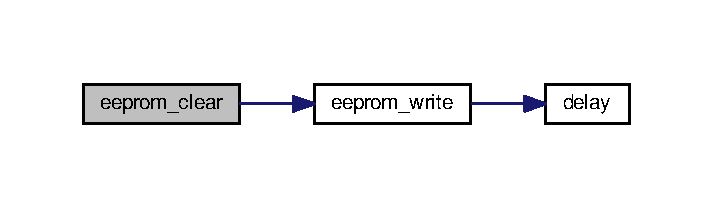
\includegraphics[width=342pt]{d2/de3/group___eeprom___trans_ga7964a5a66da1c4a59a42309a93752217_cgraph}
\end{center}
\end{figure}


\index{Transmission functions@{Transmission functions}!eeprom\+\_\+read@{eeprom\+\_\+read}}
\index{eeprom\+\_\+read@{eeprom\+\_\+read}!Transmission functions@{Transmission functions}}
\subsubsection[{\texorpdfstring{eeprom\+\_\+read(uint16\+\_\+t address)}{eeprom_read(uint16_t address)}}]{\setlength{\rightskip}{0pt plus 5cm}uint8\+\_\+t eeprom\+\_\+read (
\begin{DoxyParamCaption}
\item[{uint16\+\_\+t}]{address}
\end{DoxyParamCaption}
)}\hypertarget{group___eeprom___trans_gafaa7cca6f6ad1d9ae49522324c825c2f}{}\label{group___eeprom___trans_gafaa7cca6f6ad1d9ae49522324c825c2f}


Read a byte from the eeprom. 


\begin{DoxyParams}{Parameters}
{\em address} & The address of the memory \\
\hline
\end{DoxyParams}

\begin{DoxyRetVals}{Return values}
{\em uint8\+\_\+t} & data from eeprom \\
\hline
\end{DoxyRetVals}


Definition at line 156 of file N\+P\+C\+\_\+eeprom.\+c.



Here is the call graph for this function\+:\nopagebreak
\begin{figure}[H]
\begin{center}
\leavevmode
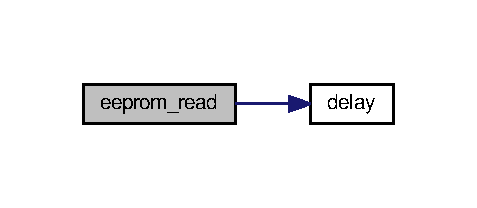
\includegraphics[width=229pt]{d2/de3/group___eeprom___trans_gafaa7cca6f6ad1d9ae49522324c825c2f_cgraph}
\end{center}
\end{figure}




Here is the caller graph for this function\+:
\nopagebreak
\begin{figure}[H]
\begin{center}
\leavevmode
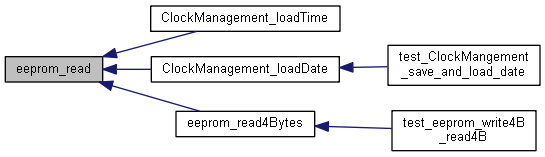
\includegraphics[width=350pt]{d2/de3/group___eeprom___trans_gafaa7cca6f6ad1d9ae49522324c825c2f_icgraph}
\end{center}
\end{figure}


\index{Transmission functions@{Transmission functions}!eeprom\+\_\+read4\+Bytes@{eeprom\+\_\+read4\+Bytes}}
\index{eeprom\+\_\+read4\+Bytes@{eeprom\+\_\+read4\+Bytes}!Transmission functions@{Transmission functions}}
\subsubsection[{\texorpdfstring{eeprom\+\_\+read4\+Bytes(uint16\+\_\+t base\+Address)}{eeprom_read4Bytes(uint16_t baseAddress)}}]{\setlength{\rightskip}{0pt plus 5cm}uint32\+\_\+t eeprom\+\_\+read4\+Bytes (
\begin{DoxyParamCaption}
\item[{uint16\+\_\+t}]{base\+Address}
\end{DoxyParamCaption}
)}\hypertarget{group___eeprom___trans_ga9a323370ddd02d91c6118f104c015b43}{}\label{group___eeprom___trans_ga9a323370ddd02d91c6118f104c015b43}


Read a 32byte from eeprom. 


\begin{DoxyParams}{Parameters}
{\em base\+Address} & \\
\hline
\end{DoxyParams}

\begin{DoxyRetVals}{Return values}
{\em uint32\+\_\+t} & \\
\hline
\end{DoxyRetVals}


Definition at line 295 of file N\+P\+C\+\_\+eeprom.\+c.



Here is the call graph for this function\+:\nopagebreak
\begin{figure}[H]
\begin{center}
\leavevmode
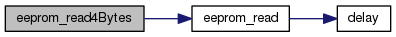
\includegraphics[width=350pt]{d2/de3/group___eeprom___trans_ga9a323370ddd02d91c6118f104c015b43_cgraph}
\end{center}
\end{figure}




Here is the caller graph for this function\+:\nopagebreak
\begin{figure}[H]
\begin{center}
\leavevmode
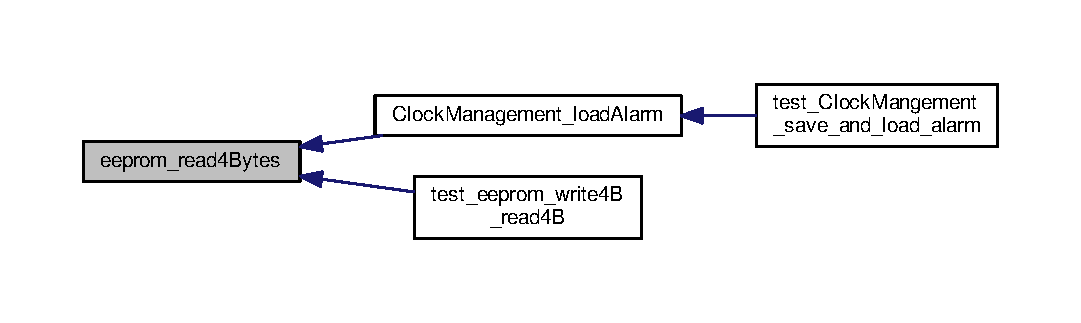
\includegraphics[width=350pt]{d2/de3/group___eeprom___trans_ga9a323370ddd02d91c6118f104c015b43_icgraph}
\end{center}
\end{figure}


\index{Transmission functions@{Transmission functions}!eeprom\+\_\+read\+N\+Bytes@{eeprom\+\_\+read\+N\+Bytes}}
\index{eeprom\+\_\+read\+N\+Bytes@{eeprom\+\_\+read\+N\+Bytes}!Transmission functions@{Transmission functions}}
\subsubsection[{\texorpdfstring{eeprom\+\_\+read\+N\+Bytes(uint16\+\_\+t base\+Address, uint8\+\_\+t $\ast$data, uint16\+\_\+t N)}{eeprom_readNBytes(uint16_t baseAddress, uint8_t *data, uint16_t N)}}]{\setlength{\rightskip}{0pt plus 5cm}void eeprom\+\_\+read\+N\+Bytes (
\begin{DoxyParamCaption}
\item[{uint16\+\_\+t}]{base\+Address, }
\item[{uint8\+\_\+t $\ast$}]{data, }
\item[{uint16\+\_\+t}]{N}
\end{DoxyParamCaption}
)}\hypertarget{group___eeprom___trans_gab7c6abb0e0c39a8c152307fb822ffa0c}{}\label{group___eeprom___trans_gab7c6abb0e0c39a8c152307fb822ffa0c}


Definition at line 309 of file N\+P\+C\+\_\+eeprom.\+c.



Here is the call graph for this function\+:
\nopagebreak
\begin{figure}[H]
\begin{center}
\leavevmode
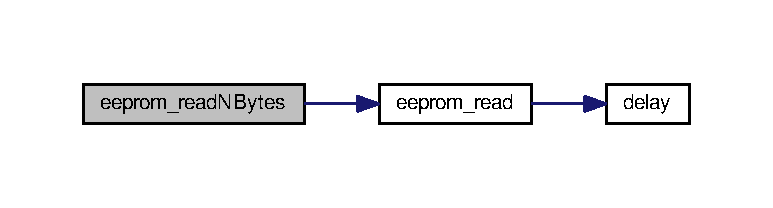
\includegraphics[width=350pt]{d2/de3/group___eeprom___trans_gab7c6abb0e0c39a8c152307fb822ffa0c_cgraph}
\end{center}
\end{figure}




Here is the caller graph for this function\+:
\nopagebreak
\begin{figure}[H]
\begin{center}
\leavevmode
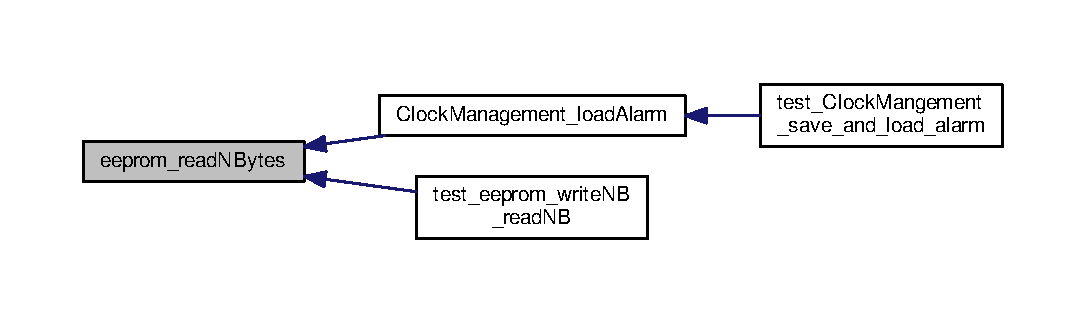
\includegraphics[width=350pt]{d2/de3/group___eeprom___trans_gab7c6abb0e0c39a8c152307fb822ffa0c_icgraph}
\end{center}
\end{figure}


\index{Transmission functions@{Transmission functions}!eeprom\+\_\+write@{eeprom\+\_\+write}}
\index{eeprom\+\_\+write@{eeprom\+\_\+write}!Transmission functions@{Transmission functions}}
\subsubsection[{\texorpdfstring{eeprom\+\_\+write(uint16\+\_\+t address, uint8\+\_\+t data)}{eeprom_write(uint16_t address, uint8_t data)}}]{\setlength{\rightskip}{0pt plus 5cm}Error\+Status eeprom\+\_\+write (
\begin{DoxyParamCaption}
\item[{uint16\+\_\+t}]{address, }
\item[{uint8\+\_\+t}]{data}
\end{DoxyParamCaption}
)}\hypertarget{group___eeprom___trans_ga46c7b6081a89f96d53b6ebc0d0b6f60b}{}\label{group___eeprom___trans_ga46c7b6081a89f96d53b6ebc0d0b6f60b}


Write a byte to the eeprom. 


\begin{DoxyParams}{Parameters}
{\em address} & The address of th memory \\
\hline
{\em data} & The data to be written to the memory \\
\hline
\end{DoxyParams}

\begin{DoxyRetVals}{Return values}
{\em None} & \\
\hline
\end{DoxyRetVals}


Definition at line 108 of file N\+P\+C\+\_\+eeprom.\+c.



Here is the call graph for this function\+:\nopagebreak
\begin{figure}[H]
\begin{center}
\leavevmode
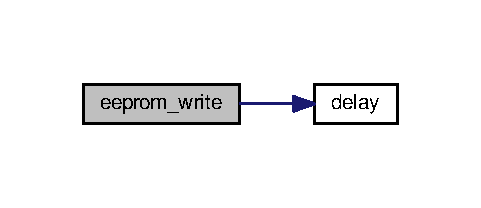
\includegraphics[width=231pt]{d2/de3/group___eeprom___trans_ga46c7b6081a89f96d53b6ebc0d0b6f60b_cgraph}
\end{center}
\end{figure}




Here is the caller graph for this function\+:
\nopagebreak
\begin{figure}[H]
\begin{center}
\leavevmode
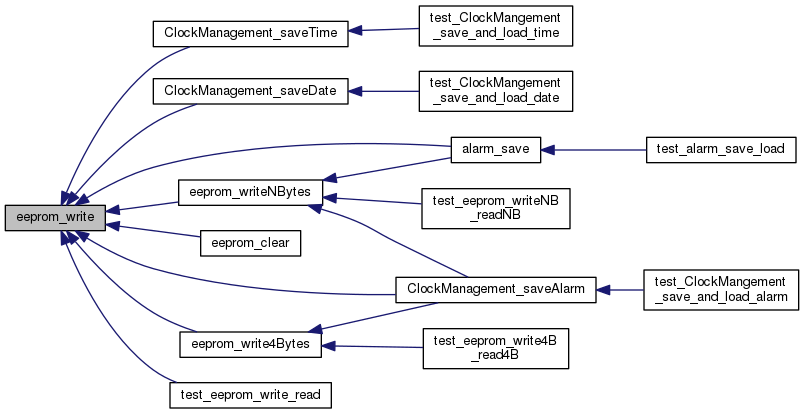
\includegraphics[width=350pt]{d2/de3/group___eeprom___trans_ga46c7b6081a89f96d53b6ebc0d0b6f60b_icgraph}
\end{center}
\end{figure}


\index{Transmission functions@{Transmission functions}!eeprom\+\_\+write32\+Bytes@{eeprom\+\_\+write32\+Bytes}}
\index{eeprom\+\_\+write32\+Bytes@{eeprom\+\_\+write32\+Bytes}!Transmission functions@{Transmission functions}}
\subsubsection[{\texorpdfstring{eeprom\+\_\+write32\+Bytes(uint16\+\_\+t base\+Address, uint8\+\_\+t $\ast$data)}{eeprom_write32Bytes(uint16_t baseAddress, uint8_t *data)}}]{\setlength{\rightskip}{0pt plus 5cm}Error\+Status eeprom\+\_\+write32\+Bytes (
\begin{DoxyParamCaption}
\item[{uint16\+\_\+t}]{base\+Address, }
\item[{uint8\+\_\+t $\ast$}]{data}
\end{DoxyParamCaption}
)}\hypertarget{group___eeprom___trans_ga8c4d6169df1fdb9baeca667b5e9b0058}{}\label{group___eeprom___trans_ga8c4d6169df1fdb9baeca667b5e9b0058}


Write a page to the eeprom. 


\begin{DoxyParams}{Parameters}
{\em base\+Address} & The base address of the page \\
\hline
{\em data} & An array of data to be send \\
\hline
\end{DoxyParams}

\begin{DoxyRetVals}{Return values}
{\em None} & \\
\hline
\end{DoxyRetVals}


Definition at line 192 of file N\+P\+C\+\_\+eeprom.\+c.



Here is the call graph for this function\+:\nopagebreak
\begin{figure}[H]
\begin{center}
\leavevmode
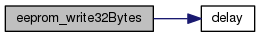
\includegraphics[width=267pt]{d2/de3/group___eeprom___trans_ga8c4d6169df1fdb9baeca667b5e9b0058_cgraph}
\end{center}
\end{figure}




Here is the caller graph for this function\+:\nopagebreak
\begin{figure}[H]
\begin{center}
\leavevmode
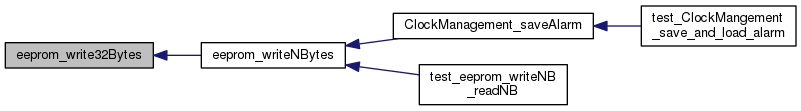
\includegraphics[width=350pt]{d2/de3/group___eeprom___trans_ga8c4d6169df1fdb9baeca667b5e9b0058_icgraph}
\end{center}
\end{figure}


\index{Transmission functions@{Transmission functions}!eeprom\+\_\+write4\+Bytes@{eeprom\+\_\+write4\+Bytes}}
\index{eeprom\+\_\+write4\+Bytes@{eeprom\+\_\+write4\+Bytes}!Transmission functions@{Transmission functions}}
\subsubsection[{\texorpdfstring{eeprom\+\_\+write4\+Bytes(uint16\+\_\+t base\+Address, uint8\+\_\+t $\ast$data)}{eeprom_write4Bytes(uint16_t baseAddress, uint8_t *data)}}]{\setlength{\rightskip}{0pt plus 5cm}Error\+Status eeprom\+\_\+write4\+Bytes (
\begin{DoxyParamCaption}
\item[{uint16\+\_\+t}]{base\+Address, }
\item[{uint8\+\_\+t $\ast$}]{data}
\end{DoxyParamCaption}
)}\hypertarget{group___eeprom___trans_ga7d9db4a4822fa0c3e5b811615aaed569}{}\label{group___eeprom___trans_ga7d9db4a4822fa0c3e5b811615aaed569}


Write 4 bytes to the eeprom. 


\begin{DoxyParams}{Parameters}
{\em base\+Address} & address of data \\
\hline
{\em data} & data to be written \\
\hline
\end{DoxyParams}

\begin{DoxyRetVals}{Return values}
{\em Error\+Status} & \\
\hline
\end{DoxyRetVals}


Definition at line 279 of file N\+P\+C\+\_\+eeprom.\+c.



Here is the call graph for this function\+:\nopagebreak
\begin{figure}[H]
\begin{center}
\leavevmode
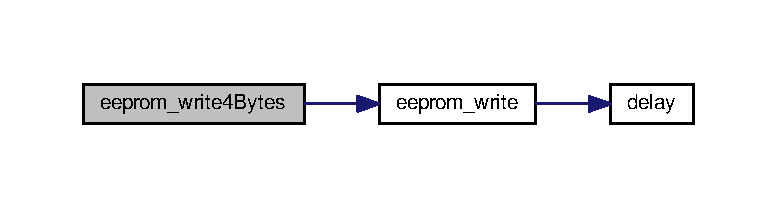
\includegraphics[width=350pt]{d2/de3/group___eeprom___trans_ga7d9db4a4822fa0c3e5b811615aaed569_cgraph}
\end{center}
\end{figure}




Here is the caller graph for this function\+:\nopagebreak
\begin{figure}[H]
\begin{center}
\leavevmode
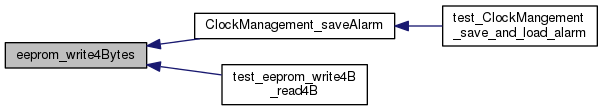
\includegraphics[width=350pt]{d2/de3/group___eeprom___trans_ga7d9db4a4822fa0c3e5b811615aaed569_icgraph}
\end{center}
\end{figure}


\index{Transmission functions@{Transmission functions}!eeprom\+\_\+write\+N\+Bytes@{eeprom\+\_\+write\+N\+Bytes}}
\index{eeprom\+\_\+write\+N\+Bytes@{eeprom\+\_\+write\+N\+Bytes}!Transmission functions@{Transmission functions}}
\subsubsection[{\texorpdfstring{eeprom\+\_\+write\+N\+Bytes(uint16\+\_\+t base\+Address, uint8\+\_\+t $\ast$data, uint16\+\_\+t N)}{eeprom_writeNBytes(uint16_t baseAddress, uint8_t *data, uint16_t N)}}]{\setlength{\rightskip}{0pt plus 5cm}Error\+Status eeprom\+\_\+write\+N\+Bytes (
\begin{DoxyParamCaption}
\item[{uint16\+\_\+t}]{base\+Address, }
\item[{uint8\+\_\+t $\ast$}]{data, }
\item[{uint16\+\_\+t}]{N}
\end{DoxyParamCaption}
)}\hypertarget{group___eeprom___trans_ga9dea9d824339ffc184a047749533b96d}{}\label{group___eeprom___trans_ga9dea9d824339ffc184a047749533b96d}


Write N bytes to the eeprom. 

\begin{DoxyNote}{Note}
N is divided into pages before been written to memory 
\end{DoxyNote}

\begin{DoxyParams}{Parameters}
{\em base\+Address} & address of data \\
\hline
{\em data} & data to be written \\
\hline
{\em N} & number of data to write \\
\hline
\end{DoxyParams}

\begin{DoxyRetVals}{Return values}
{\em Error\+Status} & \\
\hline
\end{DoxyRetVals}


Definition at line 259 of file N\+P\+C\+\_\+eeprom.\+c.



Here is the call graph for this function\+:\nopagebreak
\begin{figure}[H]
\begin{center}
\leavevmode
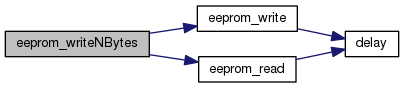
\includegraphics[width=350pt]{d2/de3/group___eeprom___trans_ga9dea9d824339ffc184a047749533b96d_cgraph}
\end{center}
\end{figure}




Here is the caller graph for this function\+:\nopagebreak
\begin{figure}[H]
\begin{center}
\leavevmode
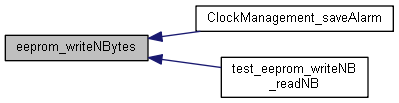
\includegraphics[width=350pt]{d2/de3/group___eeprom___trans_ga9dea9d824339ffc184a047749533b96d_icgraph}
\end{center}
\end{figure}



\hypertarget{group___neo_pixel}{}\section{Neo\+Pixel}
\label{group___neo_pixel}\index{Neo\+Pixel@{Neo\+Pixel}}


neopixel driver modules  


\subsection*{Modules}
\begin{DoxyCompactItemize}
\item 
\hyperlink{group___constant}{Constant}
\begin{DoxyCompactList}\small\item\em Define audio frequency and D\+MA frequency. \end{DoxyCompactList}\item 
\hyperlink{group___neo_pixel___init}{Initialisation functions}
\begin{DoxyCompactList}\small\item\em Neopixel initialisation functions. \end{DoxyCompactList}\item 
\hyperlink{group___neo_pixel___state}{State alteration functions}
\begin{DoxyCompactList}\small\item\em Neopixel state alteration functions. \end{DoxyCompactList}\item 
\hyperlink{group___neo_pixel___colour}{Colour generation functions}
\begin{DoxyCompactList}\small\item\em Neopixel colour functions. \end{DoxyCompactList}\item 
\hyperlink{group___neo_pixel___display}{colour display functions}
\begin{DoxyCompactList}\small\item\em Neopixel colour display functions. \end{DoxyCompactList}\end{DoxyCompactItemize}
\subsection*{Functions}
\begin{DoxyCompactItemize}
\item 
void \hyperlink{group___neo_pixel_gaac78468985e44a3e4d353ea9276b33bc}{neopixel\+\_\+init} (void)
\begin{DoxyCompactList}\small\item\em Initialise the neopixel. \end{DoxyCompactList}\item 
void \hyperlink{group___neo_pixel_gae027558106eef5c81996294f4561fecb}{neopixel\+\_\+set\+Brightness} (uint8\+\_\+t b)
\begin{DoxyCompactList}\small\item\em Set the brightness of the led. \end{DoxyCompactList}\item 
\mbox{\Hypertarget{group___neo_pixel_gada44b0356745943702c92d394760cd3e}\label{group___neo_pixel_gada44b0356745943702c92d394760cd3e}} 
void {\bfseries neopixel\+\_\+set\+State} (uint8\+\_\+t s)
\item 
\mbox{\Hypertarget{group___neo_pixel_gadb692027c25b23852a28f2ca43dc2399}\label{group___neo_pixel_gadb692027c25b23852a28f2ca43dc2399}} 
void {\bfseries neopixel\+\_\+show} (void)
\item 
void \hyperlink{group___neo_pixel_ga8e3cfef785ce221672f825f8785c25b8}{neopixel\+\_\+clear} (void)
\begin{DoxyCompactList}\small\item\em Stop pushing data to the neopixels. \end{DoxyCompactList}\item 
void \hyperlink{group___neo_pixel_ga79e34feddcfb2c45ae218166c84bdff4}{neopixel\+\_\+data\+Init} (void)
\begin{DoxyCompactList}\small\item\em Initialise the L\+E\+Dbuffer. \end{DoxyCompactList}\item 
void \hyperlink{group___neo_pixel_ga38ad4725462bdc5e86c4ead4f04b9fc2}{T\+I\+M2\+\_\+\+I\+R\+Q\+Handler} (void)
\begin{DoxyCompactList}\small\item\em Timer Handler for neopixel. \end{DoxyCompactList}\item 
uint32\+\_\+t \hyperlink{group___neo_pixel_ga1d500fbcbecad76feef8835437687ca0}{neopixel\+\_\+colour\+R\+GB} (uint8\+\_\+t r, uint8\+\_\+t g, uint8\+\_\+t b)
\begin{DoxyCompactList}\small\item\em convert R\+GB 3 8bit colour to a 32bit colour \end{DoxyCompactList}\item 
uint32\+\_\+t \hyperlink{group___neo_pixel_ga527ba03b45a249e5e1ea1da4b971b3ac}{neopixel\+\_\+colour\+R\+G\+BW} (uint8\+\_\+t r, uint8\+\_\+t g, uint8\+\_\+t b, uint8\+\_\+t w)
\begin{DoxyCompactList}\small\item\em convert R\+GB 3 8bit colour to a 32bit colour \end{DoxyCompactList}\item 
void \hyperlink{group___neo_pixel_ga63c196a71ffb007411929e41ba5df41d}{neopixel\+\_\+set\+Pixel\+Colour\+R\+GB} (uint8\+\_\+t n, uint8\+\_\+t r, uint8\+\_\+t g, uint8\+\_\+t b)
\begin{DoxyCompactList}\small\item\em Set the colour of one led. \end{DoxyCompactList}\item 
void \hyperlink{group___neo_pixel_ga58d5ceb79029ca8dc5dd8b27b65e4f09}{neopixel\+\_\+set\+Pixel\+Colour\+R\+G\+BW} (uint8\+\_\+t n, uint8\+\_\+t r, uint8\+\_\+t g, uint8\+\_\+t b, uint8\+\_\+t w)
\begin{DoxyCompactList}\small\item\em Set the colour of one led. \end{DoxyCompactList}\item 
void \hyperlink{group___neo_pixel_gaecbdecac1da356c5fba07058983d9066}{neopixel\+\_\+set\+Pixel\+Colour} (uint8\+\_\+t n, uint32\+\_\+t c)
\begin{DoxyCompactList}\small\item\em Set the colour of one led. \end{DoxyCompactList}\item 
void \hyperlink{group___neo_pixel_ga4daf6edfe83394f425ec51f64d92c49c}{neopixel\+\_\+set\+Pixel\+ColourW} (uint8\+\_\+t n, uint32\+\_\+t c)
\begin{DoxyCompactList}\small\item\em Set the colour of one led. \end{DoxyCompactList}\item 
void \hyperlink{group___neo_pixel_ga7a6c2dc149e86a788aede1d6aa5262d7}{neopixel\+\_\+set\+All\+Pixel\+R\+GB} (uint8\+\_\+t r, uint8\+\_\+t g, uint8\+\_\+t b)
\begin{DoxyCompactList}\small\item\em set all the pixel on the line to a specific colour \end{DoxyCompactList}\item 
void \hyperlink{group___neo_pixel_ga1ba017c1f338ef2c8e4a48acae35d87e}{neopixel\+\_\+set\+All\+Pixel\+R\+G\+BW} (uint8\+\_\+t r, uint8\+\_\+t g, uint8\+\_\+t b, uint8\+\_\+t w)
\begin{DoxyCompactList}\small\item\em set all the pixel on the line to a specific colour \end{DoxyCompactList}\end{DoxyCompactItemize}


\subsection{Detailed Description}
neopixel driver modules 



\subsection{Function Documentation}
\mbox{\Hypertarget{group___neo_pixel_ga8e3cfef785ce221672f825f8785c25b8}\label{group___neo_pixel_ga8e3cfef785ce221672f825f8785c25b8}} 
\index{Neo\+Pixel@{Neo\+Pixel}!neopixel\+\_\+clear@{neopixel\+\_\+clear}}
\index{neopixel\+\_\+clear@{neopixel\+\_\+clear}!Neo\+Pixel@{Neo\+Pixel}}
\subsubsection{\texorpdfstring{neopixel\+\_\+clear()}{neopixel\_clear()}}
{\footnotesize\ttfamily void neopixel\+\_\+clear (\begin{DoxyParamCaption}\item[{void}]{ }\end{DoxyParamCaption})}



Stop pushing data to the neopixels. 


\begin{DoxyParams}{Parameters}
{\em None} & \\
\hline
\end{DoxyParams}

\begin{DoxyRetVals}{Return values}
{\em None} & \\
\hline
\end{DoxyRetVals}
\mbox{\Hypertarget{group___neo_pixel_ga1d500fbcbecad76feef8835437687ca0}\label{group___neo_pixel_ga1d500fbcbecad76feef8835437687ca0}} 
\index{Neo\+Pixel@{Neo\+Pixel}!neopixel\+\_\+colour\+R\+GB@{neopixel\+\_\+colour\+R\+GB}}
\index{neopixel\+\_\+colour\+R\+GB@{neopixel\+\_\+colour\+R\+GB}!Neo\+Pixel@{Neo\+Pixel}}
\subsubsection{\texorpdfstring{neopixel\+\_\+colour\+R\+G\+B()}{neopixel\_colourRGB()}}
{\footnotesize\ttfamily uint32\+\_\+t neopixel\+\_\+colour\+R\+GB (\begin{DoxyParamCaption}\item[{uint8\+\_\+t}]{r,  }\item[{uint8\+\_\+t}]{g,  }\item[{uint8\+\_\+t}]{b }\end{DoxyParamCaption})}



convert R\+GB 3 8bit colour to a 32bit colour 

\begin{DoxyNote}{Note}
M\+S3 0, M\+S2 r, M\+S1 g, M\+S0 b 
\end{DoxyNote}

\begin{DoxyParams}{Parameters}
{\em r} & R\+ED intensity \\
\hline
{\em g} & G\+R\+E\+EN intensity \\
\hline
{\em b} & B\+L\+UE intensity \\
\hline
\end{DoxyParams}

\begin{DoxyRetVals}{Return values}
{\em None} & \\
\hline
\end{DoxyRetVals}
\mbox{\Hypertarget{group___neo_pixel_ga527ba03b45a249e5e1ea1da4b971b3ac}\label{group___neo_pixel_ga527ba03b45a249e5e1ea1da4b971b3ac}} 
\index{Neo\+Pixel@{Neo\+Pixel}!neopixel\+\_\+colour\+R\+G\+BW@{neopixel\+\_\+colour\+R\+G\+BW}}
\index{neopixel\+\_\+colour\+R\+G\+BW@{neopixel\+\_\+colour\+R\+G\+BW}!Neo\+Pixel@{Neo\+Pixel}}
\subsubsection{\texorpdfstring{neopixel\+\_\+colour\+R\+G\+B\+W()}{neopixel\_colourRGBW()}}
{\footnotesize\ttfamily uint32\+\_\+t neopixel\+\_\+colour\+R\+G\+BW (\begin{DoxyParamCaption}\item[{uint8\+\_\+t}]{r,  }\item[{uint8\+\_\+t}]{g,  }\item[{uint8\+\_\+t}]{b,  }\item[{uint8\+\_\+t}]{w }\end{DoxyParamCaption})}



convert R\+GB 3 8bit colour to a 32bit colour 

\begin{DoxyNote}{Note}
M\+S3 w, M\+S2 r, M\+S1 g, M\+S0 b 
\end{DoxyNote}

\begin{DoxyParams}{Parameters}
{\em r} & R\+ED intensity \\
\hline
{\em g} & G\+R\+E\+EN intensity \\
\hline
{\em b} & B\+L\+UE intensity \\
\hline
{\em w} & W\+H\+I\+TE intensity \\
\hline
\end{DoxyParams}

\begin{DoxyRetVals}{Return values}
{\em None} & \\
\hline
\end{DoxyRetVals}
\mbox{\Hypertarget{group___neo_pixel_ga79e34feddcfb2c45ae218166c84bdff4}\label{group___neo_pixel_ga79e34feddcfb2c45ae218166c84bdff4}} 
\index{Neo\+Pixel@{Neo\+Pixel}!neopixel\+\_\+data\+Init@{neopixel\+\_\+data\+Init}}
\index{neopixel\+\_\+data\+Init@{neopixel\+\_\+data\+Init}!Neo\+Pixel@{Neo\+Pixel}}
\subsubsection{\texorpdfstring{neopixel\+\_\+data\+Init()}{neopixel\_dataInit()}}
{\footnotesize\ttfamily void neopixel\+\_\+data\+Init (\begin{DoxyParamCaption}\item[{void}]{ }\end{DoxyParamCaption})}



Initialise the L\+E\+Dbuffer. 


\begin{DoxyParams}{Parameters}
{\em None} & \\
\hline
\end{DoxyParams}

\begin{DoxyRetVals}{Return values}
{\em None} & \\
\hline
\end{DoxyRetVals}
\mbox{\Hypertarget{group___neo_pixel_gaac78468985e44a3e4d353ea9276b33bc}\label{group___neo_pixel_gaac78468985e44a3e4d353ea9276b33bc}} 
\index{Neo\+Pixel@{Neo\+Pixel}!neopixel\+\_\+init@{neopixel\+\_\+init}}
\index{neopixel\+\_\+init@{neopixel\+\_\+init}!Neo\+Pixel@{Neo\+Pixel}}
\subsubsection{\texorpdfstring{neopixel\+\_\+init()}{neopixel\_init()}}
{\footnotesize\ttfamily void neopixel\+\_\+init (\begin{DoxyParamCaption}\item[{void}]{ }\end{DoxyParamCaption})}



Initialise the neopixel. 


\begin{DoxyParams}{Parameters}
{\em None} & \\
\hline
\end{DoxyParams}

\begin{DoxyRetVals}{Return values}
{\em None} & \\
\hline
\end{DoxyRetVals}
\mbox{\Hypertarget{group___neo_pixel_ga7a6c2dc149e86a788aede1d6aa5262d7}\label{group___neo_pixel_ga7a6c2dc149e86a788aede1d6aa5262d7}} 
\index{Neo\+Pixel@{Neo\+Pixel}!neopixel\+\_\+set\+All\+Pixel\+R\+GB@{neopixel\+\_\+set\+All\+Pixel\+R\+GB}}
\index{neopixel\+\_\+set\+All\+Pixel\+R\+GB@{neopixel\+\_\+set\+All\+Pixel\+R\+GB}!Neo\+Pixel@{Neo\+Pixel}}
\subsubsection{\texorpdfstring{neopixel\+\_\+set\+All\+Pixel\+R\+G\+B()}{neopixel\_setAllPixelRGB()}}
{\footnotesize\ttfamily void neopixel\+\_\+set\+All\+Pixel\+R\+GB (\begin{DoxyParamCaption}\item[{uint8\+\_\+t}]{r,  }\item[{uint8\+\_\+t}]{g,  }\item[{uint8\+\_\+t}]{b }\end{DoxyParamCaption})}



set all the pixel on the line to a specific colour 


\begin{DoxyParams}{Parameters}
{\em r} & R\+ED intensity \\
\hline
{\em g} & G\+R\+E\+EN intensity \\
\hline
{\em b} & B\+L\+UE intensity \\
\hline
\end{DoxyParams}

\begin{DoxyRetVals}{Return values}
{\em None} & \\
\hline
\end{DoxyRetVals}
\mbox{\Hypertarget{group___neo_pixel_ga1ba017c1f338ef2c8e4a48acae35d87e}\label{group___neo_pixel_ga1ba017c1f338ef2c8e4a48acae35d87e}} 
\index{Neo\+Pixel@{Neo\+Pixel}!neopixel\+\_\+set\+All\+Pixel\+R\+G\+BW@{neopixel\+\_\+set\+All\+Pixel\+R\+G\+BW}}
\index{neopixel\+\_\+set\+All\+Pixel\+R\+G\+BW@{neopixel\+\_\+set\+All\+Pixel\+R\+G\+BW}!Neo\+Pixel@{Neo\+Pixel}}
\subsubsection{\texorpdfstring{neopixel\+\_\+set\+All\+Pixel\+R\+G\+B\+W()}{neopixel\_setAllPixelRGBW()}}
{\footnotesize\ttfamily void neopixel\+\_\+set\+All\+Pixel\+R\+G\+BW (\begin{DoxyParamCaption}\item[{uint8\+\_\+t}]{r,  }\item[{uint8\+\_\+t}]{g,  }\item[{uint8\+\_\+t}]{b,  }\item[{uint8\+\_\+t}]{w }\end{DoxyParamCaption})}



set all the pixel on the line to a specific colour 


\begin{DoxyParams}{Parameters}
{\em r} & R\+ED intensity \\
\hline
{\em g} & G\+R\+E\+EN intensity \\
\hline
{\em b} & B\+L\+UE intensity \\
\hline
{\em w} & W\+H\+I\+TE intensity \\
\hline
\end{DoxyParams}

\begin{DoxyRetVals}{Return values}
{\em None} & \\
\hline
\end{DoxyRetVals}
\mbox{\Hypertarget{group___neo_pixel_gae027558106eef5c81996294f4561fecb}\label{group___neo_pixel_gae027558106eef5c81996294f4561fecb}} 
\index{Neo\+Pixel@{Neo\+Pixel}!neopixel\+\_\+set\+Brightness@{neopixel\+\_\+set\+Brightness}}
\index{neopixel\+\_\+set\+Brightness@{neopixel\+\_\+set\+Brightness}!Neo\+Pixel@{Neo\+Pixel}}
\subsubsection{\texorpdfstring{neopixel\+\_\+set\+Brightness()}{neopixel\_setBrightness()}}
{\footnotesize\ttfamily void neopixel\+\_\+set\+Brightness (\begin{DoxyParamCaption}\item[{uint8\+\_\+t}]{b }\end{DoxyParamCaption})}



Set the brightness of the led. 

\begin{DoxyNote}{Note}
-\/ completely dim\+: 0
\begin{DoxyItemize}
\item fully bright\+: 255 
\end{DoxyItemize}
\end{DoxyNote}

\begin{DoxyParams}{Parameters}
{\em b} & Brightness \\
\hline
\end{DoxyParams}

\begin{DoxyRetVals}{Return values}
{\em None} & \\
\hline
\end{DoxyRetVals}
\mbox{\Hypertarget{group___neo_pixel_gaecbdecac1da356c5fba07058983d9066}\label{group___neo_pixel_gaecbdecac1da356c5fba07058983d9066}} 
\index{Neo\+Pixel@{Neo\+Pixel}!neopixel\+\_\+set\+Pixel\+Colour@{neopixel\+\_\+set\+Pixel\+Colour}}
\index{neopixel\+\_\+set\+Pixel\+Colour@{neopixel\+\_\+set\+Pixel\+Colour}!Neo\+Pixel@{Neo\+Pixel}}
\subsubsection{\texorpdfstring{neopixel\+\_\+set\+Pixel\+Colour()}{neopixel\_setPixelColour()}}
{\footnotesize\ttfamily void neopixel\+\_\+set\+Pixel\+Colour (\begin{DoxyParamCaption}\item[{uint8\+\_\+t}]{n,  }\item[{uint32\+\_\+t}]{c }\end{DoxyParamCaption})}



Set the colour of one led. 


\begin{DoxyParams}{Parameters}
{\em n} & Led index \\
\hline
{\em c} & 32bit R\+GB colour \\
\hline
\end{DoxyParams}

\begin{DoxyRetVals}{Return values}
{\em None} & \\
\hline
\end{DoxyRetVals}
\mbox{\Hypertarget{group___neo_pixel_ga63c196a71ffb007411929e41ba5df41d}\label{group___neo_pixel_ga63c196a71ffb007411929e41ba5df41d}} 
\index{Neo\+Pixel@{Neo\+Pixel}!neopixel\+\_\+set\+Pixel\+Colour\+R\+GB@{neopixel\+\_\+set\+Pixel\+Colour\+R\+GB}}
\index{neopixel\+\_\+set\+Pixel\+Colour\+R\+GB@{neopixel\+\_\+set\+Pixel\+Colour\+R\+GB}!Neo\+Pixel@{Neo\+Pixel}}
\subsubsection{\texorpdfstring{neopixel\+\_\+set\+Pixel\+Colour\+R\+G\+B()}{neopixel\_setPixelColourRGB()}}
{\footnotesize\ttfamily void neopixel\+\_\+set\+Pixel\+Colour\+R\+GB (\begin{DoxyParamCaption}\item[{uint8\+\_\+t}]{n,  }\item[{uint8\+\_\+t}]{r,  }\item[{uint8\+\_\+t}]{g,  }\item[{uint8\+\_\+t}]{b }\end{DoxyParamCaption})}



Set the colour of one led. 


\begin{DoxyParams}{Parameters}
{\em n} & Led index \\
\hline
{\em r} & R\+ED intensity \\
\hline
{\em g} & G\+R\+E\+EN intensity \\
\hline
{\em b} & B\+L\+UE intensity \\
\hline
\end{DoxyParams}

\begin{DoxyRetVals}{Return values}
{\em None} & \\
\hline
\end{DoxyRetVals}
\mbox{\Hypertarget{group___neo_pixel_ga58d5ceb79029ca8dc5dd8b27b65e4f09}\label{group___neo_pixel_ga58d5ceb79029ca8dc5dd8b27b65e4f09}} 
\index{Neo\+Pixel@{Neo\+Pixel}!neopixel\+\_\+set\+Pixel\+Colour\+R\+G\+BW@{neopixel\+\_\+set\+Pixel\+Colour\+R\+G\+BW}}
\index{neopixel\+\_\+set\+Pixel\+Colour\+R\+G\+BW@{neopixel\+\_\+set\+Pixel\+Colour\+R\+G\+BW}!Neo\+Pixel@{Neo\+Pixel}}
\subsubsection{\texorpdfstring{neopixel\+\_\+set\+Pixel\+Colour\+R\+G\+B\+W()}{neopixel\_setPixelColourRGBW()}}
{\footnotesize\ttfamily void neopixel\+\_\+set\+Pixel\+Colour\+R\+G\+BW (\begin{DoxyParamCaption}\item[{uint8\+\_\+t}]{n,  }\item[{uint8\+\_\+t}]{r,  }\item[{uint8\+\_\+t}]{g,  }\item[{uint8\+\_\+t}]{b,  }\item[{uint8\+\_\+t}]{w }\end{DoxyParamCaption})}



Set the colour of one led. 


\begin{DoxyParams}{Parameters}
{\em n} & Led index \\
\hline
{\em r} & R\+ED intensity \\
\hline
{\em g} & G\+R\+E\+EN intensity \\
\hline
{\em b} & B\+L\+UE intensity \\
\hline
{\em w} & W\+H\+I\+TE intensity \\
\hline
\end{DoxyParams}

\begin{DoxyRetVals}{Return values}
{\em None} & \\
\hline
\end{DoxyRetVals}
\mbox{\Hypertarget{group___neo_pixel_ga4daf6edfe83394f425ec51f64d92c49c}\label{group___neo_pixel_ga4daf6edfe83394f425ec51f64d92c49c}} 
\index{Neo\+Pixel@{Neo\+Pixel}!neopixel\+\_\+set\+Pixel\+ColourW@{neopixel\+\_\+set\+Pixel\+ColourW}}
\index{neopixel\+\_\+set\+Pixel\+ColourW@{neopixel\+\_\+set\+Pixel\+ColourW}!Neo\+Pixel@{Neo\+Pixel}}
\subsubsection{\texorpdfstring{neopixel\+\_\+set\+Pixel\+Colour\+W()}{neopixel\_setPixelColourW()}}
{\footnotesize\ttfamily void neopixel\+\_\+set\+Pixel\+ColourW (\begin{DoxyParamCaption}\item[{uint8\+\_\+t}]{n,  }\item[{uint32\+\_\+t}]{c }\end{DoxyParamCaption})}



Set the colour of one led. 


\begin{DoxyParams}{Parameters}
{\em n} & Led index \\
\hline
{\em c} & 32bit R\+GB colour \\
\hline
\end{DoxyParams}

\begin{DoxyRetVals}{Return values}
{\em None} & \\
\hline
\end{DoxyRetVals}
\mbox{\Hypertarget{group___neo_pixel_ga38ad4725462bdc5e86c4ead4f04b9fc2}\label{group___neo_pixel_ga38ad4725462bdc5e86c4ead4f04b9fc2}} 
\index{Neo\+Pixel@{Neo\+Pixel}!T\+I\+M2\+\_\+\+I\+R\+Q\+Handler@{T\+I\+M2\+\_\+\+I\+R\+Q\+Handler}}
\index{T\+I\+M2\+\_\+\+I\+R\+Q\+Handler@{T\+I\+M2\+\_\+\+I\+R\+Q\+Handler}!Neo\+Pixel@{Neo\+Pixel}}
\subsubsection{\texorpdfstring{T\+I\+M2\+\_\+\+I\+R\+Q\+Handler()}{TIM2\_IRQHandler()}}
{\footnotesize\ttfamily void T\+I\+M2\+\_\+\+I\+R\+Q\+Handler (\begin{DoxyParamCaption}\item[{void}]{ }\end{DoxyParamCaption})}



Timer Handler for neopixel. 

\begin{DoxyNote}{Note}
L\+E\+D\+Buffer is pushed every time the handle is called 
\end{DoxyNote}

\begin{DoxyParams}{Parameters}
{\em None} & \\
\hline
\end{DoxyParams}

\begin{DoxyRetVals}{Return values}
{\em None} & \\
\hline
\end{DoxyRetVals}

\hypertarget{group___neo_pixel___init}{}\section{Initialisation functions}
\label{group___neo_pixel___init}\index{Initialisation functions@{Initialisation functions}}


Neopixel initialisation functions.  


Collaboration diagram for Initialisation functions\+:
% FIG 0
\subsection*{Functions}
\begin{DoxyCompactItemize}
\item 
void \hyperlink{group___neo_pixel___init_gaac78468985e44a3e4d353ea9276b33bc}{neopixel\+\_\+init} (void)
\begin{DoxyCompactList}\small\item\em Initialise the neopixel. \end{DoxyCompactList}\end{DoxyCompactItemize}


\subsection{Detailed Description}
Neopixel initialisation functions. 



\subsection{Function Documentation}
\mbox{\Hypertarget{group___neo_pixel___init_gaac78468985e44a3e4d353ea9276b33bc}\label{group___neo_pixel___init_gaac78468985e44a3e4d353ea9276b33bc}} 
\index{Initialisation functions@{Initialisation functions}!neopixel\+\_\+init@{neopixel\+\_\+init}}
\index{neopixel\+\_\+init@{neopixel\+\_\+init}!Initialisation functions@{Initialisation functions}}
\subsubsection{\texorpdfstring{neopixel\+\_\+init()}{neopixel\_init()}}
{\footnotesize\ttfamily void neopixel\+\_\+init (\begin{DoxyParamCaption}\item[{void}]{ }\end{DoxyParamCaption})}



Initialise the neopixel. 


\begin{DoxyParams}{Parameters}
{\em None} & \\
\hline
\end{DoxyParams}

\begin{DoxyRetVals}{Return values}
{\em None} & \\
\hline
\end{DoxyRetVals}

\hypertarget{group___neo_pixel___state}{}\section{State alteration functions}
\label{group___neo_pixel___state}\index{State alteration functions@{State alteration functions}}


Neopixel state alteration functions.  


Collaboration diagram for State alteration functions\+:
% FIG 0
\subsection*{Functions}
\begin{DoxyCompactItemize}
\item 
void \hyperlink{group___neo_pixel___state_ga38ad4725462bdc5e86c4ead4f04b9fc2}{T\+I\+M2\+\_\+\+I\+R\+Q\+Handler} (void)
\begin{DoxyCompactList}\small\item\em Timer Handler for neopixel. \end{DoxyCompactList}\item 
void \hyperlink{group___neo_pixel___state_ga8e3cfef785ce221672f825f8785c25b8}{neopixel\+\_\+clear} (void)
\begin{DoxyCompactList}\small\item\em Stop pushing data to the neopixels. \end{DoxyCompactList}\item 
void \hyperlink{group___neo_pixel___state_ga79e34feddcfb2c45ae218166c84bdff4}{neopixel\+\_\+data\+Init} (void)
\begin{DoxyCompactList}\small\item\em Initialise the L\+E\+Dbuffer. \end{DoxyCompactList}\item 
void \hyperlink{group___neo_pixel___state_ga63c196a71ffb007411929e41ba5df41d}{neopixel\+\_\+set\+Pixel\+Colour\+R\+GB} (uint8\+\_\+t n, uint8\+\_\+t r, uint8\+\_\+t g, uint8\+\_\+t b)
\begin{DoxyCompactList}\small\item\em Set the colour of one led. \end{DoxyCompactList}\item 
void \hyperlink{group___neo_pixel___state_gae027558106eef5c81996294f4561fecb}{neopixel\+\_\+set\+Brightness} (uint8\+\_\+t b)
\begin{DoxyCompactList}\small\item\em Set the brightness of the led. \end{DoxyCompactList}\end{DoxyCompactItemize}


\subsection{Detailed Description}
Neopixel state alteration functions. 



\subsection{Function Documentation}
\mbox{\Hypertarget{group___neo_pixel___state_ga8e3cfef785ce221672f825f8785c25b8}\label{group___neo_pixel___state_ga8e3cfef785ce221672f825f8785c25b8}} 
\index{State alteration functions@{State alteration functions}!neopixel\+\_\+clear@{neopixel\+\_\+clear}}
\index{neopixel\+\_\+clear@{neopixel\+\_\+clear}!State alteration functions@{State alteration functions}}
\subsubsection{\texorpdfstring{neopixel\+\_\+clear()}{neopixel\_clear()}}
{\footnotesize\ttfamily void neopixel\+\_\+clear (\begin{DoxyParamCaption}\item[{void}]{ }\end{DoxyParamCaption})}



Stop pushing data to the neopixels. 


\begin{DoxyParams}{Parameters}
{\em None} & \\
\hline
\end{DoxyParams}

\begin{DoxyRetVals}{Return values}
{\em None} & \\
\hline
\end{DoxyRetVals}
\mbox{\Hypertarget{group___neo_pixel___state_ga79e34feddcfb2c45ae218166c84bdff4}\label{group___neo_pixel___state_ga79e34feddcfb2c45ae218166c84bdff4}} 
\index{State alteration functions@{State alteration functions}!neopixel\+\_\+data\+Init@{neopixel\+\_\+data\+Init}}
\index{neopixel\+\_\+data\+Init@{neopixel\+\_\+data\+Init}!State alteration functions@{State alteration functions}}
\subsubsection{\texorpdfstring{neopixel\+\_\+data\+Init()}{neopixel\_dataInit()}}
{\footnotesize\ttfamily void neopixel\+\_\+data\+Init (\begin{DoxyParamCaption}\item[{void}]{ }\end{DoxyParamCaption})}



Initialise the L\+E\+Dbuffer. 


\begin{DoxyParams}{Parameters}
{\em None} & \\
\hline
\end{DoxyParams}

\begin{DoxyRetVals}{Return values}
{\em None} & \\
\hline
\end{DoxyRetVals}
\mbox{\Hypertarget{group___neo_pixel___state_gae027558106eef5c81996294f4561fecb}\label{group___neo_pixel___state_gae027558106eef5c81996294f4561fecb}} 
\index{State alteration functions@{State alteration functions}!neopixel\+\_\+set\+Brightness@{neopixel\+\_\+set\+Brightness}}
\index{neopixel\+\_\+set\+Brightness@{neopixel\+\_\+set\+Brightness}!State alteration functions@{State alteration functions}}
\subsubsection{\texorpdfstring{neopixel\+\_\+set\+Brightness()}{neopixel\_setBrightness()}}
{\footnotesize\ttfamily void neopixel\+\_\+set\+Brightness (\begin{DoxyParamCaption}\item[{uint8\+\_\+t}]{b }\end{DoxyParamCaption})}



Set the brightness of the led. 

\begin{DoxyNote}{Note}
-\/ completely dim\+: 0
\begin{DoxyItemize}
\item fully bright\+: 255 
\end{DoxyItemize}
\end{DoxyNote}

\begin{DoxyParams}{Parameters}
{\em b} & Brightness \\
\hline
\end{DoxyParams}

\begin{DoxyRetVals}{Return values}
{\em None} & \\
\hline
\end{DoxyRetVals}
\mbox{\Hypertarget{group___neo_pixel___state_ga63c196a71ffb007411929e41ba5df41d}\label{group___neo_pixel___state_ga63c196a71ffb007411929e41ba5df41d}} 
\index{State alteration functions@{State alteration functions}!neopixel\+\_\+set\+Pixel\+Colour\+R\+GB@{neopixel\+\_\+set\+Pixel\+Colour\+R\+GB}}
\index{neopixel\+\_\+set\+Pixel\+Colour\+R\+GB@{neopixel\+\_\+set\+Pixel\+Colour\+R\+GB}!State alteration functions@{State alteration functions}}
\subsubsection{\texorpdfstring{neopixel\+\_\+set\+Pixel\+Colour\+R\+G\+B()}{neopixel\_setPixelColourRGB()}}
{\footnotesize\ttfamily void neopixel\+\_\+set\+Pixel\+Colour\+R\+GB (\begin{DoxyParamCaption}\item[{uint8\+\_\+t}]{n,  }\item[{uint8\+\_\+t}]{r,  }\item[{uint8\+\_\+t}]{g,  }\item[{uint8\+\_\+t}]{b }\end{DoxyParamCaption})}



Set the colour of one led. 


\begin{DoxyParams}{Parameters}
{\em n} & Led index \\
\hline
{\em r} & R\+ED intensity \\
\hline
{\em g} & G\+R\+E\+EN intensity \\
\hline
{\em b} & B\+L\+UE intensity \\
\hline
\end{DoxyParams}

\begin{DoxyRetVals}{Return values}
{\em None} & \\
\hline
\end{DoxyRetVals}
\mbox{\Hypertarget{group___neo_pixel___state_ga38ad4725462bdc5e86c4ead4f04b9fc2}\label{group___neo_pixel___state_ga38ad4725462bdc5e86c4ead4f04b9fc2}} 
\index{State alteration functions@{State alteration functions}!T\+I\+M2\+\_\+\+I\+R\+Q\+Handler@{T\+I\+M2\+\_\+\+I\+R\+Q\+Handler}}
\index{T\+I\+M2\+\_\+\+I\+R\+Q\+Handler@{T\+I\+M2\+\_\+\+I\+R\+Q\+Handler}!State alteration functions@{State alteration functions}}
\subsubsection{\texorpdfstring{T\+I\+M2\+\_\+\+I\+R\+Q\+Handler()}{TIM2\_IRQHandler()}}
{\footnotesize\ttfamily void T\+I\+M2\+\_\+\+I\+R\+Q\+Handler (\begin{DoxyParamCaption}\item[{void}]{ }\end{DoxyParamCaption})}



Timer Handler for neopixel. 

\begin{DoxyNote}{Note}
L\+E\+D\+Buffer is pushed every time the handle is called 
\end{DoxyNote}

\begin{DoxyParams}{Parameters}
{\em None} & \\
\hline
\end{DoxyParams}

\begin{DoxyRetVals}{Return values}
{\em None} & \\
\hline
\end{DoxyRetVals}

\hypertarget{group___neo_pixel___colour}{}\section{Colour generation functions}
\label{group___neo_pixel___colour}\index{Colour generation functions@{Colour generation functions}}


Neopixel colour functions.  


Collaboration diagram for Colour generation functions\+:
% FIG 0
\subsection*{Functions}
\begin{DoxyCompactItemize}
\item 
uint32\+\_\+t \hyperlink{group___neo_pixel___colour_ga1d500fbcbecad76feef8835437687ca0}{neopixel\+\_\+colour\+R\+GB} (uint8\+\_\+t r, uint8\+\_\+t g, uint8\+\_\+t b)
\begin{DoxyCompactList}\small\item\em convert R\+GB 3 8bit colour to a 32bit colour \end{DoxyCompactList}\item 
uint32\+\_\+t \hyperlink{group___neo_pixel___colour_ga527ba03b45a249e5e1ea1da4b971b3ac}{neopixel\+\_\+colour\+R\+G\+BW} (uint8\+\_\+t r, uint8\+\_\+t g, uint8\+\_\+t b, uint8\+\_\+t w)
\begin{DoxyCompactList}\small\item\em convert R\+GB 3 8bit colour to a 32bit colour \end{DoxyCompactList}\end{DoxyCompactItemize}


\subsection{Detailed Description}
Neopixel colour functions. 



\subsection{Function Documentation}
\mbox{\Hypertarget{group___neo_pixel___colour_ga1d500fbcbecad76feef8835437687ca0}\label{group___neo_pixel___colour_ga1d500fbcbecad76feef8835437687ca0}} 
\index{Colour generation functions@{Colour generation functions}!neopixel\+\_\+colour\+R\+GB@{neopixel\+\_\+colour\+R\+GB}}
\index{neopixel\+\_\+colour\+R\+GB@{neopixel\+\_\+colour\+R\+GB}!Colour generation functions@{Colour generation functions}}
\subsubsection{\texorpdfstring{neopixel\+\_\+colour\+R\+G\+B()}{neopixel\_colourRGB()}}
{\footnotesize\ttfamily uint32\+\_\+t neopixel\+\_\+colour\+R\+GB (\begin{DoxyParamCaption}\item[{uint8\+\_\+t}]{r,  }\item[{uint8\+\_\+t}]{g,  }\item[{uint8\+\_\+t}]{b }\end{DoxyParamCaption})}



convert R\+GB 3 8bit colour to a 32bit colour 

\begin{DoxyNote}{Note}
M\+S3 0, M\+S2 r, M\+S1 g, M\+S0 b 
\end{DoxyNote}

\begin{DoxyParams}{Parameters}
{\em r} & R\+ED intensity \\
\hline
{\em g} & G\+R\+E\+EN intensity \\
\hline
{\em b} & B\+L\+UE intensity \\
\hline
\end{DoxyParams}

\begin{DoxyRetVals}{Return values}
{\em None} & \\
\hline
\end{DoxyRetVals}
\mbox{\Hypertarget{group___neo_pixel___colour_ga527ba03b45a249e5e1ea1da4b971b3ac}\label{group___neo_pixel___colour_ga527ba03b45a249e5e1ea1da4b971b3ac}} 
\index{Colour generation functions@{Colour generation functions}!neopixel\+\_\+colour\+R\+G\+BW@{neopixel\+\_\+colour\+R\+G\+BW}}
\index{neopixel\+\_\+colour\+R\+G\+BW@{neopixel\+\_\+colour\+R\+G\+BW}!Colour generation functions@{Colour generation functions}}
\subsubsection{\texorpdfstring{neopixel\+\_\+colour\+R\+G\+B\+W()}{neopixel\_colourRGBW()}}
{\footnotesize\ttfamily uint32\+\_\+t neopixel\+\_\+colour\+R\+G\+BW (\begin{DoxyParamCaption}\item[{uint8\+\_\+t}]{r,  }\item[{uint8\+\_\+t}]{g,  }\item[{uint8\+\_\+t}]{b,  }\item[{uint8\+\_\+t}]{w }\end{DoxyParamCaption})}



convert R\+GB 3 8bit colour to a 32bit colour 

\begin{DoxyNote}{Note}
M\+S3 w, M\+S2 r, M\+S1 g, M\+S0 b 
\end{DoxyNote}

\begin{DoxyParams}{Parameters}
{\em r} & R\+ED intensity \\
\hline
{\em g} & G\+R\+E\+EN intensity \\
\hline
{\em b} & B\+L\+UE intensity \\
\hline
{\em w} & W\+H\+I\+TE intensity \\
\hline
\end{DoxyParams}

\begin{DoxyRetVals}{Return values}
{\em None} & \\
\hline
\end{DoxyRetVals}

\hypertarget{group___neo_pixel___display}{}\section{colour display functions}
\label{group___neo_pixel___display}\index{colour display functions@{colour display functions}}


Neopixel colour display functions.  


Collaboration diagram for colour display functions\+:
% FIG 0
\subsection*{Functions}
\begin{DoxyCompactItemize}
\item 
void \hyperlink{group___neo_pixel___display_ga58d5ceb79029ca8dc5dd8b27b65e4f09}{neopixel\+\_\+set\+Pixel\+Colour\+R\+G\+BW} (uint8\+\_\+t n, uint8\+\_\+t r, uint8\+\_\+t g, uint8\+\_\+t b, uint8\+\_\+t w)
\begin{DoxyCompactList}\small\item\em Set the colour of one led. \end{DoxyCompactList}\item 
void \hyperlink{group___neo_pixel___display_gaecbdecac1da356c5fba07058983d9066}{neopixel\+\_\+set\+Pixel\+Colour} (uint8\+\_\+t n, uint32\+\_\+t c)
\begin{DoxyCompactList}\small\item\em Set the colour of one led. \end{DoxyCompactList}\item 
void \hyperlink{group___neo_pixel___display_ga4daf6edfe83394f425ec51f64d92c49c}{neopixel\+\_\+set\+Pixel\+ColourW} (uint8\+\_\+t n, uint32\+\_\+t c)
\begin{DoxyCompactList}\small\item\em Set the colour of one led. \end{DoxyCompactList}\item 
void \hyperlink{group___neo_pixel___display_ga7a6c2dc149e86a788aede1d6aa5262d7}{neopixel\+\_\+set\+All\+Pixel\+R\+GB} (uint8\+\_\+t r, uint8\+\_\+t g, uint8\+\_\+t b)
\begin{DoxyCompactList}\small\item\em set all the pixel on the line to a specific colour \end{DoxyCompactList}\item 
void \hyperlink{group___neo_pixel___display_ga1ba017c1f338ef2c8e4a48acae35d87e}{neopixel\+\_\+set\+All\+Pixel\+R\+G\+BW} (uint8\+\_\+t r, uint8\+\_\+t g, uint8\+\_\+t b, uint8\+\_\+t w)
\begin{DoxyCompactList}\small\item\em set all the pixel on the line to a specific colour \end{DoxyCompactList}\end{DoxyCompactItemize}


\subsection{Detailed Description}
Neopixel colour display functions. 



\subsection{Function Documentation}
\mbox{\Hypertarget{group___neo_pixel___display_ga7a6c2dc149e86a788aede1d6aa5262d7}\label{group___neo_pixel___display_ga7a6c2dc149e86a788aede1d6aa5262d7}} 
\index{colour display functions@{colour display functions}!neopixel\+\_\+set\+All\+Pixel\+R\+GB@{neopixel\+\_\+set\+All\+Pixel\+R\+GB}}
\index{neopixel\+\_\+set\+All\+Pixel\+R\+GB@{neopixel\+\_\+set\+All\+Pixel\+R\+GB}!colour display functions@{colour display functions}}
\subsubsection{\texorpdfstring{neopixel\+\_\+set\+All\+Pixel\+R\+G\+B()}{neopixel\_setAllPixelRGB()}}
{\footnotesize\ttfamily void neopixel\+\_\+set\+All\+Pixel\+R\+GB (\begin{DoxyParamCaption}\item[{uint8\+\_\+t}]{r,  }\item[{uint8\+\_\+t}]{g,  }\item[{uint8\+\_\+t}]{b }\end{DoxyParamCaption})}



set all the pixel on the line to a specific colour 


\begin{DoxyParams}{Parameters}
{\em r} & R\+ED intensity \\
\hline
{\em g} & G\+R\+E\+EN intensity \\
\hline
{\em b} & B\+L\+UE intensity \\
\hline
\end{DoxyParams}

\begin{DoxyRetVals}{Return values}
{\em None} & \\
\hline
\end{DoxyRetVals}
\mbox{\Hypertarget{group___neo_pixel___display_ga1ba017c1f338ef2c8e4a48acae35d87e}\label{group___neo_pixel___display_ga1ba017c1f338ef2c8e4a48acae35d87e}} 
\index{colour display functions@{colour display functions}!neopixel\+\_\+set\+All\+Pixel\+R\+G\+BW@{neopixel\+\_\+set\+All\+Pixel\+R\+G\+BW}}
\index{neopixel\+\_\+set\+All\+Pixel\+R\+G\+BW@{neopixel\+\_\+set\+All\+Pixel\+R\+G\+BW}!colour display functions@{colour display functions}}
\subsubsection{\texorpdfstring{neopixel\+\_\+set\+All\+Pixel\+R\+G\+B\+W()}{neopixel\_setAllPixelRGBW()}}
{\footnotesize\ttfamily void neopixel\+\_\+set\+All\+Pixel\+R\+G\+BW (\begin{DoxyParamCaption}\item[{uint8\+\_\+t}]{r,  }\item[{uint8\+\_\+t}]{g,  }\item[{uint8\+\_\+t}]{b,  }\item[{uint8\+\_\+t}]{w }\end{DoxyParamCaption})}



set all the pixel on the line to a specific colour 


\begin{DoxyParams}{Parameters}
{\em r} & R\+ED intensity \\
\hline
{\em g} & G\+R\+E\+EN intensity \\
\hline
{\em b} & B\+L\+UE intensity \\
\hline
{\em w} & W\+H\+I\+TE intensity \\
\hline
\end{DoxyParams}

\begin{DoxyRetVals}{Return values}
{\em None} & \\
\hline
\end{DoxyRetVals}
\mbox{\Hypertarget{group___neo_pixel___display_gaecbdecac1da356c5fba07058983d9066}\label{group___neo_pixel___display_gaecbdecac1da356c5fba07058983d9066}} 
\index{colour display functions@{colour display functions}!neopixel\+\_\+set\+Pixel\+Colour@{neopixel\+\_\+set\+Pixel\+Colour}}
\index{neopixel\+\_\+set\+Pixel\+Colour@{neopixel\+\_\+set\+Pixel\+Colour}!colour display functions@{colour display functions}}
\subsubsection{\texorpdfstring{neopixel\+\_\+set\+Pixel\+Colour()}{neopixel\_setPixelColour()}}
{\footnotesize\ttfamily void neopixel\+\_\+set\+Pixel\+Colour (\begin{DoxyParamCaption}\item[{uint8\+\_\+t}]{n,  }\item[{uint32\+\_\+t}]{c }\end{DoxyParamCaption})}



Set the colour of one led. 


\begin{DoxyParams}{Parameters}
{\em n} & Led index \\
\hline
{\em c} & 32bit R\+GB colour \\
\hline
\end{DoxyParams}

\begin{DoxyRetVals}{Return values}
{\em None} & \\
\hline
\end{DoxyRetVals}
\mbox{\Hypertarget{group___neo_pixel___display_ga58d5ceb79029ca8dc5dd8b27b65e4f09}\label{group___neo_pixel___display_ga58d5ceb79029ca8dc5dd8b27b65e4f09}} 
\index{colour display functions@{colour display functions}!neopixel\+\_\+set\+Pixel\+Colour\+R\+G\+BW@{neopixel\+\_\+set\+Pixel\+Colour\+R\+G\+BW}}
\index{neopixel\+\_\+set\+Pixel\+Colour\+R\+G\+BW@{neopixel\+\_\+set\+Pixel\+Colour\+R\+G\+BW}!colour display functions@{colour display functions}}
\subsubsection{\texorpdfstring{neopixel\+\_\+set\+Pixel\+Colour\+R\+G\+B\+W()}{neopixel\_setPixelColourRGBW()}}
{\footnotesize\ttfamily void neopixel\+\_\+set\+Pixel\+Colour\+R\+G\+BW (\begin{DoxyParamCaption}\item[{uint8\+\_\+t}]{n,  }\item[{uint8\+\_\+t}]{r,  }\item[{uint8\+\_\+t}]{g,  }\item[{uint8\+\_\+t}]{b,  }\item[{uint8\+\_\+t}]{w }\end{DoxyParamCaption})}



Set the colour of one led. 


\begin{DoxyParams}{Parameters}
{\em n} & Led index \\
\hline
{\em r} & R\+ED intensity \\
\hline
{\em g} & G\+R\+E\+EN intensity \\
\hline
{\em b} & B\+L\+UE intensity \\
\hline
{\em w} & W\+H\+I\+TE intensity \\
\hline
\end{DoxyParams}

\begin{DoxyRetVals}{Return values}
{\em None} & \\
\hline
\end{DoxyRetVals}
\mbox{\Hypertarget{group___neo_pixel___display_ga4daf6edfe83394f425ec51f64d92c49c}\label{group___neo_pixel___display_ga4daf6edfe83394f425ec51f64d92c49c}} 
\index{colour display functions@{colour display functions}!neopixel\+\_\+set\+Pixel\+ColourW@{neopixel\+\_\+set\+Pixel\+ColourW}}
\index{neopixel\+\_\+set\+Pixel\+ColourW@{neopixel\+\_\+set\+Pixel\+ColourW}!colour display functions@{colour display functions}}
\subsubsection{\texorpdfstring{neopixel\+\_\+set\+Pixel\+Colour\+W()}{neopixel\_setPixelColourW()}}
{\footnotesize\ttfamily void neopixel\+\_\+set\+Pixel\+ColourW (\begin{DoxyParamCaption}\item[{uint8\+\_\+t}]{n,  }\item[{uint32\+\_\+t}]{c }\end{DoxyParamCaption})}



Set the colour of one led. 


\begin{DoxyParams}{Parameters}
{\em n} & Led index \\
\hline
{\em c} & 32bit R\+GB colour \\
\hline
\end{DoxyParams}

\begin{DoxyRetVals}{Return values}
{\em None} & \\
\hline
\end{DoxyRetVals}

\hypertarget{group___utils}{}\section{Utils}
\label{group___utils}\index{Utils@{Utils}}


utils driver modules  


Collaboration diagram for Utils\+:\nopagebreak
\begin{figure}[H]
\begin{center}
\leavevmode
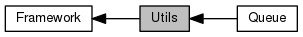
\includegraphics[width=218pt]{d6/dae/group___utils}
\end{center}
\end{figure}
\subsection*{Macros}
\begin{DoxyCompactItemize}
\item 
\#define \hyperlink{group___utils_ga0d57378e32bf8278011460740bc29f7f}{U\+A\+R\+T\+\_\+\+B\+U\+F\+F\+E\+R\+\_\+\+S\+I\+ZE}~4
\item 
\#define \hyperlink{group___utils_ga2345ec0af8fc8a1782768a22a15a4ad3}{D\+M\+A\+\_\+\+R\+X\+\_\+\+B\+U\+F\+F\+E\+R\+\_\+\+S\+I\+ZE}~4
\end{DoxyCompactItemize}
\subsection*{Enumerations}
\begin{DoxyCompactItemize}
\item 
enum \hyperlink{group___utils_gaf6a258d8f3ee5206d682d799316314b1}{bool} \{ \hyperlink{group___utils_ggaf6a258d8f3ee5206d682d799316314b1ae9de385ef6fe9bf3360d1038396b884c}{false} = 0, 
\hyperlink{group___utils_ggaf6a258d8f3ee5206d682d799316314b1a08f175a5505a10b9ed657defeb050e4b}{true} = !false
 \}
\end{DoxyCompactItemize}
\subsection*{Functions}
\begin{DoxyCompactItemize}
\item 
uint32\+\_\+t \hyperlink{group___utils_gafa33c555a40e71b0cc32aa3731f6fabe}{max} (uint32\+\_\+t a, uint32\+\_\+t b, uint32\+\_\+t c)
\begin{DoxyCompactList}\small\item\em Find max between a, b, and c. \end{DoxyCompactList}\item 
void \hyperlink{group___utils_gaf1a8629740f19d111a55636a19c2bf08}{delay} (uint32\+\_\+t microseconds)
\begin{DoxyCompactList}\small\item\em delay for the number of microsecond \end{DoxyCompactList}\end{DoxyCompactItemize}
\subsection*{Variables}
\begin{DoxyCompactItemize}
\item 
uint8\+\_\+t \hyperlink{group___utils_ga91a0f4b54880f52e0b02f7aeb96ca304}{pixel\+\_\+color}
\item 
uint8\+\_\+t \hyperlink{group___utils_gaead30033cf45bc8bbfab301a6c770afb}{D\+M\+A\+\_\+\+R\+X\+\_\+\+Buffer} \mbox{[}\hyperlink{group___utils_ga2345ec0af8fc8a1782768a22a15a4ad3}{D\+M\+A\+\_\+\+R\+X\+\_\+\+B\+U\+F\+F\+E\+R\+\_\+\+S\+I\+ZE}\mbox{]}
\item 
uint8\+\_\+t \hyperlink{group___utils_gab42d904ed5954df151e40839a2351427}{U\+A\+R\+T\+\_\+\+Buffer} \mbox{[}\hyperlink{group___utils_ga0d57378e32bf8278011460740bc29f7f}{U\+A\+R\+T\+\_\+\+B\+U\+F\+F\+E\+R\+\_\+\+S\+I\+ZE}\mbox{]}
\item 
uint8\+\_\+t \hyperlink{group___utils_ga91a0f4b54880f52e0b02f7aeb96ca304}{pixel\+\_\+color}
\item 
uint8\+\_\+t \hyperlink{group___utils_gaead30033cf45bc8bbfab301a6c770afb}{D\+M\+A\+\_\+\+R\+X\+\_\+\+Buffer} \mbox{[}\hyperlink{group___utils_ga2345ec0af8fc8a1782768a22a15a4ad3}{D\+M\+A\+\_\+\+R\+X\+\_\+\+B\+U\+F\+F\+E\+R\+\_\+\+S\+I\+ZE}\mbox{]}
\item 
uint8\+\_\+t \hyperlink{group___utils_gab42d904ed5954df151e40839a2351427}{U\+A\+R\+T\+\_\+\+Buffer} \mbox{[}\hyperlink{group___utils_ga0d57378e32bf8278011460740bc29f7f}{U\+A\+R\+T\+\_\+\+B\+U\+F\+F\+E\+R\+\_\+\+S\+I\+ZE}\mbox{]} = \{0\}
\end{DoxyCompactItemize}


\subsection{Detailed Description}
utils driver modules 



\subsection{Macro Definition Documentation}
\index{Utils@{Utils}!D\+M\+A\+\_\+\+R\+X\+\_\+\+B\+U\+F\+F\+E\+R\+\_\+\+S\+I\+ZE@{D\+M\+A\+\_\+\+R\+X\+\_\+\+B\+U\+F\+F\+E\+R\+\_\+\+S\+I\+ZE}}
\index{D\+M\+A\+\_\+\+R\+X\+\_\+\+B\+U\+F\+F\+E\+R\+\_\+\+S\+I\+ZE@{D\+M\+A\+\_\+\+R\+X\+\_\+\+B\+U\+F\+F\+E\+R\+\_\+\+S\+I\+ZE}!Utils@{Utils}}
\subsubsection[{\texorpdfstring{D\+M\+A\+\_\+\+R\+X\+\_\+\+B\+U\+F\+F\+E\+R\+\_\+\+S\+I\+ZE}{DMA_RX_BUFFER_SIZE}}]{\setlength{\rightskip}{0pt plus 5cm}\#define D\+M\+A\+\_\+\+R\+X\+\_\+\+B\+U\+F\+F\+E\+R\+\_\+\+S\+I\+ZE~4}\hypertarget{group___utils_ga2345ec0af8fc8a1782768a22a15a4ad3}{}\label{group___utils_ga2345ec0af8fc8a1782768a22a15a4ad3}


Definition at line 44 of file N\+P\+C\+\_\+utils.\+h.

\index{Utils@{Utils}!U\+A\+R\+T\+\_\+\+B\+U\+F\+F\+E\+R\+\_\+\+S\+I\+ZE@{U\+A\+R\+T\+\_\+\+B\+U\+F\+F\+E\+R\+\_\+\+S\+I\+ZE}}
\index{U\+A\+R\+T\+\_\+\+B\+U\+F\+F\+E\+R\+\_\+\+S\+I\+ZE@{U\+A\+R\+T\+\_\+\+B\+U\+F\+F\+E\+R\+\_\+\+S\+I\+ZE}!Utils@{Utils}}
\subsubsection[{\texorpdfstring{U\+A\+R\+T\+\_\+\+B\+U\+F\+F\+E\+R\+\_\+\+S\+I\+ZE}{UART_BUFFER_SIZE}}]{\setlength{\rightskip}{0pt plus 5cm}\#define U\+A\+R\+T\+\_\+\+B\+U\+F\+F\+E\+R\+\_\+\+S\+I\+ZE~4}\hypertarget{group___utils_ga0d57378e32bf8278011460740bc29f7f}{}\label{group___utils_ga0d57378e32bf8278011460740bc29f7f}


Definition at line 43 of file N\+P\+C\+\_\+utils.\+h.



\subsection{Enumeration Type Documentation}
\index{Utils@{Utils}!bool@{bool}}
\index{bool@{bool}!Utils@{Utils}}
\subsubsection[{\texorpdfstring{bool}{bool}}]{\setlength{\rightskip}{0pt plus 5cm}enum {\bf bool}}\hypertarget{group___utils_gaf6a258d8f3ee5206d682d799316314b1}{}\label{group___utils_gaf6a258d8f3ee5206d682d799316314b1}
\begin{Desc}
\item[Enumerator]\par
\begin{description}
\index{false@{false}!Utils@{Utils}}\index{Utils@{Utils}!false@{false}}\item[{\em 
false\hypertarget{group___utils_ggaf6a258d8f3ee5206d682d799316314b1ae9de385ef6fe9bf3360d1038396b884c}{}\label{group___utils_ggaf6a258d8f3ee5206d682d799316314b1ae9de385ef6fe9bf3360d1038396b884c}
}]\index{true@{true}!Utils@{Utils}}\index{Utils@{Utils}!true@{true}}\item[{\em 
true\hypertarget{group___utils_ggaf6a258d8f3ee5206d682d799316314b1a08f175a5505a10b9ed657defeb050e4b}{}\label{group___utils_ggaf6a258d8f3ee5206d682d799316314b1a08f175a5505a10b9ed657defeb050e4b}
}]\end{description}
\end{Desc}


Definition at line 40 of file N\+P\+C\+\_\+utils.\+h.



\subsection{Function Documentation}
\index{Utils@{Utils}!delay@{delay}}
\index{delay@{delay}!Utils@{Utils}}
\subsubsection[{\texorpdfstring{delay(uint32\+\_\+t microseconds)}{delay(uint32_t microseconds)}}]{\setlength{\rightskip}{0pt plus 5cm}void delay (
\begin{DoxyParamCaption}
\item[{uint32\+\_\+t}]{microseconds}
\end{DoxyParamCaption}
)}\hypertarget{group___utils_gaf1a8629740f19d111a55636a19c2bf08}{}\label{group___utils_gaf1a8629740f19d111a55636a19c2bf08}


delay for the number of microsecond 

\begin{DoxyNote}{Note}
T\+O\+DO use R\+T\+OS delay instead 
\end{DoxyNote}

\begin{DoxyParams}{Parameters}
{\em microseconds} & \\
\hline
\end{DoxyParams}

\begin{DoxyRetVals}{Return values}
{\em None} & \\
\hline
\end{DoxyRetVals}


Definition at line 59 of file N\+P\+C\+\_\+utils.\+c.



Here is the caller graph for this function\+:
\nopagebreak
\begin{figure}[H]
\begin{center}
\leavevmode
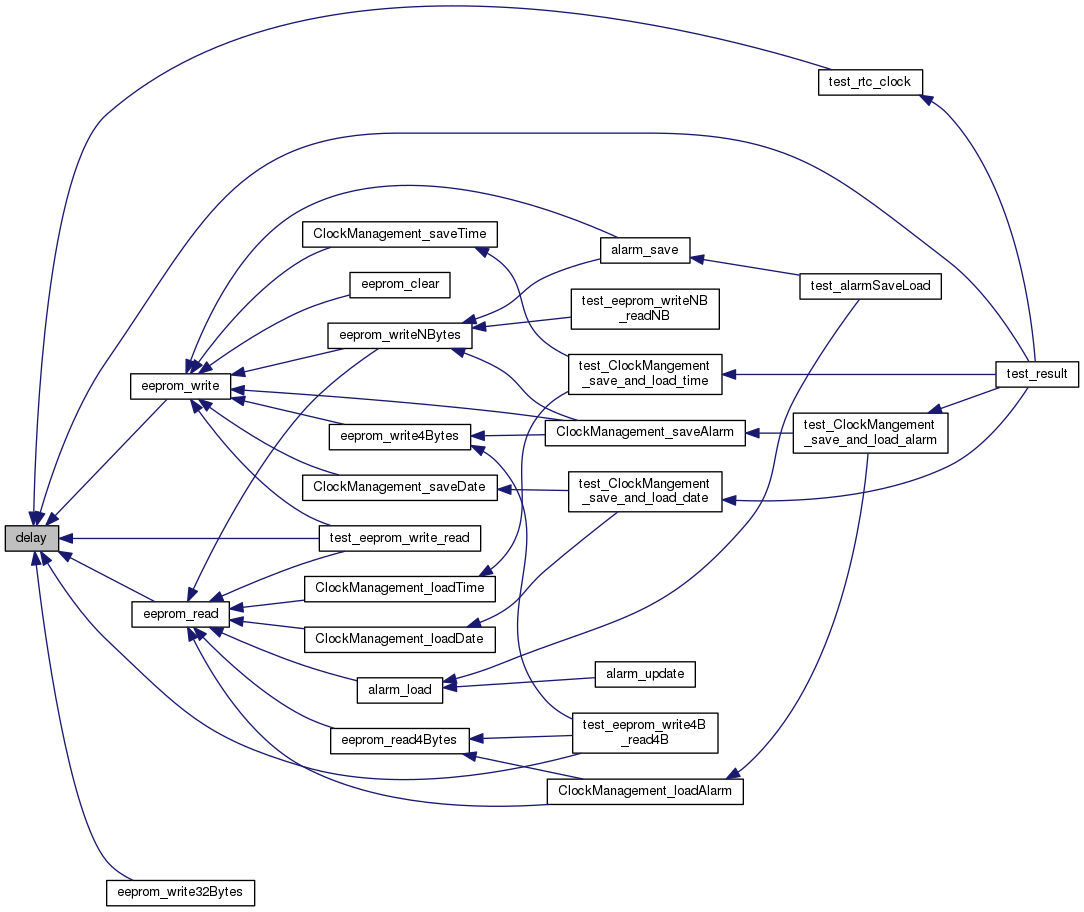
\includegraphics[width=350pt]{d6/dae/group___utils_gaf1a8629740f19d111a55636a19c2bf08_icgraph}
\end{center}
\end{figure}


\index{Utils@{Utils}!max@{max}}
\index{max@{max}!Utils@{Utils}}
\subsubsection[{\texorpdfstring{max(uint32\+\_\+t a, uint32\+\_\+t b, uint32\+\_\+t c)}{max(uint32_t a, uint32_t b, uint32_t c)}}]{\setlength{\rightskip}{0pt plus 5cm}uint32\+\_\+t max (
\begin{DoxyParamCaption}
\item[{uint32\+\_\+t}]{a, }
\item[{uint32\+\_\+t}]{b, }
\item[{uint32\+\_\+t}]{c}
\end{DoxyParamCaption}
)}\hypertarget{group___utils_gafa33c555a40e71b0cc32aa3731f6fabe}{}\label{group___utils_gafa33c555a40e71b0cc32aa3731f6fabe}


Find max between a, b, and c. 


\begin{DoxyParams}{Parameters}
{\em a} & First value \\
\hline
{\em b} & second value \\
\hline
{\em c} & Third value \\
\hline
\end{DoxyParams}

\begin{DoxyRetVals}{Return values}
{\em uint32\+\_\+t} & of the maximum value \\
\hline
\end{DoxyRetVals}


Definition at line 49 of file N\+P\+C\+\_\+utils.\+c.



Here is the caller graph for this function\+:\nopagebreak
\begin{figure}[H]
\begin{center}
\leavevmode
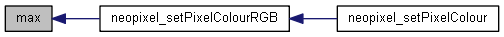
\includegraphics[width=350pt]{d6/dae/group___utils_gafa33c555a40e71b0cc32aa3731f6fabe_icgraph}
\end{center}
\end{figure}




\subsection{Variable Documentation}
\index{Utils@{Utils}!D\+M\+A\+\_\+\+R\+X\+\_\+\+Buffer@{D\+M\+A\+\_\+\+R\+X\+\_\+\+Buffer}}
\index{D\+M\+A\+\_\+\+R\+X\+\_\+\+Buffer@{D\+M\+A\+\_\+\+R\+X\+\_\+\+Buffer}!Utils@{Utils}}
\subsubsection[{\texorpdfstring{D\+M\+A\+\_\+\+R\+X\+\_\+\+Buffer}{DMA_RX_Buffer}}]{\setlength{\rightskip}{0pt plus 5cm}uint8\+\_\+t D\+M\+A\+\_\+\+R\+X\+\_\+\+Buffer\mbox{[}{\bf D\+M\+A\+\_\+\+R\+X\+\_\+\+B\+U\+F\+F\+E\+R\+\_\+\+S\+I\+ZE}\mbox{]}}\hypertarget{group___utils_gaead30033cf45bc8bbfab301a6c770afb}{}\label{group___utils_gaead30033cf45bc8bbfab301a6c770afb}


Definition at line 38 of file N\+P\+C\+\_\+utils.\+c.

\index{Utils@{Utils}!D\+M\+A\+\_\+\+R\+X\+\_\+\+Buffer@{D\+M\+A\+\_\+\+R\+X\+\_\+\+Buffer}}
\index{D\+M\+A\+\_\+\+R\+X\+\_\+\+Buffer@{D\+M\+A\+\_\+\+R\+X\+\_\+\+Buffer}!Utils@{Utils}}
\subsubsection[{\texorpdfstring{D\+M\+A\+\_\+\+R\+X\+\_\+\+Buffer}{DMA_RX_Buffer}}]{\setlength{\rightskip}{0pt plus 5cm}uint8\+\_\+t D\+M\+A\+\_\+\+R\+X\+\_\+\+Buffer\mbox{[}{\bf D\+M\+A\+\_\+\+R\+X\+\_\+\+B\+U\+F\+F\+E\+R\+\_\+\+S\+I\+ZE}\mbox{]}}\hypertarget{group___utils_gaead30033cf45bc8bbfab301a6c770afb}{}\label{group___utils_gaead30033cf45bc8bbfab301a6c770afb}


Definition at line 38 of file N\+P\+C\+\_\+utils.\+c.

\index{Utils@{Utils}!pixel\+\_\+color@{pixel\+\_\+color}}
\index{pixel\+\_\+color@{pixel\+\_\+color}!Utils@{Utils}}
\subsubsection[{\texorpdfstring{pixel\+\_\+color}{pixel_color}}]{\setlength{\rightskip}{0pt plus 5cm}uint8\+\_\+t pixel\+\_\+color}\hypertarget{group___utils_ga91a0f4b54880f52e0b02f7aeb96ca304}{}\label{group___utils_ga91a0f4b54880f52e0b02f7aeb96ca304}


Definition at line 36 of file N\+P\+C\+\_\+utils.\+c.

\index{Utils@{Utils}!pixel\+\_\+color@{pixel\+\_\+color}}
\index{pixel\+\_\+color@{pixel\+\_\+color}!Utils@{Utils}}
\subsubsection[{\texorpdfstring{pixel\+\_\+color}{pixel_color}}]{\setlength{\rightskip}{0pt plus 5cm}uint8\+\_\+t pixel\+\_\+color}\hypertarget{group___utils_ga91a0f4b54880f52e0b02f7aeb96ca304}{}\label{group___utils_ga91a0f4b54880f52e0b02f7aeb96ca304}


Definition at line 36 of file N\+P\+C\+\_\+utils.\+c.

\index{Utils@{Utils}!U\+A\+R\+T\+\_\+\+Buffer@{U\+A\+R\+T\+\_\+\+Buffer}}
\index{U\+A\+R\+T\+\_\+\+Buffer@{U\+A\+R\+T\+\_\+\+Buffer}!Utils@{Utils}}
\subsubsection[{\texorpdfstring{U\+A\+R\+T\+\_\+\+Buffer}{UART_Buffer}}]{\setlength{\rightskip}{0pt plus 5cm}uint8\+\_\+t U\+A\+R\+T\+\_\+\+Buffer\mbox{[}{\bf U\+A\+R\+T\+\_\+\+B\+U\+F\+F\+E\+R\+\_\+\+S\+I\+ZE}\mbox{]} = \{0\}}\hypertarget{group___utils_gab42d904ed5954df151e40839a2351427}{}\label{group___utils_gab42d904ed5954df151e40839a2351427}


Definition at line 39 of file N\+P\+C\+\_\+utils.\+c.

\index{Utils@{Utils}!U\+A\+R\+T\+\_\+\+Buffer@{U\+A\+R\+T\+\_\+\+Buffer}}
\index{U\+A\+R\+T\+\_\+\+Buffer@{U\+A\+R\+T\+\_\+\+Buffer}!Utils@{Utils}}
\subsubsection[{\texorpdfstring{U\+A\+R\+T\+\_\+\+Buffer}{UART_Buffer}}]{\setlength{\rightskip}{0pt plus 5cm}uint8\+\_\+t U\+A\+R\+T\+\_\+\+Buffer\mbox{[}{\bf U\+A\+R\+T\+\_\+\+B\+U\+F\+F\+E\+R\+\_\+\+S\+I\+ZE}\mbox{]}}\hypertarget{group___utils_gab42d904ed5954df151e40839a2351427}{}\label{group___utils_gab42d904ed5954df151e40839a2351427}


Definition at line 39 of file N\+P\+C\+\_\+utils.\+c.


\hypertarget{group___n_p_c}{}\section{N\+PC}
\label{group___n_p_c}\index{N\+PC@{N\+PC}}
\subsection*{Modules}
\begin{DoxyCompactItemize}
\item 
\hyperlink{group___audio}{Audio}
\begin{DoxyCompactList}\small\item\em Manage audio configuration and play audio. \end{DoxyCompactList}\item 
\hyperlink{group___bluetooth}{Bluetooth}
\begin{DoxyCompactList}\small\item\em Bluetooth driver modules. \end{DoxyCompactList}\item 
\hyperlink{group___clock}{Clock}
\begin{DoxyCompactList}\small\item\em Clock driver modules. \end{DoxyCompactList}\item 
\hyperlink{group___configuration}{Configuration}
\begin{DoxyCompactList}\small\item\em Configuration driver modules. \end{DoxyCompactList}\item 
\hyperlink{group___eeprom}{Eeprom}
\begin{DoxyCompactList}\small\item\em Eeprom framework. \end{DoxyCompactList}\item 
\hyperlink{group___neo_pixel}{Neo\+Pixel}
\begin{DoxyCompactList}\small\item\em neopixel driver modules \end{DoxyCompactList}\item 
\hyperlink{group___temperature}{Temperature}
\item 
\hyperlink{group___utils}{Utils}
\begin{DoxyCompactList}\small\item\em utils driver modules \end{DoxyCompactList}\end{DoxyCompactItemize}


\subsection{Detailed Description}

\chapter{File Documentation}
\hypertarget{_n_p_c__audio_8h}{}\section{C\+:/\+Users/\+Kojey/\+Desktop/\+N\+P\+C/\+Neo\+Pixel\+Clock\+\_\+\+Software/\+Code/\+Libraries/\+N\+P\+C/inc/\+N\+P\+C\+\_\+audio.h File Reference}
\label{_n_p_c__audio_8h}\index{C\+:/\+Users/\+Kojey/\+Desktop/\+N\+P\+C/\+Neo\+Pixel\+Clock\+\_\+\+Software/\+Code/\+Libraries/\+N\+P\+C/inc/\+N\+P\+C\+\_\+audio.\+h@{C\+:/\+Users/\+Kojey/\+Desktop/\+N\+P\+C/\+Neo\+Pixel\+Clock\+\_\+\+Software/\+Code/\+Libraries/\+N\+P\+C/inc/\+N\+P\+C\+\_\+audio.\+h}}


This file contains all the configuration prototypes used by the audio firmware.  


{\ttfamily \#include \char`\"{}N\+P\+C\+\_\+utils.\+h\char`\"{}}\newline
\subsection*{Macros}
\begin{DoxyCompactItemize}
\item 
\#define {\bfseries A\+U\+D\+I\+O\+\_\+\+F\+R\+E\+Q\+U\+E\+N\+CY}~11000
\item 
\#define {\bfseries D\+M\+A\+\_\+\+F\+R\+E\+Q\+U\+E\+N\+CY}~(86000000/(2$\ast$A\+U\+D\+I\+O\+\_\+\+F\+R\+E\+Q\+U\+E\+N\+CY))
\end{DoxyCompactItemize}
\subsection*{Functions}
\begin{DoxyCompactItemize}
\item 
void \hyperlink{group___audio_gafff6cd7f4332d078ce0114143cd30998}{audio\+\_\+disable} (void)
\begin{DoxyCompactList}\small\item\em Disable the D\+MA. \end{DoxyCompactList}\item 
void \hyperlink{group___audio_ga6a621a84280fa05373990982dacce11b}{audio\+\_\+init} (uint16\+\_\+t $\ast$, uint16\+\_\+t)
\begin{DoxyCompactList}\small\item\em Perform audio initialization. \end{DoxyCompactList}\item 
void \hyperlink{group___audio_ga286b07d3729ae2bfdf88bcd777dd93cf}{audio\+\_\+play} (uint16\+\_\+t $\ast$, uint16\+\_\+t)
\begin{DoxyCompactList}\small\item\em Play a sample. \end{DoxyCompactList}\end{DoxyCompactItemize}


\subsection{Detailed Description}
This file contains all the configuration prototypes used by the audio firmware. 

\begin{DoxyAuthor}{Author}
Othniel Konan (Kojey) 
\end{DoxyAuthor}
\begin{DoxyVersion}{Version}
V1.\+1.\+0 
\end{DoxyVersion}
\begin{DoxyDate}{Date}
12-\/\+March-\/2017 
\end{DoxyDate}
\begin{DoxyAttention}{Attention}

\end{DoxyAttention}
\subsubsection*{\begin{center}\copyright{} C\+O\+P\+Y\+R\+I\+G\+HT \end{center} }
\hypertarget{_n_p_c__bluetooth_8h}{}\section{N\+P\+C\+\_\+bluetooth.\+h File Reference}
\label{_n_p_c__bluetooth_8h}\index{N\+P\+C\+\_\+bluetooth.\+h@{N\+P\+C\+\_\+bluetooth.\+h}}


This file contains all the configuration prototypes used by the bluetooth firmware.  


{\ttfamily \#include \char`\"{}N\+P\+C\+\_\+utils.\+h\char`\"{}}\\*
Include dependency graph for N\+P\+C\+\_\+bluetooth.\+h\+:
\nopagebreak
\begin{figure}[H]
\begin{center}
\leavevmode
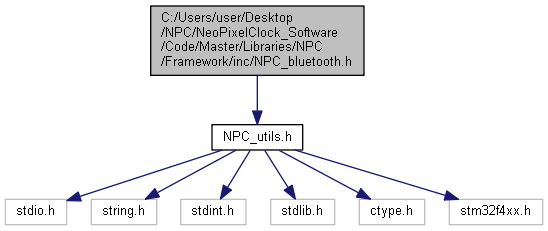
\includegraphics[width=350pt]{d8/d27/_n_p_c__bluetooth_8h__incl}
\end{center}
\end{figure}
This graph shows which files directly or indirectly include this file\+:
\nopagebreak
\begin{figure}[H]
\begin{center}
\leavevmode
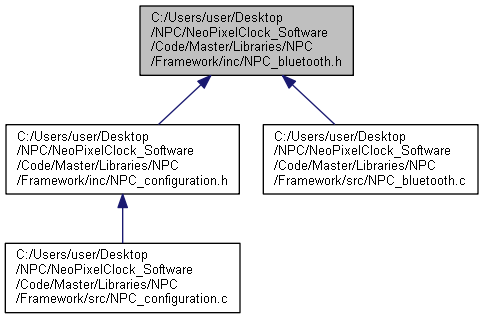
\includegraphics[width=298pt]{df/dc7/_n_p_c__bluetooth_8h__dep__incl}
\end{center}
\end{figure}
\subsection*{Macros}
\begin{DoxyCompactItemize}
\item 
\#define \hyperlink{group__bluetooth___constants_gac4b97204cfdd1ad5faebd0a56a6521c6}{B\+L\+U\+E\+T\+O\+O\+T\+H\+\_\+\+P\+E\+R\+I\+P\+H\+\_\+\+U\+S\+A\+R\+TX}~R\+C\+C\+\_\+\+A\+P\+B2\+Periph\+\_\+\+U\+S\+A\+R\+T1
\item 
\#define \hyperlink{group__bluetooth___constants_gab9bf1b33e271246e795a3847516e0949}{B\+L\+U\+E\+T\+O\+O\+T\+H\+\_\+\+P\+E\+R\+I\+P\+H\+\_\+\+G\+P\+I\+OX}~R\+C\+C\+\_\+\+A\+H\+B1\+Periph\+\_\+\+G\+P\+I\+OB
\item 
\#define \hyperlink{group__bluetooth___constants_gad47fcf58a7d55e48e039420b36350fcd}{B\+L\+U\+E\+T\+O\+O\+T\+H\+\_\+\+G\+P\+I\+OX}~G\+P\+I\+OB
\item 
\#define \hyperlink{group__bluetooth___constants_ga03828dc38b1dd4e24867280ccaf54c1e}{B\+L\+U\+E\+T\+O\+O\+T\+H\+\_\+\+T\+X\+\_\+\+P\+IN}~G\+P\+I\+O\+\_\+\+Pin\+\_\+6
\item 
\#define \hyperlink{group__bluetooth___constants_gad6b845bce7449baa7ebc4f2625c32165}{B\+L\+U\+E\+T\+O\+O\+T\+H\+\_\+\+R\+X\+\_\+\+P\+IN}~G\+P\+I\+O\+\_\+\+Pin\+\_\+7
\item 
\#define \hyperlink{group__bluetooth___constants_gaae23de9ae44f36e0a519e010e545d579}{B\+L\+U\+E\+T\+O\+O\+T\+H\+\_\+\+T\+X\+\_\+\+P\+I\+N\+S\+O\+U\+R\+CE}~G\+P\+I\+O\+\_\+\+Pin\+Source6
\item 
\#define \hyperlink{group__bluetooth___constants_gaf8abe33a7c3b953bc50789da61176ce8}{B\+L\+U\+E\+T\+O\+O\+T\+H\+\_\+\+R\+X\+\_\+\+P\+I\+N\+S\+O\+U\+R\+CE}~G\+P\+I\+O\+\_\+\+Pin\+Source7
\item 
\#define \hyperlink{group__bluetooth___constants_ga89cad714e99e26757fe9208e98c6cbe9}{B\+L\+U\+E\+T\+O\+O\+T\+H\+\_\+\+A\+F\+\_\+\+U\+S\+A\+RT}~G\+P\+I\+O\+\_\+\+A\+F\+\_\+\+U\+S\+A\+R\+T1
\item 
\#define \hyperlink{group__bluetooth___constants_gac9aff5be09be7a2e3c84d99794f80dc3}{B\+L\+U\+E\+T\+O\+O\+T\+H\+\_\+\+U\+S\+A\+R\+TX}~U\+S\+A\+R\+T1
\item 
\#define \hyperlink{group__bluetooth___constants_ga6049290b6a001e8af7bc24ebe06f8ee8}{B\+L\+U\+E\+T\+O\+O\+T\+H\+\_\+\+U\+S\+A\+R\+T\+X\+\_\+\+I\+RQ}~U\+S\+A\+R\+T1\+\_\+\+I\+R\+Qn
\item 
\#define \hyperlink{group__bluetooth___constants_ga800ec9bb77245339c6a2b770432e0232}{B\+L\+U\+E\+T\+O\+O\+T\+H\+\_\+\+B\+A\+U\+D\+R\+A\+TE}~9600
\end{DoxyCompactItemize}
\subsection*{Functions}
\begin{DoxyCompactItemize}
\item 
void \hyperlink{group__bluetooth___init_gaaa60810e0857e9e1e5b2cba80b8db3ff}{bluetooth\+\_\+init} (void)
\begin{DoxyCompactList}\small\item\em Initialize the bluetooth and set baudrate to 9600. \end{DoxyCompactList}\item 
void \hyperlink{group__bluetooth___init_ga7139cd4baabbbcbab0c1fe6d7d4ae1cc}{U\+S\+A\+R\+T1\+\_\+\+I\+R\+Q\+Handler} (void)
\begin{DoxyCompactList}\small\item\em Global interrupt handler for U\+S\+A\+R\+T1. \end{DoxyCompactList}\item 
void \hyperlink{group__bluetooth___init_gaef190d87febc0414eb7a39bd4c2d2169}{D\+M\+A2\+\_\+\+Stream5\+\_\+\+I\+R\+Q\+Handler} (void)
\begin{DoxyCompactList}\small\item\em Global interrupt handler for D\+M\+A2 stream5. \end{DoxyCompactList}\item 
void \hyperlink{group__bluetooth___trans_ga31d829d5658369ee2c90b9c3cdbedfe1}{bluetooth\+\_\+send} (uint8\+\_\+t $\ast$data)
\begin{DoxyCompactList}\small\item\em send string to the hc-\/06 \end{DoxyCompactList}\end{DoxyCompactItemize}
\subsection*{Variables}
\begin{DoxyCompactItemize}
\item 
size\+\_\+t \hyperlink{group__bluetooth_ga7143c37ba48173d0e245161e9ddc3592}{bluetooth\+\_\+write}
\item 
size\+\_\+t \hyperlink{group__bluetooth_ga723054cd6b30ca246f123b25e099146d}{bluetooth\+\_\+read}
\end{DoxyCompactItemize}


\subsection{Detailed Description}
This file contains all the configuration prototypes used by the bluetooth firmware. 

\begin{DoxyAuthor}{Author}
Othniel Konan (Kojey) 
\end{DoxyAuthor}
\begin{DoxyVersion}{Version}
V1.\+1.\+0 
\end{DoxyVersion}
\begin{DoxyDate}{Date}
01-\/\+March-\/2017 
\end{DoxyDate}
\begin{DoxyAttention}{Attention}

\end{DoxyAttention}
\subsubsection*{\begin{center}\copyright{} C\+O\+P\+Y\+R\+I\+G\+HT \end{center} }
\hypertarget{_n_p_c__clock_8h}{}\section{C\+:/\+Users/\+Kojey/\+Desktop/\+N\+P\+C/\+Neo\+Pixel\+Clock\+\_\+\+Software/\+Code/\+Libraries/\+N\+P\+C/\+Framework/inc/\+N\+P\+C\+\_\+clock.h File Reference}
\label{_n_p_c__clock_8h}\index{C\+:/\+Users/\+Kojey/\+Desktop/\+N\+P\+C/\+Neo\+Pixel\+Clock\+\_\+\+Software/\+Code/\+Libraries/\+N\+P\+C/\+Framework/inc/\+N\+P\+C\+\_\+clock.\+h@{C\+:/\+Users/\+Kojey/\+Desktop/\+N\+P\+C/\+Neo\+Pixel\+Clock\+\_\+\+Software/\+Code/\+Libraries/\+N\+P\+C/\+Framework/inc/\+N\+P\+C\+\_\+clock.\+h}}


This file contains all the functions prototypes for the clock firmware library used for the N\+PC.  


{\ttfamily \#include \char`\"{}N\+P\+C\+\_\+utils.\+h\char`\"{}}\newline
Include dependency graph for N\+P\+C\+\_\+clock.\+h\+:
% FIG 0
This graph shows which files directly or indirectly include this file\+:
% FIG 1
\subsection*{Macros}
\begin{DoxyCompactItemize}
\item 
\#define {\bfseries R\+T\+C\+\_\+\+P\+R\+E\+D\+I\+V\+\_\+A}~0x7C
\item 
\#define {\bfseries R\+T\+C\+\_\+\+P\+R\+E\+D\+I\+V\+\_\+S}~0\+X1\+F3F
\item 
\#define {\bfseries C\+L\+O\+C\+K\+\_\+A}~R\+T\+C\+\_\+\+Alarm\+\_\+A
\item 
\#define {\bfseries C\+L\+O\+C\+K\+\_\+B}~R\+T\+C\+\_\+\+Alarm\+\_\+B
\item 
\#define {\bfseries C\+L\+O\+C\+K\+\_\+\+AM}~R\+T\+C\+\_\+\+H12\+\_\+\+AM
\item 
\#define {\bfseries C\+L\+O\+C\+K\+\_\+\+PM}~R\+T\+C\+\_\+\+H12\+\_\+\+PM
\item 
\#define {\bfseries C\+L\+O\+C\+K\+\_\+\+Week\+Day}~(uint8\+\_\+t) (\hyperlink{group___clock___time___date_gabb4d72928cb3d131d40067fb141003aa}{clock\+\_\+get\+Date}() $>$$>$ 24)
\item 
\#define {\bfseries C\+L\+O\+C\+K\+\_\+\+Month}~(uint8\+\_\+t) (\hyperlink{group___clock___time___date_gabb4d72928cb3d131d40067fb141003aa}{clock\+\_\+get\+Date}() $>$$>$ 16)
\item 
\#define {\bfseries C\+L\+O\+C\+K\+\_\+date}~(uint8\+\_\+t) (\hyperlink{group___clock___time___date_gabb4d72928cb3d131d40067fb141003aa}{clock\+\_\+get\+Date}() $>$$>$ 8)
\item 
\#define {\bfseries C\+L\+O\+C\+K\+\_\+\+Year}~(uint8\+\_\+t) \hyperlink{group___clock___time___date_gabb4d72928cb3d131d40067fb141003aa}{clock\+\_\+get\+Date}()
\item 
\#define {\bfseries C\+L\+O\+C\+K\+\_\+\+Hours}~(uint8\+\_\+t) (\hyperlink{group___clock___time___date_ga03ae6948083c259f6edc0b146f40dc62}{clock\+\_\+get\+Time}() $>$$>$ 24)
\item 
\#define {\bfseries C\+L\+O\+C\+K\+\_\+\+Minutes}~(uint8\+\_\+t) (\hyperlink{group___clock___time___date_ga03ae6948083c259f6edc0b146f40dc62}{clock\+\_\+get\+Time}() $>$$>$ 16)
\item 
\#define {\bfseries C\+L\+O\+C\+K\+\_\+seconds}~(uint8\+\_\+t) (\hyperlink{group___clock___time___date_ga03ae6948083c259f6edc0b146f40dc62}{clock\+\_\+get\+Time}() $>$$>$ 8)
\item 
\#define {\bfseries C\+L\+O\+C\+K\+\_\+\+Format}~(uint8\+\_\+t) \hyperlink{group___clock___time___date_ga03ae6948083c259f6edc0b146f40dc62}{clock\+\_\+get\+Time}()
\item 
\#define {\bfseries R\+E\+P\+E\+A\+T\+\_\+\+Date\+Week\+Day}~(uint32\+\_\+t) R\+T\+C\+\_\+\+Alarm\+Mask\+\_\+\+Date\+Week\+Day
\item 
\#define {\bfseries R\+E\+P\+E\+A\+T\+\_\+\+Hours}~(uint32\+\_\+t) R\+T\+C\+\_\+\+Alarm\+Mask\+\_\+\+Hours
\item 
\#define {\bfseries R\+E\+P\+E\+A\+T\+\_\+\+Minutes}~(uint32\+\_\+t) R\+T\+C\+\_\+\+Alarm\+Mask\+\_\+\+Minutes
\item 
\#define {\bfseries R\+E\+P\+E\+A\+T\+\_\+\+Seconds}~(uint32\+\_\+t) R\+T\+C\+\_\+\+Alarm\+Mask\+\_\+\+Seconds
\item 
\#define {\bfseries R\+E\+P\+E\+A\+T\+\_\+\+None}~(uint32\+\_\+t) R\+T\+C\+\_\+\+Alarm\+Mask\+\_\+\+None
\end{DoxyCompactItemize}
\subsection*{Functions}
\begin{DoxyCompactItemize}
\item 
void \hyperlink{group___clock_ga78ab77b57cf2e00089f0a3a22508524c}{clock\+\_\+init} (void)
\begin{DoxyCompactList}\small\item\em Initialise the clock to 1\+Hz and setup peripherals for Alarm. \end{DoxyCompactList}\item 
Error\+Status \hyperlink{group___clock_gaf16498fa2702bfda6b89a3335ccc7ca6}{clock\+\_\+set\+Date} (uint8\+\_\+t week\+Day, uint8\+\_\+t month, uint8\+\_\+t date, uint8\+\_\+t year)
\begin{DoxyCompactList}\small\item\em Set the clock\textquotesingle{}s date. \end{DoxyCompactList}\item 
Error\+Status \hyperlink{group___clock_ga11404197d58ddf6b46230bcde4282ef2}{clock\+\_\+set\+Time} (uint8\+\_\+t am\+\_\+pm, uint8\+\_\+t hours, uint8\+\_\+t minutes, uint8\+\_\+t second)
\begin{DoxyCompactList}\small\item\em Set the clock\textquotesingle{}s time. \end{DoxyCompactList}\item 
uint32\+\_\+t \hyperlink{group___clock_gabb4d72928cb3d131d40067fb141003aa}{clock\+\_\+get\+Date} (void)
\begin{DoxyCompactList}\small\item\em Get the date encoded in a 32b format. \end{DoxyCompactList}\item 
uint32\+\_\+t \hyperlink{group___clock_ga03ae6948083c259f6edc0b146f40dc62}{clock\+\_\+get\+Time} (void)
\begin{DoxyCompactList}\small\item\em Get the time encoded in a 32b format. \end{DoxyCompactList}\item 
R\+T\+C\+\_\+\+Alarm\+Type\+Def \hyperlink{group___clock_ga5e1614dbb1a210106dbade3f133db27e}{clock\+\_\+create\+Alarm} (uint8\+\_\+t am\+\_\+pm, uint8\+\_\+t hours, uint8\+\_\+t minutes, uint8\+\_\+t seconds, uint32\+\_\+t date\+Week\+Day\+Sel, uint8\+\_\+t date\+Week\+Day, uint32\+\_\+t repeat)
\begin{DoxyCompactList}\small\item\em Create an Alarm Structure given all the parameters. \end{DoxyCompactList}\item 
void \hyperlink{group___clock_gab56f512746d4f2638232db28bb7dac2b}{clock\+\_\+setA} (R\+T\+C\+\_\+\+Alarm\+Type\+Def $\ast$Alarm)
\begin{DoxyCompactList}\small\item\em Set an alarm to R\+T\+C\+\_\+\+Alarm\+\_\+A, given a Alarm structure R\+T\+C\+\_\+\+Alarm\+Type\+Def. \end{DoxyCompactList}\item 
void \hyperlink{group___clock_gaea1a099c4ad6de8b99517ac6453e3569}{clock\+\_\+set\+Alarm} (uint8\+\_\+t am\+\_\+pm, uint8\+\_\+t hours, uint8\+\_\+t minutes, uint8\+\_\+t seconds, uint32\+\_\+t date\+Week\+Day\+Sel, uint8\+\_\+t date\+Week\+Day, uint32\+\_\+t repeat)
\begin{DoxyCompactList}\small\item\em Set an alarm to R\+T\+C\+\_\+\+Alarm\+\_\+A, given all the alarm parameters. \end{DoxyCompactList}\item 
void \hyperlink{group___clock_ga4da4fb52ec579671d337938e78f9a207}{R\+T\+C\+\_\+\+Alarm\+\_\+\+I\+R\+Q\+Handler} (void)
\begin{DoxyCompactList}\small\item\em Alarm Handler. \end{DoxyCompactList}\end{DoxyCompactItemize}


\subsection{Detailed Description}
This file contains all the functions prototypes for the clock firmware library used for the N\+PC. 

\begin{DoxyAuthor}{Author}
Othniel Konan (Kojey) 
\end{DoxyAuthor}
\begin{DoxyVersion}{Version}
V1.\+1.\+0 
\end{DoxyVersion}
\begin{DoxyDate}{Date}
06-\/\+March-\/2017 
\end{DoxyDate}
\begin{DoxyAttention}{Attention}

\end{DoxyAttention}
\subsubsection*{\begin{center}\copyright{} C\+O\+P\+Y\+R\+I\+G\+HT \end{center} }
\hypertarget{_n_p_c__configuration_8h}{}\section{N\+P\+C\+\_\+configuration.\+h File Reference}
\label{_n_p_c__configuration_8h}\index{N\+P\+C\+\_\+configuration.\+h@{N\+P\+C\+\_\+configuration.\+h}}


This file contains all the main initialization prototypes used by the N\+PC.  


{\ttfamily \#include \char`\"{}N\+P\+C\+\_\+bluetooth.\+h\char`\"{}}\\*
{\ttfamily \#include \char`\"{}N\+P\+C\+\_\+clock.\+h\char`\"{}}\\*
{\ttfamily \#include \char`\"{}N\+P\+C\+\_\+neopixel.\+h\char`\"{}}\\*
{\ttfamily \#include \char`\"{}N\+P\+C\+\_\+audio.\+h\char`\"{}}\\*
{\ttfamily \#include \char`\"{}N\+P\+C\+\_\+eeprom.\+h\char`\"{}}\\*
{\ttfamily \#include \char`\"{}N\+P\+C\+\_\+temperature.\+h\char`\"{}}\\*
Include dependency graph for N\+P\+C\+\_\+configuration.\+h\+:
\nopagebreak
\begin{figure}[H]
\begin{center}
\leavevmode
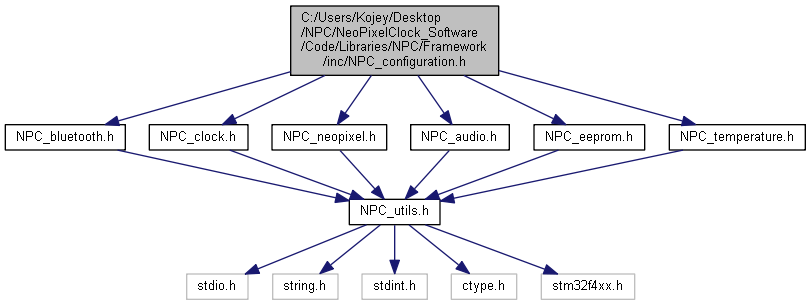
\includegraphics[width=350pt]{df/dfa/_n_p_c__configuration_8h__incl}
\end{center}
\end{figure}
This graph shows which files directly or indirectly include this file\+:
\nopagebreak
\begin{figure}[H]
\begin{center}
\leavevmode
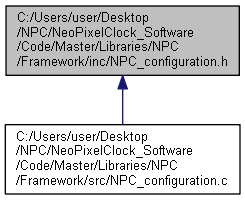
\includegraphics[width=187pt]{d8/d64/_n_p_c__configuration_8h__dep__incl}
\end{center}
\end{figure}
\subsection*{Functions}
\begin{DoxyCompactItemize}
\item 
void \hyperlink{group___configuration_gabe73c51b6f7ce590321d186bef079fe4}{N\+P\+C\+\_\+init} (void)
\begin{DoxyCompactList}\small\item\em Initialize all firmwares used by the N\+PC. \end{DoxyCompactList}\item 
void \hyperlink{group___configuration_ga1730ffe1e560465665eb47d9264826f9}{Error\+\_\+\+Handler} (void)
\begin{DoxyCompactList}\small\item\em This function is executed in case of error occurrence. \end{DoxyCompactList}\end{DoxyCompactItemize}


\subsection{Detailed Description}
This file contains all the main initialization prototypes used by the N\+PC. 

\begin{DoxyAuthor}{Author}
Othniel Konan (Kojey) 
\end{DoxyAuthor}
\begin{DoxyVersion}{Version}
V1.\+1.\+0 
\end{DoxyVersion}
\begin{DoxyDate}{Date}
17-\/\+February-\/2017 
\end{DoxyDate}
\begin{DoxyAttention}{Attention}

\end{DoxyAttention}
\subsubsection*{\begin{center}\copyright{} C\+O\+P\+Y\+R\+I\+G\+HT \end{center} }
\hypertarget{_n_p_c__eeprom_8h}{}\section{C\+:/\+Users/\+Kojey/\+Desktop/\+N\+P\+C/\+Neo\+Pixel\+Clock\+\_\+\+Software/\+Code/\+Libraries/\+N\+P\+C/inc/\+N\+P\+C\+\_\+eeprom.h File Reference}
\label{_n_p_c__eeprom_8h}\index{C\+:/\+Users/\+Kojey/\+Desktop/\+N\+P\+C/\+Neo\+Pixel\+Clock\+\_\+\+Software/\+Code/\+Libraries/\+N\+P\+C/inc/\+N\+P\+C\+\_\+eeprom.\+h@{C\+:/\+Users/\+Kojey/\+Desktop/\+N\+P\+C/\+Neo\+Pixel\+Clock\+\_\+\+Software/\+Code/\+Libraries/\+N\+P\+C/inc/\+N\+P\+C\+\_\+eeprom.\+h}}


This file contains all the configuration prototypes used by the eeprom firmware.  


{\ttfamily \#include \char`\"{}N\+P\+C\+\_\+utils.\+h\char`\"{}}\newline
\subsection*{Macros}
\begin{DoxyCompactItemize}
\item 
\#define {\bfseries W\+R\+EN}~0b00000110
\item 
\#define {\bfseries W\+R\+DI}~0b00000100
\item 
\#define {\bfseries R\+D\+SR}~0b00000101
\item 
\#define {\bfseries W\+R\+SR}~0b00000001
\item 
\#define {\bfseries R\+E\+AD}~0b00000011
\item 
\#define {\bfseries W\+R\+I\+TE}~0b00000010
\item 
\#define {\bfseries P\+A\+G\+E\+\_\+\+L\+E\+N\+G\+TH}~32
\end{DoxyCompactItemize}
\subsection*{Functions}
\begin{DoxyCompactItemize}
\item 
void \hyperlink{group___eeprom_ga4ec7f9d780da432051aa74ec5892a94c}{eeprom\+\_\+init} (void)
\begin{DoxyCompactList}\small\item\em Initialise communication to the eeprom. \end{DoxyCompactList}\item 
void \hyperlink{group___eeprom_ga11e27abf76759a5907ef18d1351aecdb}{eeprom\+\_\+write} (uint16\+\_\+t address, uint8\+\_\+t data)
\begin{DoxyCompactList}\small\item\em Write a byte to the eeprom. \end{DoxyCompactList}\item 
uint8\+\_\+t \hyperlink{group___eeprom_gafaa7cca6f6ad1d9ae49522324c825c2f}{eeprom\+\_\+read} (uint16\+\_\+t address)
\begin{DoxyCompactList}\small\item\em Read a byte from the eeprom. \end{DoxyCompactList}\item 
void \hyperlink{group___eeprom_ga4f1a1c3f7642565b9dbff6bfd2e7ed0d}{eeprom\+\_\+write32\+Bytes} (uint16\+\_\+t base\+Address, uint8\+\_\+t $\ast$data)
\begin{DoxyCompactList}\small\item\em Write a page to the eeprom. \end{DoxyCompactList}\item 
void \hyperlink{group___eeprom_ga7964a5a66da1c4a59a42309a93752217}{eeprom\+\_\+clear} (void)
\begin{DoxyCompactList}\small\item\em Clear eeprom data. \end{DoxyCompactList}\end{DoxyCompactItemize}


\subsection{Detailed Description}
This file contains all the configuration prototypes used by the eeprom firmware. 

\begin{DoxyAuthor}{Author}
Othniel Konan (Kojey) 
\end{DoxyAuthor}
\begin{DoxyVersion}{Version}
V1.\+1.\+0 
\end{DoxyVersion}
\begin{DoxyDate}{Date}
12-\/\+March-\/2017 
\end{DoxyDate}
\begin{DoxyAttention}{Attention}

\end{DoxyAttention}
\subsubsection*{\begin{center}\copyright{} C\+O\+P\+Y\+R\+I\+G\+HT \end{center} }
\hypertarget{_n_p_c__neopixel_8h}{}\section{N\+P\+C\+\_\+neopixel.\+h File Reference}
\label{_n_p_c__neopixel_8h}\index{N\+P\+C\+\_\+neopixel.\+h@{N\+P\+C\+\_\+neopixel.\+h}}


This file contains all the configuration prototypes used by the neopixel firmware.  


{\ttfamily \#include \char`\"{}N\+P\+C\+\_\+utils.\+h\char`\"{}}\\*
Include dependency graph for N\+P\+C\+\_\+neopixel.\+h\+:
\nopagebreak
\begin{figure}[H]
\begin{center}
\leavevmode
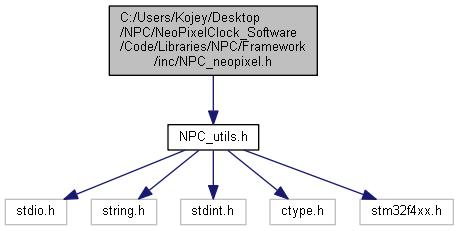
\includegraphics[width=350pt]{d5/db0/_n_p_c__neopixel_8h__incl}
\end{center}
\end{figure}
This graph shows which files directly or indirectly include this file\+:
\nopagebreak
\begin{figure}[H]
\begin{center}
\leavevmode
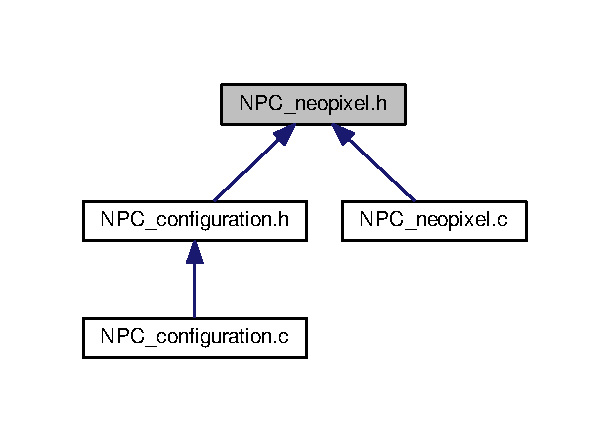
\includegraphics[width=293pt]{d3/d08/_n_p_c__neopixel_8h__dep__incl}
\end{center}
\end{figure}
\subsection*{Macros}
\begin{DoxyCompactItemize}
\item 
\#define \hyperlink{group___constant_ga857df980c46f31dbe009560d826413a8}{W\+S2812\+\_\+\+F\+R\+EQ}~(8\+E5)
\item 
\#define \hyperlink{group___constant_ga5f1fac9f0aaabad0683c04e44a1aefe9}{T\+I\+M\+E\+R\+\_\+\+C\+L\+O\+C\+K\+\_\+\+F\+R\+EQ}~(84\+E6)
\item 
\#define \hyperlink{group___constant_gad888acf7c13a4bedd6541ceb5cf9bf6d}{T\+I\+M\+E\+R\+\_\+\+P\+E\+R\+I\+OD}~(\hyperlink{group___constant_ga5f1fac9f0aaabad0683c04e44a1aefe9}{T\+I\+M\+E\+R\+\_\+\+C\+L\+O\+C\+K\+\_\+\+F\+R\+EQ} / \hyperlink{group___constant_ga857df980c46f31dbe009560d826413a8}{W\+S2812\+\_\+\+F\+R\+EQ})
\item 
\#define \hyperlink{group___constant_ga306db1a2fccc9c26ad114b50a88940d3}{L\+E\+D\+\_\+\+N\+U\+M\+B\+ER}~(4)
\item 
\#define \hyperlink{group___constant_ga7af472c9efcf021651c589bb54d103fa}{L\+E\+D\+\_\+\+D\+A\+T\+A\+\_\+\+S\+I\+ZE}~(\hyperlink{group___constant_ga306db1a2fccc9c26ad114b50a88940d3}{L\+E\+D\+\_\+\+N\+U\+M\+B\+ER} $\ast$ 24)
\item 
\#define \hyperlink{group___constant_ga38b56d14857b32e86b876a32957a2b63}{R\+E\+S\+E\+T\+\_\+\+S\+L\+O\+T\+S\+\_\+\+B\+E\+G\+IN}~(50)
\item 
\#define \hyperlink{group___constant_ga91e46b7f75ff75a4719a9d7f589df5a3}{R\+E\+S\+E\+T\+\_\+\+S\+L\+O\+T\+S\+\_\+\+E\+ND}~(50)
\item 
\#define \hyperlink{group___constant_gacbccf04b27120fd8ba0a8eae7866291f}{W\+S2812\+\_\+\+L\+A\+S\+T\+\_\+\+S\+L\+OT}~(1)
\item 
\#define \hyperlink{group___constant_ga398165d967d8a2c8ff57ddd0a081a5ff}{L\+E\+D\+\_\+\+B\+U\+F\+F\+E\+R\+\_\+\+S\+I\+ZE}~(\hyperlink{group___constant_ga38b56d14857b32e86b876a32957a2b63}{R\+E\+S\+E\+T\+\_\+\+S\+L\+O\+T\+S\+\_\+\+B\+E\+G\+IN} + \hyperlink{group___constant_ga7af472c9efcf021651c589bb54d103fa}{L\+E\+D\+\_\+\+D\+A\+T\+A\+\_\+\+S\+I\+ZE} + \hyperlink{group___constant_gacbccf04b27120fd8ba0a8eae7866291f}{W\+S2812\+\_\+\+L\+A\+S\+T\+\_\+\+S\+L\+OT} + \hyperlink{group___constant_ga91e46b7f75ff75a4719a9d7f589df5a3}{R\+E\+S\+E\+T\+\_\+\+S\+L\+O\+T\+S\+\_\+\+E\+ND})
\item 
\#define \hyperlink{group___constant_ga3c67cd1a76ba7e85676da5f023f42430}{W\+S2812\+\_\+0}~(\hyperlink{group___constant_gad888acf7c13a4bedd6541ceb5cf9bf6d}{T\+I\+M\+E\+R\+\_\+\+P\+E\+R\+I\+OD} / 3)
\item 
\#define \hyperlink{group___constant_gad4cec7bff3f072ffe9ec1e11324c7418}{W\+S2812\+\_\+1}~(\hyperlink{group___constant_gad888acf7c13a4bedd6541ceb5cf9bf6d}{T\+I\+M\+E\+R\+\_\+\+P\+E\+R\+I\+OD} $\ast$ 2 / 3)
\item 
\#define \hyperlink{group___constant_gaef8a90792d52a7085de6c0affec15557}{W\+S2812\+\_\+\+R\+E\+S\+ET}~(0)
\item 
\#define \hyperlink{group___constant_gaaf645a2813f2274619a70855afb92aca}{M\+A\+X\+\_\+8\+B\+IT}~(255)
\end{DoxyCompactItemize}
\subsection*{Functions}
\begin{DoxyCompactItemize}
\item 
void \hyperlink{group___neo_pixel___init_gaac78468985e44a3e4d353ea9276b33bc}{neopixel\+\_\+init} (void)
\begin{DoxyCompactList}\small\item\em Initialise the neopixel. \end{DoxyCompactList}\item 
void \hyperlink{group___neo_pixel___state_gae027558106eef5c81996294f4561fecb}{neopixel\+\_\+set\+Brightness} (uint8\+\_\+t b)
\begin{DoxyCompactList}\small\item\em Set the brightness of the led. \end{DoxyCompactList}\item 
void \hyperlink{group___neo_pixel___state_gada44b0356745943702c92d394760cd3e}{neopixel\+\_\+set\+State} (uint8\+\_\+t s)
\item 
void \hyperlink{group___neo_pixel___state_gadb692027c25b23852a28f2ca43dc2399}{neopixel\+\_\+show} (void)
\item 
void \hyperlink{group___neo_pixel___state_ga8e3cfef785ce221672f825f8785c25b8}{neopixel\+\_\+clear} (void)
\begin{DoxyCompactList}\small\item\em Stop pushing data to the neopixels. \end{DoxyCompactList}\item 
void \hyperlink{group___neo_pixel___state_ga79e34feddcfb2c45ae218166c84bdff4}{neopixel\+\_\+data\+Init} (void)
\begin{DoxyCompactList}\small\item\em Initialise the L\+E\+Dbuffer. \end{DoxyCompactList}\item 
void \hyperlink{group___neo_pixel___state_ga38ad4725462bdc5e86c4ead4f04b9fc2}{T\+I\+M2\+\_\+\+I\+R\+Q\+Handler} (void)
\begin{DoxyCompactList}\small\item\em Timer Handler for neopixel. \end{DoxyCompactList}\item 
uint32\+\_\+t \hyperlink{group___neo_pixel___colour_ga1d500fbcbecad76feef8835437687ca0}{neopixel\+\_\+colour\+R\+GB} (uint8\+\_\+t r, uint8\+\_\+t g, uint8\+\_\+t b)
\begin{DoxyCompactList}\small\item\em convert R\+GB 3 8bit colour to a 32bit colour \end{DoxyCompactList}\item 
uint32\+\_\+t \hyperlink{group___neo_pixel___colour_ga527ba03b45a249e5e1ea1da4b971b3ac}{neopixel\+\_\+colour\+R\+G\+BW} (uint8\+\_\+t r, uint8\+\_\+t g, uint8\+\_\+t b, uint8\+\_\+t w)
\begin{DoxyCompactList}\small\item\em convert R\+GB 3 8bit colour to a 32bit colour \end{DoxyCompactList}\item 
void \hyperlink{group___neo_pixel___display_ga63c196a71ffb007411929e41ba5df41d}{neopixel\+\_\+set\+Pixel\+Colour\+R\+GB} (uint8\+\_\+t n, uint8\+\_\+t r, uint8\+\_\+t g, uint8\+\_\+t b)
\begin{DoxyCompactList}\small\item\em Set the colour of one led. \end{DoxyCompactList}\item 
void \hyperlink{group___neo_pixel___display_ga58d5ceb79029ca8dc5dd8b27b65e4f09}{neopixel\+\_\+set\+Pixel\+Colour\+R\+G\+BW} (uint8\+\_\+t n, uint8\+\_\+t r, uint8\+\_\+t g, uint8\+\_\+t b, uint8\+\_\+t w)
\begin{DoxyCompactList}\small\item\em Set the colour of one led. \end{DoxyCompactList}\item 
void \hyperlink{group___neo_pixel___display_gaecbdecac1da356c5fba07058983d9066}{neopixel\+\_\+set\+Pixel\+Colour} (uint8\+\_\+t n, uint32\+\_\+t c)
\begin{DoxyCompactList}\small\item\em Set the colour of one led. \end{DoxyCompactList}\item 
void \hyperlink{group___neo_pixel___display_ga4daf6edfe83394f425ec51f64d92c49c}{neopixel\+\_\+set\+Pixel\+ColourW} (uint8\+\_\+t n, uint32\+\_\+t c)
\begin{DoxyCompactList}\small\item\em Set the colour of one led. \end{DoxyCompactList}\item 
void \hyperlink{group___neo_pixel___display_ga7a6c2dc149e86a788aede1d6aa5262d7}{neopixel\+\_\+set\+All\+Pixel\+R\+GB} (uint8\+\_\+t r, uint8\+\_\+t g, uint8\+\_\+t b)
\begin{DoxyCompactList}\small\item\em set all the pixel on the line to a specific colour \end{DoxyCompactList}\item 
void \hyperlink{group___neo_pixel___display_ga1ba017c1f338ef2c8e4a48acae35d87e}{neopixel\+\_\+set\+All\+Pixel\+R\+G\+BW} (uint8\+\_\+t r, uint8\+\_\+t g, uint8\+\_\+t b, uint8\+\_\+t w)
\begin{DoxyCompactList}\small\item\em set all the pixel on the line to a specific colour \end{DoxyCompactList}\end{DoxyCompactItemize}


\subsection{Detailed Description}
This file contains all the configuration prototypes used by the neopixel firmware. 

\begin{DoxyAuthor}{Author}
Othniel Konan (Kojey) 
\end{DoxyAuthor}
\begin{DoxyVersion}{Version}
V1.\+1.\+0 
\end{DoxyVersion}
\begin{DoxyDate}{Date}
01-\/\+March-\/2017 
\end{DoxyDate}
\begin{DoxyAttention}{Attention}

\end{DoxyAttention}
\subsubsection*{\begin{center}\copyright{} C\+O\+P\+Y\+R\+I\+G\+HT \end{center} }
\hypertarget{_n_p_c__utils_8h}{}\section{C\+:/\+Users/\+Kojey/\+Desktop/\+N\+P\+C/\+Neo\+Pixel\+Clock\+\_\+\+Software/\+Code/\+Libraries/\+N\+P\+C/inc/\+N\+P\+C\+\_\+utils.h File Reference}
\label{_n_p_c__utils_8h}\index{C\+:/\+Users/\+Kojey/\+Desktop/\+N\+P\+C/\+Neo\+Pixel\+Clock\+\_\+\+Software/\+Code/\+Libraries/\+N\+P\+C/inc/\+N\+P\+C\+\_\+utils.\+h@{C\+:/\+Users/\+Kojey/\+Desktop/\+N\+P\+C/\+Neo\+Pixel\+Clock\+\_\+\+Software/\+Code/\+Libraries/\+N\+P\+C/inc/\+N\+P\+C\+\_\+utils.\+h}}


This file contains all the utility functions prototypes used by the N\+PC.  


{\ttfamily \#include $<$stdio.\+h$>$}\newline
{\ttfamily \#include $<$string.\+h$>$}\newline
{\ttfamily \#include $<$stdint.\+h$>$}\newline
{\ttfamily \#include $<$ctype.\+h$>$}\newline
{\ttfamily \#include \char`\"{}stm32f4xx.\+h\char`\"{}}\newline
\subsection*{Functions}
\begin{DoxyCompactItemize}
\item 
uint32\+\_\+t \hyperlink{group___utils_gafa33c555a40e71b0cc32aa3731f6fabe}{max} (uint32\+\_\+t a, uint32\+\_\+t b, uint32\+\_\+t c)
\begin{DoxyCompactList}\small\item\em Find max between a, b, and c. \end{DoxyCompactList}\item 
void \hyperlink{group___utils_gaf1a8629740f19d111a55636a19c2bf08}{delay} (uint32\+\_\+t microseconds)
\begin{DoxyCompactList}\small\item\em delay for the number of microsecond \end{DoxyCompactList}\end{DoxyCompactItemize}
\subsection*{Variables}
\begin{DoxyCompactItemize}
\item 
uint8\+\_\+t {\bfseries pixel\+\_\+color}
\end{DoxyCompactItemize}


\subsection{Detailed Description}
This file contains all the utility functions prototypes used by the N\+PC. 

\begin{DoxyAuthor}{Author}
Othniel Konan (Kojey) 
\end{DoxyAuthor}
\begin{DoxyVersion}{Version}
V1.\+1.\+0 
\end{DoxyVersion}
\begin{DoxyDate}{Date}
23-\/\+February-\/2017 
\end{DoxyDate}
\begin{DoxyAttention}{Attention}

\end{DoxyAttention}
\subsubsection*{\begin{center}\copyright{} C\+O\+P\+Y\+R\+I\+G\+HT \end{center} }
\hypertarget{_n_p_c__audio_8c}{}\section{C\+:/\+Users/\+Kojey/\+Desktop/\+N\+P\+C/\+Neo\+Pixel\+Clock\+\_\+\+Software/\+Code/\+Libraries/\+N\+P\+C/src/\+N\+P\+C\+\_\+audio.c File Reference}
\label{_n_p_c__audio_8c}\index{C\+:/\+Users/\+Kojey/\+Desktop/\+N\+P\+C/\+Neo\+Pixel\+Clock\+\_\+\+Software/\+Code/\+Libraries/\+N\+P\+C/src/\+N\+P\+C\+\_\+audio.\+c@{C\+:/\+Users/\+Kojey/\+Desktop/\+N\+P\+C/\+Neo\+Pixel\+Clock\+\_\+\+Software/\+Code/\+Libraries/\+N\+P\+C/src/\+N\+P\+C\+\_\+audio.\+c}}


This file provides firmware functions to manage the audio.  


{\ttfamily \#include \char`\"{}../inc/\+N\+P\+C\+\_\+audio.\+h\char`\"{}}\newline
\subsection*{Functions}
\begin{DoxyCompactItemize}
\item 
void \hyperlink{group___audio___init_gafff6cd7f4332d078ce0114143cd30998}{audio\+\_\+disable} (void)
\begin{DoxyCompactList}\small\item\em Disable the D\+MA. \end{DoxyCompactList}\item 
void \hyperlink{group___audio___init_gabcda20e7d4baa315d151230fcc81ec1d}{audio\+\_\+init} (uint16\+\_\+t $\ast$D\+A\+C\+Buffer, uint16\+\_\+t Size)
\begin{DoxyCompactList}\small\item\em Perform audio initialization. \end{DoxyCompactList}\item 
void \hyperlink{group___audio___play_gaf73a37418a80bbb39f75abe8b60b0afb}{audio\+\_\+play} (uint16\+\_\+t $\ast$D\+A\+C\+Buffer, uint16\+\_\+t Size)
\begin{DoxyCompactList}\small\item\em Play a sample. \end{DoxyCompactList}\end{DoxyCompactItemize}


\subsection{Detailed Description}
This file provides firmware functions to manage the audio. 

\begin{DoxyAuthor}{Author}
Othniel Konan (Kojey) 
\end{DoxyAuthor}
\begin{DoxyVersion}{Version}
V1.\+1.\+0 
\end{DoxyVersion}
\begin{DoxyDate}{Date}
12-\/\+March-\/2017 
\end{DoxyDate}
\begin{DoxyAttention}{Attention}

\end{DoxyAttention}
\subsubsection*{\begin{center}\copyright{} C\+O\+P\+Y\+R\+I\+G\+HT \end{center} }
\hypertarget{_n_p_c__clock_8c}{}\section{C\+:/\+Users/\+Kojey/\+Desktop/\+N\+P\+C/\+Neo\+Pixel\+Clock\+\_\+\+Software/\+Code/\+Libraries/\+N\+P\+C/\+Framework/src/\+N\+P\+C\+\_\+clock.c File Reference}
\label{_n_p_c__clock_8c}\index{C\+:/\+Users/\+Kojey/\+Desktop/\+N\+P\+C/\+Neo\+Pixel\+Clock\+\_\+\+Software/\+Code/\+Libraries/\+N\+P\+C/\+Framework/src/\+N\+P\+C\+\_\+clock.\+c@{C\+:/\+Users/\+Kojey/\+Desktop/\+N\+P\+C/\+Neo\+Pixel\+Clock\+\_\+\+Software/\+Code/\+Libraries/\+N\+P\+C/\+Framework/src/\+N\+P\+C\+\_\+clock.\+c}}


This file provides firmware functions to manage the Date, Time and Alarm of the N\+PC clock.  


{\ttfamily \#include \char`\"{}../inc/\+N\+P\+C\+\_\+clock.\+h\char`\"{}}\newline
Include dependency graph for N\+P\+C\+\_\+clock.\+c\+:
% FIG 0
\subsection*{Functions}
\begin{DoxyCompactItemize}
\item 
void \hyperlink{group___clock___init_ga78ab77b57cf2e00089f0a3a22508524c}{clock\+\_\+init} (void)
\begin{DoxyCompactList}\small\item\em Initialise the clock to 1\+Hz and setup peripherals for Alarm. \end{DoxyCompactList}\item 
Error\+Status \hyperlink{group___clock___time___date_gaf16498fa2702bfda6b89a3335ccc7ca6}{clock\+\_\+set\+Date} (uint8\+\_\+t week\+Day, uint8\+\_\+t month, uint8\+\_\+t date, uint8\+\_\+t year)
\begin{DoxyCompactList}\small\item\em Set the clock\textquotesingle{}s date. \end{DoxyCompactList}\item 
Error\+Status \hyperlink{group___clock___time___date_ga11404197d58ddf6b46230bcde4282ef2}{clock\+\_\+set\+Time} (uint8\+\_\+t am\+\_\+pm, uint8\+\_\+t hours, uint8\+\_\+t minutes, uint8\+\_\+t second)
\begin{DoxyCompactList}\small\item\em Set the clock\textquotesingle{}s time. \end{DoxyCompactList}\item 
uint32\+\_\+t \hyperlink{group___clock___time___date_gabb4d72928cb3d131d40067fb141003aa}{clock\+\_\+get\+Date} (void)
\begin{DoxyCompactList}\small\item\em Get the date encoded in a 32b format. \end{DoxyCompactList}\item 
uint32\+\_\+t \hyperlink{group___clock___time___date_ga03ae6948083c259f6edc0b146f40dc62}{clock\+\_\+get\+Time} (void)
\begin{DoxyCompactList}\small\item\em Get the time encoded in a 32b format. \end{DoxyCompactList}\item 
R\+T\+C\+\_\+\+Alarm\+Type\+Def \hyperlink{group___clock___alarms_ga5e1614dbb1a210106dbade3f133db27e}{clock\+\_\+create\+Alarm} (uint8\+\_\+t am\+\_\+pm, uint8\+\_\+t hours, uint8\+\_\+t minutes, uint8\+\_\+t seconds, uint32\+\_\+t date\+Week\+Day\+Sel, uint8\+\_\+t date\+Week\+Day, uint32\+\_\+t repeat)
\begin{DoxyCompactList}\small\item\em Create an Alarm Structure given all the parameters. \end{DoxyCompactList}\item 
void \hyperlink{group___clock___alarms_gab56f512746d4f2638232db28bb7dac2b}{clock\+\_\+setA} (R\+T\+C\+\_\+\+Alarm\+Type\+Def $\ast$Alarm)
\begin{DoxyCompactList}\small\item\em Set an alarm to R\+T\+C\+\_\+\+Alarm\+\_\+A, given a Alarm structure R\+T\+C\+\_\+\+Alarm\+Type\+Def. \end{DoxyCompactList}\item 
void \hyperlink{group___clock___alarms_gaea1a099c4ad6de8b99517ac6453e3569}{clock\+\_\+set\+Alarm} (uint8\+\_\+t am\+\_\+pm, uint8\+\_\+t hours, uint8\+\_\+t minutes, uint8\+\_\+t seconds, uint32\+\_\+t date\+Week\+Day\+Sel, uint8\+\_\+t date\+Week\+Day, uint32\+\_\+t repeat)
\begin{DoxyCompactList}\small\item\em Set an alarm to R\+T\+C\+\_\+\+Alarm\+\_\+A, given all the alarm parameters. \end{DoxyCompactList}\item 
void \hyperlink{group___clock___alarms_ga4da4fb52ec579671d337938e78f9a207}{R\+T\+C\+\_\+\+Alarm\+\_\+\+I\+R\+Q\+Handler} (void)
\begin{DoxyCompactList}\small\item\em Alarm Handler. \end{DoxyCompactList}\end{DoxyCompactItemize}
\subsection*{Variables}
\begin{DoxyCompactItemize}
\item 
R\+T\+C\+\_\+\+Time\+Type\+Def {\bfseries R\+T\+C\+\_\+\+Time\+Struct}
\item 
R\+T\+C\+\_\+\+Init\+Type\+Def {\bfseries R\+T\+C\+\_\+\+Init\+Struct}
\item 
R\+T\+C\+\_\+\+Date\+Type\+Def {\bfseries R\+T\+C\+\_\+\+Date\+Strcut}
\item 
R\+T\+C\+\_\+\+Alarm\+Type\+Def {\bfseries R\+T\+C\+\_\+\+Alarm\+Struct}
\item 
E\+X\+T\+I\+\_\+\+Init\+Type\+Def {\bfseries E\+X\+T\+I\+\_\+\+Init\+Struct}
\end{DoxyCompactItemize}


\subsection{Detailed Description}
This file provides firmware functions to manage the Date, Time and Alarm of the N\+PC clock. 

\begin{DoxyAuthor}{Author}
Othniel Konan (Kojey) 
\end{DoxyAuthor}
\begin{DoxyVersion}{Version}
V1.\+1.\+0 
\end{DoxyVersion}
\begin{DoxyDate}{Date}
06-\/\+March-\/2017 \begin{DoxyVerb} ===================================================================
                  ##### Note on VBat and VDD #####
 ===================================================================
 [..]
    (+) Make sure that VBAT is connected to an external power supply
        otherwise RTC info will be lost on VDD power off.
        Ideally RTC info should be saved and loaded from an EEPROM or
        SD card to avoid lost

                  ##### How to use Clock Driver #####
 ===================================================================
 [..]
   (+) Initialize the Clock using clock_init()
   (+) Set the Date using clock_setDate(...)
   (+) Set the Time using clock_setTime(...)
   (+) Set the Alarm using clock_setAlarm(...)\end{DoxyVerb}

\end{DoxyDate}
\begin{DoxyVerb}@attention

<h2><center>&copy; COPYRIGHT </center></h2>\end{DoxyVerb}

\hypertarget{_n_p_c__configuration_8c}{}\section{Libraries/\+N\+P\+C/src/\+N\+P\+C\+\_\+configuration.c File Reference}
\label{_n_p_c__configuration_8c}\index{Libraries/\+N\+P\+C/src/\+N\+P\+C\+\_\+configuration.\+c@{Libraries/\+N\+P\+C/src/\+N\+P\+C\+\_\+configuration.\+c}}


This file contains all the main initialization functions used by the N\+PC.  


{\ttfamily \#include \char`\"{}../inc/\+N\+P\+C\+\_\+configuration.\+h\char`\"{}}\newline
\subsection*{Functions}
\begin{DoxyCompactItemize}
\item 
void \hyperlink{group___configuration_gabe73c51b6f7ce590321d186bef079fe4}{N\+P\+C\+\_\+init} (void)
\begin{DoxyCompactList}\small\item\em Initialize all firmwares used by the N\+PC. \end{DoxyCompactList}\item 
void \hyperlink{group___configuration_ga1730ffe1e560465665eb47d9264826f9}{Error\+\_\+\+Handler} (void)
\begin{DoxyCompactList}\small\item\em This function is executed in case of error occurrence. \end{DoxyCompactList}\end{DoxyCompactItemize}


\subsection{Detailed Description}
This file contains all the main initialization functions used by the N\+PC. 

\begin{DoxyAuthor}{Author}
Othniel Konan (Kojey) 
\end{DoxyAuthor}
\begin{DoxyVersion}{Version}
V1.\+1.\+0 
\end{DoxyVersion}
\begin{DoxyDate}{Date}
17-\/\+February-\/2017 
\end{DoxyDate}
\begin{DoxyAttention}{Attention}

\end{DoxyAttention}
\subsubsection*{\begin{center}\copyright{} C\+O\+P\+Y\+R\+I\+G\+HT \end{center} }
\hypertarget{_n_p_c__eeprom_8c}{}\section{N\+P\+C\+\_\+eeprom.\+c File Reference}
\label{_n_p_c__eeprom_8c}\index{N\+P\+C\+\_\+eeprom.\+c@{N\+P\+C\+\_\+eeprom.\+c}}


This file provides firmware functions to manage data transmission to the eeprom.  


{\ttfamily \#include \char`\"{}../inc/\+N\+P\+C\+\_\+eeprom.\+h\char`\"{}}\\*
Include dependency graph for N\+P\+C\+\_\+eeprom.\+c\+:
\nopagebreak
\begin{figure}[H]
\begin{center}
\leavevmode
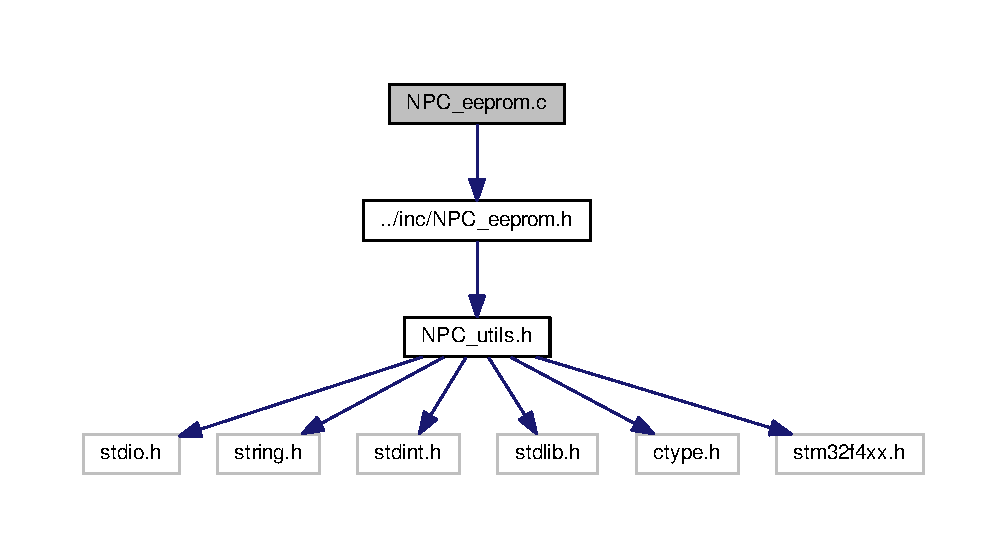
\includegraphics[width=350pt]{d5/d38/_n_p_c__eeprom_8c__incl}
\end{center}
\end{figure}
\subsection*{Functions}
\begin{DoxyCompactItemize}
\item 
void \hyperlink{group___eeprom___init_ga4ec7f9d780da432051aa74ec5892a94c}{eeprom\+\_\+init} (void)
\begin{DoxyCompactList}\small\item\em Initialise communication to the eeprom. \end{DoxyCompactList}\item 
Error\+Status \hyperlink{group___eeprom___trans_ga46c7b6081a89f96d53b6ebc0d0b6f60b}{eeprom\+\_\+write} (uint16\+\_\+t address, uint8\+\_\+t data)
\begin{DoxyCompactList}\small\item\em Write a byte to the eeprom. \end{DoxyCompactList}\item 
uint8\+\_\+t \hyperlink{group___eeprom___trans_gafaa7cca6f6ad1d9ae49522324c825c2f}{eeprom\+\_\+read} (uint16\+\_\+t address)
\begin{DoxyCompactList}\small\item\em Read a byte from the eeprom. \end{DoxyCompactList}\item 
Error\+Status \hyperlink{group___eeprom___trans_ga8c4d6169df1fdb9baeca667b5e9b0058}{eeprom\+\_\+write32\+Bytes} (uint16\+\_\+t base\+Address, uint8\+\_\+t $\ast$data)
\begin{DoxyCompactList}\small\item\em Write a page to the eeprom. \end{DoxyCompactList}\item 
void \hyperlink{group___eeprom___trans_ga7964a5a66da1c4a59a42309a93752217}{eeprom\+\_\+clear} (void)
\begin{DoxyCompactList}\small\item\em Clear eeprom data. \end{DoxyCompactList}\item 
Error\+Status \hyperlink{group___eeprom___trans_ga9dea9d824339ffc184a047749533b96d}{eeprom\+\_\+write\+N\+Bytes} (uint16\+\_\+t base\+Address, uint8\+\_\+t $\ast$data, uint16\+\_\+t N)
\begin{DoxyCompactList}\small\item\em Write N bytes to the eeprom. \end{DoxyCompactList}\item 
Error\+Status \hyperlink{group___eeprom___trans_ga7d9db4a4822fa0c3e5b811615aaed569}{eeprom\+\_\+write4\+Bytes} (uint16\+\_\+t base\+Address, uint8\+\_\+t $\ast$data)
\begin{DoxyCompactList}\small\item\em Write 4 bytes to the eeprom. \end{DoxyCompactList}\item 
uint32\+\_\+t \hyperlink{group___eeprom___trans_ga9a323370ddd02d91c6118f104c015b43}{eeprom\+\_\+read4\+Bytes} (uint16\+\_\+t base\+Address)
\begin{DoxyCompactList}\small\item\em Read a 32byte from eeprom. \end{DoxyCompactList}\item 
void \hyperlink{group___eeprom___trans_gab7c6abb0e0c39a8c152307fb822ffa0c}{eeprom\+\_\+read\+N\+Bytes} (uint16\+\_\+t base\+Address, uint8\+\_\+t $\ast$data, uint16\+\_\+t N)
\end{DoxyCompactItemize}


\subsection{Detailed Description}
This file provides firmware functions to manage data transmission to the eeprom. 

\begin{DoxyAuthor}{Author}
Othniel Konan (Kojey) 
\end{DoxyAuthor}
\begin{DoxyVersion}{Version}
V1.\+1.\+0 
\end{DoxyVersion}
\begin{DoxyDate}{Date}
12-\/\+March-\/2017 
\end{DoxyDate}
\begin{DoxyAttention}{Attention}

\end{DoxyAttention}
\subsubsection*{\begin{center}\copyright{} C\+O\+P\+Y\+R\+I\+G\+HT \end{center} }
\hypertarget{_n_p_c__neopixel_8c}{}\section{C\+:/\+Users/\+Kojey/\+Desktop/\+N\+P\+C/\+Neo\+Pixel\+Clock\+\_\+\+Software/\+Code/\+Libraries/\+N\+P\+C/src/\+N\+P\+C\+\_\+neopixel.c File Reference}
\label{_n_p_c__neopixel_8c}\index{C\+:/\+Users/\+Kojey/\+Desktop/\+N\+P\+C/\+Neo\+Pixel\+Clock\+\_\+\+Software/\+Code/\+Libraries/\+N\+P\+C/src/\+N\+P\+C\+\_\+neopixel.\+c@{C\+:/\+Users/\+Kojey/\+Desktop/\+N\+P\+C/\+Neo\+Pixel\+Clock\+\_\+\+Software/\+Code/\+Libraries/\+N\+P\+C/src/\+N\+P\+C\+\_\+neopixel.\+c}}


This file provides firmware functions to manage the neopixels.  


{\ttfamily \#include \char`\"{}../inc/\+N\+P\+C\+\_\+neopixel.\+h\char`\"{}}\newline
\subsection*{Functions}
\begin{DoxyCompactItemize}
\item 
void \hyperlink{group___neo_pixel___init_gaac78468985e44a3e4d353ea9276b33bc}{neopixel\+\_\+init} (void)
\begin{DoxyCompactList}\small\item\em Initialise the neopixel. \end{DoxyCompactList}\item 
void \hyperlink{group___neo_pixel___state_ga38ad4725462bdc5e86c4ead4f04b9fc2}{T\+I\+M2\+\_\+\+I\+R\+Q\+Handler} (void)
\begin{DoxyCompactList}\small\item\em Timer Handler for neopixel. \end{DoxyCompactList}\item 
void \hyperlink{group___neo_pixel___state_ga8e3cfef785ce221672f825f8785c25b8}{neopixel\+\_\+clear} (void)
\begin{DoxyCompactList}\small\item\em Stop pushing data to the neopixels. \end{DoxyCompactList}\item 
void \hyperlink{group___neo_pixel___state_ga79e34feddcfb2c45ae218166c84bdff4}{neopixel\+\_\+data\+Init} (void)
\begin{DoxyCompactList}\small\item\em Initialise the L\+E\+Dbuffer. \end{DoxyCompactList}\item 
void \hyperlink{group___neo_pixel___state_ga63c196a71ffb007411929e41ba5df41d}{neopixel\+\_\+set\+Pixel\+Colour\+R\+GB} (uint8\+\_\+t n, uint8\+\_\+t r, uint8\+\_\+t g, uint8\+\_\+t b)
\begin{DoxyCompactList}\small\item\em Set the colour of one led. \end{DoxyCompactList}\item 
void \hyperlink{group___neo_pixel___state_gae027558106eef5c81996294f4561fecb}{neopixel\+\_\+set\+Brightness} (uint8\+\_\+t b)
\begin{DoxyCompactList}\small\item\em Set the brightness of the led. \end{DoxyCompactList}\item 
uint32\+\_\+t \hyperlink{group___neo_pixel___colour_ga1d500fbcbecad76feef8835437687ca0}{neopixel\+\_\+colour\+R\+GB} (uint8\+\_\+t r, uint8\+\_\+t g, uint8\+\_\+t b)
\begin{DoxyCompactList}\small\item\em convert R\+GB 3 8bit colour to a 32bit colour \end{DoxyCompactList}\item 
uint32\+\_\+t \hyperlink{group___neo_pixel___colour_ga527ba03b45a249e5e1ea1da4b971b3ac}{neopixel\+\_\+colour\+R\+G\+BW} (uint8\+\_\+t r, uint8\+\_\+t g, uint8\+\_\+t b, uint8\+\_\+t w)
\begin{DoxyCompactList}\small\item\em convert R\+GB 3 8bit colour to a 32bit colour \end{DoxyCompactList}\item 
void \hyperlink{group___neo_pixel___display_ga58d5ceb79029ca8dc5dd8b27b65e4f09}{neopixel\+\_\+set\+Pixel\+Colour\+R\+G\+BW} (uint8\+\_\+t n, uint8\+\_\+t r, uint8\+\_\+t g, uint8\+\_\+t b, uint8\+\_\+t w)
\begin{DoxyCompactList}\small\item\em Set the colour of one led. \end{DoxyCompactList}\item 
void \hyperlink{group___neo_pixel___display_gaecbdecac1da356c5fba07058983d9066}{neopixel\+\_\+set\+Pixel\+Colour} (uint8\+\_\+t n, uint32\+\_\+t c)
\begin{DoxyCompactList}\small\item\em Set the colour of one led. \end{DoxyCompactList}\item 
void \hyperlink{group___neo_pixel___display_ga4daf6edfe83394f425ec51f64d92c49c}{neopixel\+\_\+set\+Pixel\+ColourW} (uint8\+\_\+t n, uint32\+\_\+t c)
\begin{DoxyCompactList}\small\item\em Set the colour of one led. \end{DoxyCompactList}\item 
void \hyperlink{group___neo_pixel___display_ga7a6c2dc149e86a788aede1d6aa5262d7}{neopixel\+\_\+set\+All\+Pixel\+R\+GB} (uint8\+\_\+t r, uint8\+\_\+t g, uint8\+\_\+t b)
\begin{DoxyCompactList}\small\item\em set all the pixel on the line to a specific colour \end{DoxyCompactList}\item 
void \hyperlink{group___neo_pixel___display_ga1ba017c1f338ef2c8e4a48acae35d87e}{neopixel\+\_\+set\+All\+Pixel\+R\+G\+BW} (uint8\+\_\+t r, uint8\+\_\+t g, uint8\+\_\+t b, uint8\+\_\+t w)
\begin{DoxyCompactList}\small\item\em set all the pixel on the line to a specific colour \end{DoxyCompactList}\end{DoxyCompactItemize}


\subsection{Detailed Description}
This file provides firmware functions to manage the neopixels. 

\begin{DoxyAuthor}{Author}
Othniel Konan (Kojey) 
\end{DoxyAuthor}
\begin{DoxyVersion}{Version}
V1.\+1.\+0 
\end{DoxyVersion}
\begin{DoxyDate}{Date}
01-\/\+March-\/2017 
\end{DoxyDate}
\begin{DoxyAttention}{Attention}

\end{DoxyAttention}
\subsubsection*{\begin{center}\copyright{} C\+O\+P\+Y\+R\+I\+G\+HT \end{center} }
\hypertarget{_n_p_c__utils_8c}{}\section{C\+:/\+Users/\+Kojey/\+Desktop/\+N\+P\+C/\+Neo\+Pixel\+Clock\+\_\+\+Software/\+Code/\+Libraries/\+N\+P\+C/\+Framework/src/\+N\+P\+C\+\_\+utils.c File Reference}
\label{_n_p_c__utils_8c}\index{C\+:/\+Users/\+Kojey/\+Desktop/\+N\+P\+C/\+Neo\+Pixel\+Clock\+\_\+\+Software/\+Code/\+Libraries/\+N\+P\+C/\+Framework/src/\+N\+P\+C\+\_\+utils.\+c@{C\+:/\+Users/\+Kojey/\+Desktop/\+N\+P\+C/\+Neo\+Pixel\+Clock\+\_\+\+Software/\+Code/\+Libraries/\+N\+P\+C/\+Framework/src/\+N\+P\+C\+\_\+utils.\+c}}


This file provides utility functions to the N\+PC clock.  


{\ttfamily \#include \char`\"{}../inc/\+N\+P\+C\+\_\+utils.\+h\char`\"{}}\newline
Include dependency graph for N\+P\+C\+\_\+utils.\+c\+:
% FIG 0
\subsection*{Functions}
\begin{DoxyCompactItemize}
\item 
uint32\+\_\+t \hyperlink{group___utils_gafa33c555a40e71b0cc32aa3731f6fabe}{max} (uint32\+\_\+t a, uint32\+\_\+t b, uint32\+\_\+t c)
\begin{DoxyCompactList}\small\item\em Find max between a, b, and c. \end{DoxyCompactList}\item 
void \hyperlink{group___utils_gaf1a8629740f19d111a55636a19c2bf08}{delay} (uint32\+\_\+t microseconds)
\begin{DoxyCompactList}\small\item\em delay for the number of microsecond \end{DoxyCompactList}\end{DoxyCompactItemize}
\subsection*{Variables}
\begin{DoxyCompactItemize}
\item 
uint8\+\_\+t {\bfseries pixel\+\_\+color}
\end{DoxyCompactItemize}


\subsection{Detailed Description}
This file provides utility functions to the N\+PC clock. 

\begin{DoxyAuthor}{Author}
Othniel Konan (Kojey) 
\end{DoxyAuthor}
\begin{DoxyVersion}{Version}
V1.\+1.\+0 
\end{DoxyVersion}
\begin{DoxyDate}{Date}
23-\/\+February-\/2017 
\end{DoxyDate}
\begin{DoxyAttention}{Attention}

\end{DoxyAttention}
\subsubsection*{\begin{center}\copyright{} C\+O\+P\+Y\+R\+I\+G\+HT \end{center} }
%--- End generated contents ---

% Index
\backmatter
\newpage
\phantomsection
\clearemptydoublepage
\addcontentsline{toc}{chapter}{Index}
\printindex

\end{document}
